 %%
%% Beginning of file 'sample62.tex'
%%
%% Modified 2018 January
%%
%% This is a sample manuscript marked up using the
%% AASTeX v6.2 LaTeX 2e macros.
%%
%% AASTeX is now based on Alexey Vikhlinin's emulateapj.cls 
%% (Copyright 2000-2015).  See the classfile for details.

%% AASTeX requires revtex4-1.cls (http://publish.aps.org/revtex4/) and
%% other external packages (latexsym, graphicx, amssymb, longtable, and epsf).
%% All of these external packages should already be present in the modern TeX 
%% distributions.  If not they can also be obtained at www.ctan.org.

%% The first piece of markup in an AASTeX v6.x document is the \documentclass
%% command. LaTeX will ignore any data that comes before this command. The 
%% documentclass can take an optional argument to modify the output style.
%% The command below calls the preprint style  which will produce a tightly 
%% typeset, one-column, single-spaced document.  It is the default and thus
%% does not need to be explicitly stated.
%%
%%
%% using aastex version 6.2
\documentclass{aastex62}

%% The default is a single spaced, 10 point font, single spaced article.
%% There are 5 other style options available via an optional argument. They
%% can be envoked like this:
%%
%% \documentclass[argument]{aastex62}
%% 
%% where the layout options are:
%%
%%  twocolumn   : two text columns, 10 point font, single spaced article.
%%                This is the most compact and represent the final published
%%                derived PDF copy of the accepted manuscript from the publisher
%%  manuscript  : one text column, 12 point font, double spaced article.
%%  preprint    : one text column, 12 point font, single spaced article.  
%%  preprint2   : two text columns, 12 point font, single spaced article.
%%  modern      : a stylish, single text column, 12 point font, article with
%% 		  wider left and right margins. This uses the Daniel
%% 		  Foreman-Mackey and David Hogg design.
%%  RNAAS       : Preferred style for Research Notes which are by design 
%%                lacking an abstract and brief. DO NOT use \begin{abstract}
%%                and \end{abstract} with this style.
%%
%% Note that you can submit to the AAS Journals in any of these 6 styles.
%%
%% There are other optional arguments one can envoke to allow other stylistic
%% actions. The available options are:
%%
%%  astrosymb    : Loads Astrosymb font and define \astrocommands. 
%%  tighten      : Makes baselineskip slightly smaller, only works with 
%%                 the twocolumn substyle.
%%  times        : uses times font instead of the default
%%  linenumbers  : turn on lineno package.
%%  trackchanges : required to see the revision mark up and print its output
%%  longauthor   : Do not use the more compressed footnote style (default) for 
%%                 the author/collaboration/affiliations. Instead print all
%%                 affiliation information after each name. Creates a much
%%                 long author list but may be desirable for short author papers
%%
%% these can be used in any combination, e.g.
%%
%% \documentclass[twocolumn,linenumbers,trackchanges]{aastex62}
%%
%% AASTeX v6.* now includes \hyperref support. While we have built in specific
%% defaults into the classfile you can manually override them with the
%% \hypersetup command. For example,
%%
%%\hypersetup{linkcolor=red,citecolor=green,filecolor=cyan,urlcolor=magenta}
%%
%% will change the color of the internal links to red, the links to the
%% bibliography to green, the file links to cyan, and the external links to
%% magenta. Additional information on \hyperref options can be found here:
%% https://www.tug.org/applications/hyperref/manual.html#x1-40003
%%
%% If you want to create your own macros, you can do so
%% using \newcommand. Your macros should appear before
%% the \begin{document} command.
%%

\usepackage{graphicx}
\usepackage{float}
\usepackage[caption=false]{subfig}
\usepackage{enumitem}

%\usepackage{natbib}
%\usepackage{pdflscape}

%% AASTeX v6.* now includes \hyperref support. While we have built in specific
%% defaults into the classfile you can manually override them with the
%% \hypersetup command. For example,
%%
%%\hypersetup{linkcolor=red,citecolor=green,filecolor=cyan,urlcolor=magenta}
%%
%% will change the color of the internal links to red, the links to the
%% bibliography to green, the file links to cyan, and the external links to
%% magenta. Additional information on \hyperref options can be found here:
%% https://www.tug.org/applications/hyperref/manual.html#x1-40003

%% If you want to create your own macros, you can do so
%% using \newcommand. Your macros should appear before
%% the \begin{document} command.
%%
\newcommand{\vdag}{(v)^\dagger}
\newcommand\aastex{AAS\TeX}
\newcommand\latex{La\TeX}
\newcommand{\exampleConstant}{0.04}
\newcommand{\degree}{^\circ}
\newcommand{\spitzer}{{\it Spitzer}}
\newcommand{\kepler}{{\it Kepler}}

%% Reintroduced the \received and \accepted commands from AASTeX v5.2
%\received{July 1, 2016}
%\revised{September 27, 2016}
%\accepted{\today}
%% Command to document which AAS Journal the manuscript was submitted to.
%% Adds "Submitted to " the arguement.
%\submitjournal{ApJ}

%% Mark up commands to limit the number of authors on the front page.
%% Note that in AASTeX v6.1 a \collaboration call (see below) counts as
%% an author in this case.
%
%\AuthorCollaborationLimit=3
%
%% Will only show Schwarz, Muench and "the AAS Journals Data Scientist 
%% collaboration" on the front page of this example manuscript.
%%
%% Note that all of the author will be shown in the published article.
%% This feature is meant to be used prior to acceptance to make the
%% front end of a long author article more manageable. Please do not use
%% this functionality for manuscripts with less than 20 authors. Conversely,
%% please do use this when the number of authors exceeds 40.
%%
%% Use \allauthors at the manuscript end to show the full author list.
%% This command should only be used with \AuthorCollaborationLimit is used.

%% The following command can be used to set the latex table counters.  It
%% is needed in this document because it uses a mix of latex tabular and
%% AASTeX deluxetables.  In general it should not be needed.
%\setcounter{table}{1}

%%%%%%%%%%%%%%%%%%%%%%%%%%%%%%%%%%%%%%%%%%%%%%%%%%%%%%%%%%%%%%%%%%%%%%%%%%%%%%%%
%%
%% The following section outlines numerous optional output that
%% can be displayed in the front matter or as running meta-data.
%%
%% If you wish, you may supply running head information, although
%% this information may be modified by the editorial offices.
\shorttitle{NIRCam Lab Stability Studies}
\shortauthors{Schlawin et al.}
%%
%% You can add a light gray and diagonal water-mark to the first page 
%% with this command:
% \watermark{text}
%% where "text", e.g. DRAFT, is the text to appear.  If the text is 
%% long you can control the water-mark size with:
%  \setwatermarkfontsize{dimension}
%% where dimension is any recognized LaTeX dimension, e.g. pt, in, etc.
%%
%%%%%%%%%%%%%%%%%%%%%%%%%%%%%%%%%%%%%%%%%%%%%%%%%%%%%%%%%%%%%%%%%%%%%%%%%%%%%%%%

%% This is the end of the preamble.  Indicate the beginning of the
%% manuscript itself with \begin{document}.

\begin{document}

\title{Lessons Learned about JWST Transiting Planet Time Series from Ground-based Studies of the NIRCam Detectors}

%% LaTeX will automatically break titles if they run longer than
%% one line. However, you may use \\ to force a line break if
%% you desire. In v6.1 you can include a footnote in the title.

%% A significant change from earlier AASTEX versions is in the structure for 
%% calling author and affilations. The change was necessary to implement 
%% autoindexing of affilations which prior was a manual process that could 
%% easily be tedious in large author manuscripts.
%%
%% The \author command is the same as before except it now takes an optional
%% arguement which is the 16 digit ORCID. The syntax is:
%% \author[xxxx-xxxx-xxxx-xxxx]{Author Name}
%%
%% This will hyperlink the author name to the author's ORCID page. Note that
%% during compilation, LaTeX will do some limited checking of the format of
%% the ID to make sure it is valid.
%%
%% Use \affiliation for affiliation information. The old \affil is now aliased
%% to \affiliation. AASTeX v6.1 will automatically index these in the header.
%% When a duplicate is found its index will be the same as its previous entry.
%%
%% Note that \altaffilmark and \altaffiltext have been removed and thus 
%% can not be used to document secondary affiliations. If they are used latex
%% will issue a specific error message and quit. Please use multiple 
%% \affiliation calls for to document more than one affiliation.
%%
%% The new \altaffiliation can be used to indicate some secondary information
%% such as fellowships. This command produces a non-numeric footnote that is
%% set away from the numeric \affiliation footnotes.  NOTE that if an
%% \altaffiliation command is used it must come BEFORE the \affiliation call,
%% right after the \author command, in order to place the footnotes in
%% the proper location.
%%
%% Use \email to set provide email addresses. Each \email will appear on its
%% own line so you can put multiple email address in one \email call. A new
%% \correspondingauthor command is available in V6.1 to identify the
%% corresponding author of the manuscript. It is the author's responsibility
%% to make sure this name is also in the author list.
%%
%% While authors can be grouped inside the same \author and \affiliation
%% commands it is better to have a single author for each. This allows for
%% one to exploit all the new benefits and should make book-keeping easier.
%%
%% If done correctly the peer review system will be able to
%% automatically put the author and affiliation information from the manuscript
%% and save the corresponding author the trouble of entering it by hand.

\correspondingauthor{Everett Schlawin}
\email{eas342 AT EMAIL Dot Arizona .edu}

\author[0000-0001-8291-6490]{Everett Schlawin}
\affiliation{Steward Observatory \\
933 North Cherry Avenue \\
Tucson, AZ 85721, USA}

\author{Rafia Bushra}
\affiliation{Steward Observatory \\
933 North Cherry Avenue \\
Tucson, AZ 85721, USA}

\author{Stephanie Striegel}
\affiliation{Department of Physics \& Astronomy \\
San Jose State University \\
One Washington Square \\
San Jose, CA 95192, USA}
\affiliation{NASA Ames Research Center \\
Space Science and Astrobiology Division \\
Moffett Field, CA 94035, USA}

\author{Xander Levinson}
\affiliation{Department of Astronomy \& Astrophysics \\
University of California, Santa Cruz \\
1156 Highland Street \\
Santa Cruz, CA 95062, USA}
\affiliation{NASA Ames Research Center \\
Space Science and Astrobiology Division \\
Moffett Field, CA 94035, USA}


\author{Karl Misselt}
\affiliation{Steward Observatory \\
933 North Cherry Avenue \\
Tucson, AZ 85721, USA}

\author{Jarron Leisenring}
\affiliation{Steward Observatory \\
933 North Cherry Avenue \\
Tucson, AZ 85721, USA}

\author{Kenneth Don}
\affiliation{Steward Observatory \\
933 North Cherry Avenue \\
Tucson, AZ 85721, USA}

\author{Douglas Kelly}
\affiliation{Steward Observatory \\
933 North Cherry Avenue \\
Tucson, AZ 85721, USA}

\author{Thomas Beatty}
\affiliation{Steward Observatory \\
933 North Cherry Avenue \\
Tucson, AZ 85721, USA}



\author{Thomas P Greene}
\affiliation{NASA Ames Research Center \\
Space Science and Astrobiology Division \\
Moffett Field, CA 94035, USA}

\author{Marcia Rieke}
\affiliation{Steward Observatory \\
933 North Cherry Avenue \\
Tucson, AZ 85721, USA}


%% Note that the \and command from previous versions of AASTeX is now
%% depreciated in this version as it is no longer necessary. AASTeX 
%% automatically takes care of all commas and "and"s between authors names.

%% AASTeX 6.1 has the new \collaboration and \nocollaboration commands to
%% provide the collaboration status of a group of authors. These commands 
%% can be used either before or after the list of corresponding authors. The
%% argument for \collaboration is the collaboration identifier. Authors are
%% encouraged to surround collaboration identifiers with ()s. The 
%% \nocollaboration command takes no argument and exists to indicate that
%% the nearby authors are not part of surrounding collaborations.

%% Mark off the abstract in the ``abstract'' environment. 
\begin{abstract}

JWST transmission and emission spectra of transiting exoplanets will provide invaluable glimpses at exoplanet atmospheres.
These spectra will reveal the composition and temperature structure at a level never achieved before.
This promising science from JWST, however, will require exquisite precision and understanding of systematic errors that can impact the time series of planets crossing in front of and behind their host stars.
This is especially true if JWST is used to search for biosignatures in temperature atmospheres on Earth-sized planets that may contain liquid water.
Here, we provide the lessons learned from ground-based characterization of the NIRCam H2RG detectors, which will be used for exoplanet spectra.
%and are the same type of detectors used in JWST's NIRISS and NIRSpec instruments.
We summarize the lessons learned from tests at NASA Goddard, NASA Johnson and the University of Arizona detector lab.

\end{abstract}

%% Keywords should appear after the \end{abstract} command. 
%% See the online documentation for the full list of available subject
%% keywords and the rules for their use.
\keywords{stars: atmospheres --- stars: individual (\objectname{KIC 12557548}) ---
stars: variables: general}

%% From the front matter, we move on to the body of the paper.
%% Sections are demarcated by \section and \subsection, respectively.
%% Observe the use of the LaTeX \label
%% command after the \subsection to give a symbolic KEY to the
%% subsection for cross-referencing in a \ref command.
%% You can use LaTeX's \ref and \label commands to keep track of
%% cross-references to sections, equations, tables, and figures.
%% That way, if you change the order of any elements, LaTeX will
%% automatically renumber them.

%% We recommend that authors also use the natbib \citep
%% and \citet commands to identify citations.  The citations are
%% tied to the reference list via symbolic KEYs. The KEY corresponds
%% to the KEY in the \bibitem in the reference list below. 

\section{Introduction} \label{sec:intro}

JWST will provide powerful new measurements of exoplanet atmospheres with spectroscopy from 0.6 to 12 $\mu$m
\citep{beichman2014pasp,greene2016jwst_trans,howe2017informationJWST,barstow2015jwstSystematics,schlawin2018JWSTforecasts}.
The sensitivity of JWST combined with its unprecedented wavelength coverage on exoplanets will enable it to measure the abundance of carbon-bearing molecules (CO, CO$2$ and CH$_4$) as well as study cooler, smaller planets than previously characterized.

JWST has also been considered for observations of potentially habitable Earth-like planets that orbit their stars at a distance where water could be in liquid form on their surface.
The TRAPPIST-1 system \citep{gillon2016trappist1Discovery,gillon2017trappist-1sevenp} presents an exciting opportunity to study Earth-sized stars orbiting a 0.1~R$_\odot$ M-type star.
By putting together 10 to 30 transits, it will be possible to collect enough photons to detect CO$_2$ \citep{barstow2016trappist1habitable,krissansen-totton2018trappist1eJWST,lustig-yaeger2019detectabilityTRAPPIST-1}.
Optimistically, 30 transits may contain enough photons to detect O$_3$ in the atmosphere of TRAPPIST-1 d with JWST if clouds have a minimal impact on its atmosphere \citep{barstow2016trappist1habitable}.
More detailed modeling of atmospheric evolution indicates that biogenic oxygen may be too difficult to detect with any JWST instrument but desiccated oceans may produce detectable abiogenic oxygen \citep{lustig-yaeger2019detectabilityTRAPPIST-1}.
Alternatively, 10 transits of TRAPPIST-1e could be sufficient if the planet's atmosphere has CO$_2$ and CH$_4$ biosignatures similar to early-Earth \citep{krissansen-totton2018trappist1eJWST}.
A critical question in studying planets like TRAPPIST-1 d/e, however, is whether photon-limited performance is possible with JWST observations.

Experience with the Hubble Space Telescope (HST), \spitzer, and \kepler\ shows that many systematics can affect high precision time series and prevent photon-limited performance unless corrected for \citep[e.g.][]{beichman2014pasp}.
Many of these effects are detector-related including charge trapping on HST's detector \citep{berta2012flat_gj1214,zhou2017chargeTrap}, intra-pixel sensitivity on the short wavelength bands of \spitzer\ IRAC \citep{moralesCalderon2006LdwarfsWeatherIPC} and sensitivity to pointing jitter with \kepler\footnote{https://keplerscience.arc.nasa.gov/K2/Performance.shtml} \citep{beichman2014pasp}.

The NIRCam instrument \citep{rieke2005nircamSPIE} contains a slitless grism mode with its long wavelength channel \citep{greene2017jatisNIRCam}.
This slitless grism mode is analogous to the WFC3 grism on HST that has been successfully employed on many transiting planets \citep[e.g.][]{deming13,kreidberg2014wasp43,sing2016continuum,wakeford2017hatp26}.
The NIRCam grism mode will collect moderate resolution R$\sim$1100-1700 spectra over the wavelength range from 2.4 to 5.0~$\mu$m.
This grism mode can be used simultaneously with short wavelength weak lens imaging or the Dispersed Hartmann Sensor mode \citep{schlawin2017dhs}. If it becomes an approved and implemented mode, the DHS will permit spectroscopy simultaneous from 1.0 to 2.0~$\mu$m because of a dichroic beamsplitter that divides the light from NIRCam into two different channels.
The DHS mode will permit time series spectroscopy on very bright targets ($K_S \sim 1$) inaccessible by other modes.

Given the finite lifetime of the JWST mission set by onboard fuel, it is important to understand the systematic errors before launch to maximize the science return of the observatory.
We discuss the major sources of systematic errors that can affect the NIRCam instrument.
Parallel efforts to characterize other instrument's noise sources are being done, such as with MIRI's detectors \citep{matuso2019siAsDetectorStability}.

Section \ref{sec:knownEffects} lists the known systematic effects that can impeded high precision time series and increase the noise above the photon and read noise.
Section \ref{sec:experiments} describes the experiments on the ground that are used to prepare for JWST observations in flight.


\section{Known Detector Effects}\label{sec:knownEffects}
An ideal HgCdTe detector simply counts the photons incident on its surface (as described in section \ref{sec:detectorPrimer}).
However, there are many non-ideal effects that can affect the stability of a light curve of a transiting exoplanet.
Here, we review many of the known noise sources that could impact the stability of a time series beyond photon counting statistics. These known detector effects that can impact stability are listed briefly and then in more detail as related to the JWST NIRCam detectors below that.

\begin{itemize}[noitemsep]
	\item \textbf{Pre-amp reset offsets:} (an Asic-related effect) 
The resets cause discontinuities in the pedestal level of all pixels between frames.
Pre-amp resets can also appear in slope images (DN/second) because NIRCam's amplifiers are reset once per frame (not once per integration).
This is an effect where averaging over more pixels does not decrease the noise, but reference pixel or background subtraction can.
These are discussed further in Section \ref{sec:preAmp}.
	\item \textbf{Amplifier Boundary Discontinuities} The NIRCam detectors can be read out in full frame, stripe and window modes. The full frame and stripe modes make use of 4 amplifiers that can record or reset the accumulated electrons in 4 pixels simultaneously in parallel. The parallel operation of the amplifiers reduces the frame time and reset time by a factor of 4 but can introduce subtle voltage biases between regions of the detector. If these voltage biases are not corrected, they can potentially introduce discontinuities in a spectrum, which crosses amplifier boundaries.
	\item \textbf{1/f noise:} The JWST HgCdTe readout electronics have a p-type metal-oxide semiconductor field-effect transistor (PFET) source follower that introduces noise to the images as well as DC biases in the ASIC electronics \citep{rauscher2011irsSquared}.
	This is a noise source where most of the noise power is concentrated at low frequencies.
	1/f noise causes spatial correlations in the fast-read direction (along detector rows). It is highly correlated between amplifiers, suggesting that it is caused by a common reference voltage. 1/f noise can be reduced by subtracting the values from background pixels or reference pixels.
	\item \textbf{Intrapixel sensitivity:} Telescope pointing drifts and jitter can impact the amount of flux measured if the response of pixels is not perfectly uniform.
	This has a particularly strong impact on the time series from the Spitzer IRAC instrument \citep{ingalls2016spitzerRepeatability}.
	It can also appear on JWST detectors because the sub-pixel flat field is not uniform.
	Crosshatching patterns on HgCdTe detectors (which all JWST near-infrared instruments use) exist at the sub-pixel level  \citep{shapiro2018crosshatch,ninan2019crosshatchHPF}
	\item \textbf{Even/odd offsets:} Alternating columns have different bias levels. Additionally, there are offsets between columns that can change from frame to frame, especially on NIRCam's LW detector.
	These can be reduced with reference pixels or background subtraction.
	\item \textbf{kTC noise:} Each reset at the beginning of an integration introduces thermal noise associated with the unknown amount of charge stored in a pixel at the reset voltage level.
	Fortunately, the bias offset produces by kTC noise will easily subtract out when fitting a slope image from the multiple samples up the ramp.
	This noise would  only become relevant when attempting to make use of the first group of a ramp (such as when only 1 group is commanded).
	\item \textbf{Detector Temperature Fluctuations:} The JWST detectors are sensitive to temperature changes on the focal plane arrays. For example, laboratory tests show that 100 mK temperature fluctuations can result in $\sim$ 80 ADU changes on the detector that are not corrected by reference pixels \citep{hall2005jwstArrays}. Fortunately, the detectors are actively thermally controlled to keep the temperature fluctuations to mostly $\lesssim$ 1 mK.
The one exception is that the Long Wavelength A-side detector (A5) exhibited $\sim$ 20 min oscillations with an amplitude of 15-20 mK when using the Temperature Monitor Control (TMC) 1 active thermal control.
Fortunately, the TMC 2 control does not undergo these oscillations and will be employed in orbit.
If necessary, the effect of temperature fluctuations can be calibrated to $\pm 1 e^-$ for excursions less than $\pm$ 50 mK \citep{hall2005jwstArrays}.
	\item \textbf{ASIC Temperature Fluctuations:} The asic temperature will change as the operating mode. For example, in the CV3 stability test, the temperature of the A asic changed by $\sim$80 mK when the readout mode was switched from full frame to subarray.
	This temperature change is expected to be smaller in flight due to adjustments in the operations to run all four amplifiers regardless of how many are used to collect science data.
	\item \textbf{Elevated Columns} There is correlated noise along a column in many frames. These elevated columns can sometimes even move with time.
	\item \textbf{Random Telegraph Noise (RTN)} Some of the pixels will exhibit spontaneous changes jumps in signal even with no illumination. Fortunately, RTN appears in only $\sim$1000 pixels out of 4$\times 10^6$ on the array.
	\item \textbf{Detector Fringing} \textbf{\textcolor{red}{Add more details and citations}} The thin $\sim 5\mu$m layers of the H2RG detectors will cause interference patterns on the array due to constructive and destructive interference of light at wavelengths similar to the thickness of the layers. If the detector fringe pattern changes with time, it will change the throughput of a grism image.
	\item \textbf{Charge Trapping} A major correlated error source on HST WFC3 is the ``hook effect'' \citep{berta2012flat_gj1214}.
	The hook effects is due to charge can be trapped within the detector's depletion region (initially lowering the flux) and then released at later times (increasing the flux) \citep{zhou2017chargeTrap}.
	JWST's NIRCam instrument has very lower rates of persistence ($<$1 DN/sec) at 100 seconds after saturation, so it is expected that charge trapping will be a minor concern for JWST's HgCdTe detectors.
\end{itemize}

It should be noted that the detector effects related to the asic circuit can be specific to the ``personality'' of each asic. The asics all have different asic load files which are tuned to minimize the power consumption and dark current in a particular asic. Since the asic load files are specific to each detector, they may exhibit different noise properties.
Some caution should be taken when comparing noise tests with engineering grade or rejected detectors with the flight detectors.

\subsection{Pre-amp Reset Offsets from the Lockheed CV Test}\label{sec:preAmp}

The NIRCam detectors' pre-amplifiers (pre-amps) have a reference voltage that can drift with time.
This can affect the pedestal level of all pixels over long ($\gtrsim$ 20 minute timescales).
These pre-amplifier levels can either be reset at the beginning of an integration with samples up the ramp or with each frame up the ramp.
The NIRCam detectors are reset once per frame to prevent large amplifier drifts over an integration \citep{robberto2014refPixPreAmp}.
One set of darks was collected at Lockheed CV with a reset only once per integration to study the effects of the pre-amplifier resets.

In the Lockheed CV test, the pedestal level of all pixels could be seen to drift over 19.3 minute dark integrations by 5 to 100 DN.
The drift was usually linear over these 19 minute exposures, but in one case was observed to drift downward from 100 DN to -50 DN and back to 100 DN \citep{robberto2014refPixPreAmp}.
The timescales for pre-amp resets are relevant to exoplanet time series, which have transit durations of $\sim$0.5 to 3 hours for typical targets.
However, reference pixel subtraction can efficiently remove pre-amp drifts, so with proper data reduction and subarrays that include reference pixels, the pre-amp drifts can be dramatically reduced.
It is also likely that background subtraction can mitigate the pre-amp reset offsets from time series integrations.
The NIRCam grism subarrays and dispersed source location are placed at the edge of the NIRCam Long Wavelength detector to ensure reference pixels are saved with active pixels.

Figure \ref{fig:ampResetDark} shows an example time series of the reference pixels for a dark exposure.
The pedestal/bias level of the reference pixels undergoes a sharp jump between each frame (10.7 seconds in duration).
These pre-amp resets per frame causes discontinuities over every frame within an integration, but there is an upside:
Over long timescales (10$^3$ seconds), these resets pre-amp resets will keep the bias drifts hovering around zero without any long slopes or drifts.
This is helpful in keeping the detector counts below the 65,536 DN saturation limit and thus pre-amp resets permit a larger usable well depth over the counts from 0 to 65,536 DN.
Without pre-amp resets, the counts in a detector could potentially drift towards 65,536 DN and shrinks the usable well depth.

\begin{figure}[!hbtp]
\centering
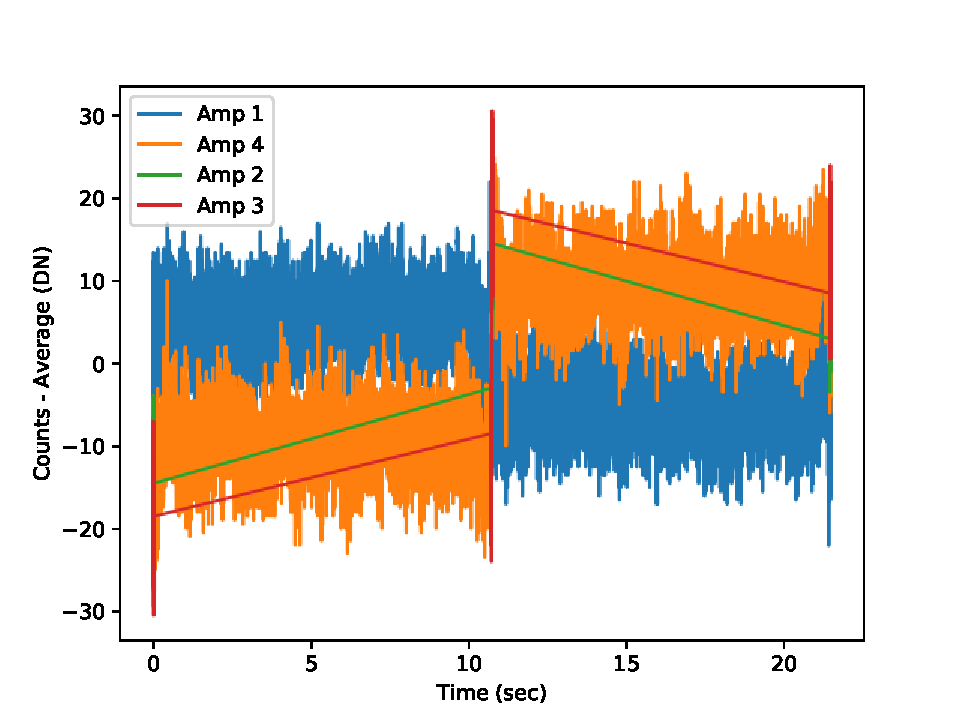
\includegraphics[width=.49\columnwidth]{allamps.pdf}
\includegraphics[width=.49\columnwidth]{allamps_long_dark.pdf}
\caption{Reference pixel time series for a two frame integration (Left) and a long dark integration of 108 frames (Right). Each of the plots show that the pre-amplifier resets between frames in an integration cause discontinuities in the reference signal. Amplifiers 1 and 4 track the time all through a frame with the side reference pixels, whereas amplifiers 2 and 3 in the middle only contain information on the bottom and top reference pixels at the beginning and ending of a frame.
The long dark exposure example of 108 integrations shows the behavior over long timescales.}\label{fig:ampResetDark}
\end{figure}

\subsection{Amplifier Boundary Discontinuities}

NIRCam's STRIPE mode and full frame mode both employ 4 amplifiers to simultaneously read out or reset 4 pixels at once.
This simultaneous use of 4 amplifiers reduces the frame time by a factor of 4 and thus increases the brightness of objects that can be detected before saturation as well as increase the number of reads up a detector pixel to average down readout noise.
On the flip side, the four amplifiers will have different behaviors such as offsets in the bias level.
The differential biases between the amplifiers will show up as step function changes in the slope of the image at the amplifier boundaries (512, 1024 and 1536), as visible in Figure \ref{fig:ampOffsetsOtisGrismSlope} (top panel).
If a spectrum of a source is extracted without any vertical background extraction, the amplifier offsets cause sharp discontinuities in the summed spectrum.

Fortunately, the amplifier offsets are efficiently removed by reference pixels.
For example, we subtract the median of the 4 reference pixels from each column and this efficiently removes the bias signal from each amplifier shown in Figure \ref{fig:ampOffsetsOtisGrismSlope} (middle panel and bottom panel).
It should be noted, however, that there are gradients in the bias signal within each amplifier. If we simply subtract the median value of all reference pixels within an amplifier without applying them on a per-column basis, there are still discontinuities in the spectrum.
In addition to reference pixels, background subtraction along each column removes the amplifier boundary effect.
If the boundaries somehow proved to be an issue for time series spectra, the WINDOW subarray mode, which uses a single amplifier (at the cost of 4 times the frame time) is an option.

\begin{figure}[!hbtp]
\centering
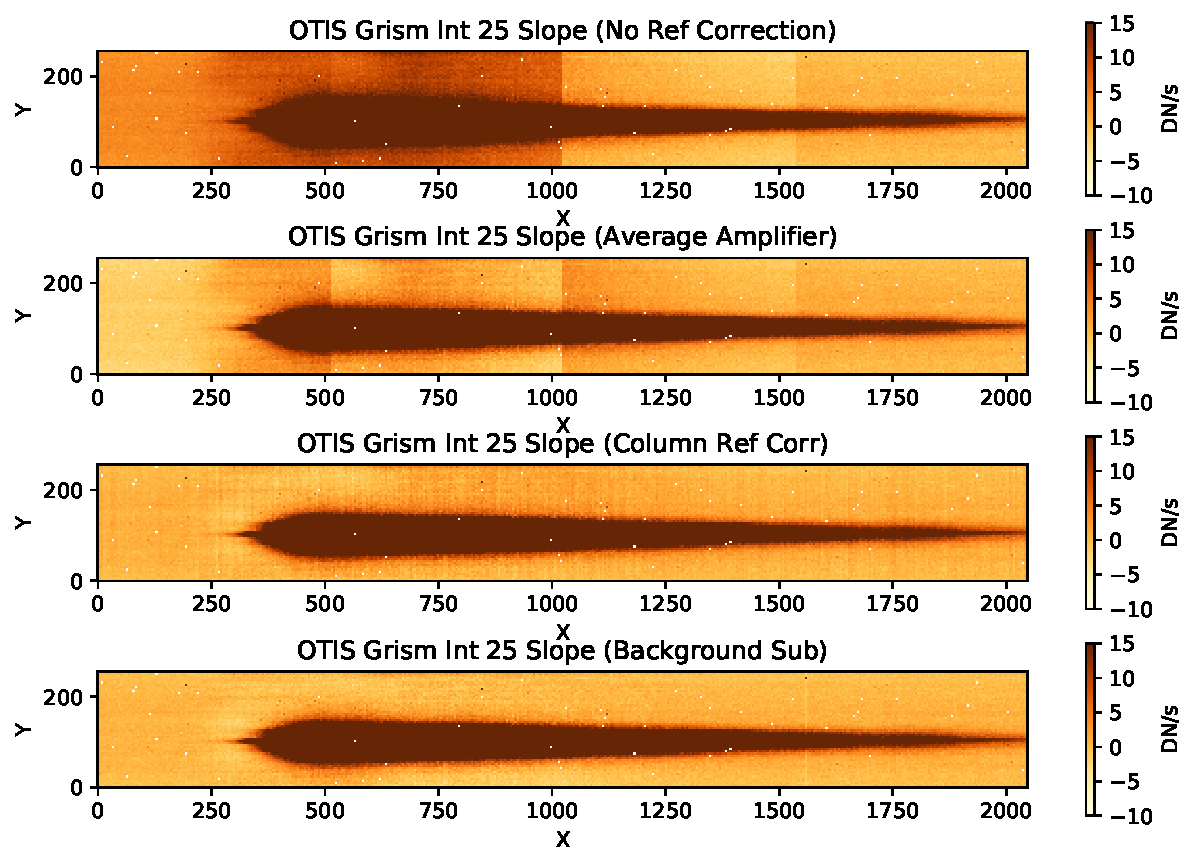
\includegraphics[width=.79\columnwidth]{amplifier_offsets_in_otis_lw_grism.pdf}
\caption{An example slope image from the LW OTIS Stability test.
{\it First Panel:} No reference pixel correction is applied, leaving offsets at the amplifier boundaries.
{\it Second Panel:} Averaging all the reference pixels within an amplifier and subtracting the result reduces the offsets between amplifiers but there are still noticeable boundaries at X= 512, 1024 and 1536.
{\it Third Panel:} Reference pixel correction using the 4 non-illuminated pixels in each column significantly reduces offsets between amplifiers, but introduces read noise to each column.
{\it Fourth Panel:} Background subtraction with the mean value of the pixels below Y=15 and above Y=190 eliminates offsets between amplifiers without introducing any substantial new noise source.
}\label{fig:ampOffsetsOtisGrismSlope}
\end{figure}

\clearpage

\subsection{1/f Noise}
The readout circuitry for NIRCam and other JWST NIR instruments introduces correlated noise from pixel-to-pixel.
This is visible when examining the time series of pixels as they are read out within a frame in the order they are addressed.\footnote{See a diagram of the readout directions at \url{https://jwst-docs.stsci.edu/near-infrared-camera/nircam-instrumentation/nircam-detector-overview/nircam-detector-readout}}
The power spectrum of this pixel-by-pixel time series reveals high power at low frequencies that drops roughly like a 1/f power law in the power spectrum of the time series.
Figure \ref{fig:pixelTSeriesPSpec} shows the average Lomb Scargle periodogram from amplifier over 108 dark frames.
To create the periodogram, the reference pixels are used to remove amplifier offsets between frames.
Next, the average of all frames is subtracted to remove the bias and all pixels that deviate by more than 80 DN from the average are masked to eliminate bad pixels.
The periodogram shows many spikes at high frequency including one at the line reset time of 524 clock cycles, which is the time to read out all the pixels in a row for the amplifier and line overheads before moving to the next row.

The 1/f noise is compared to a simulated time series with the same robust standard deviation but with Gaussian white noise where each pixel is independent and identically distributed as a Gaussian.
It is clear from Figure \ref{fig:pixelTSeriesPSpec} that the 1/f noise and the periodic signatures significantly increase the power over uncorrelated white noise (green line) at low frequencies.
1/f rises above the white noise level at 70 cycles / 1400 Hz for amplifier 1 and the intersection ranges from 70 to 135 across the 4 amplifiers.

\begin{figure*}[!hbtp]
\centering
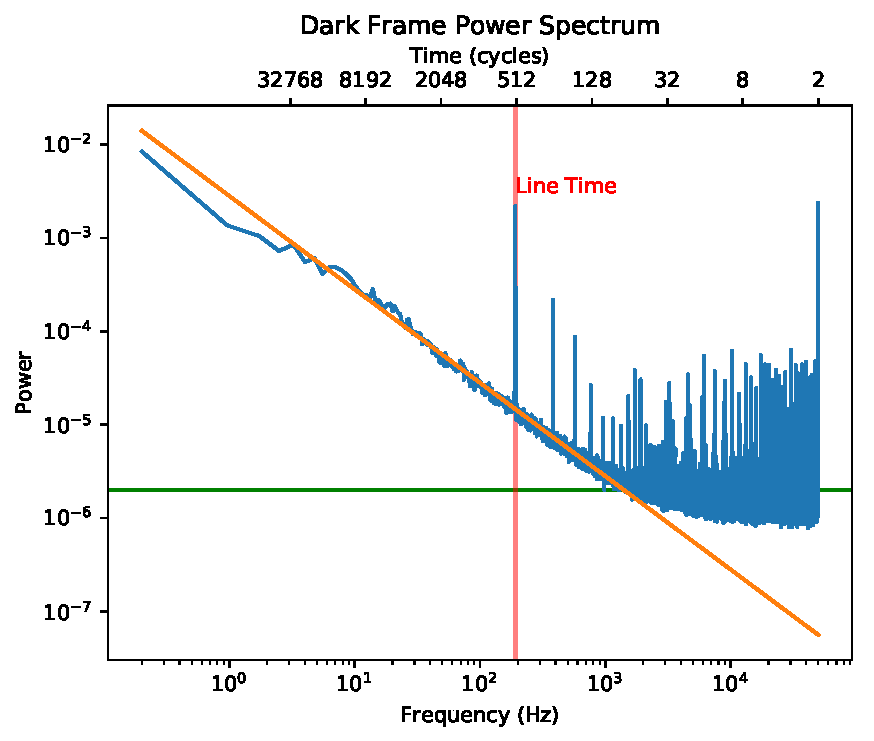
\includegraphics[width=.4\columnwidth]{avg_psd_amp_1.pdf}
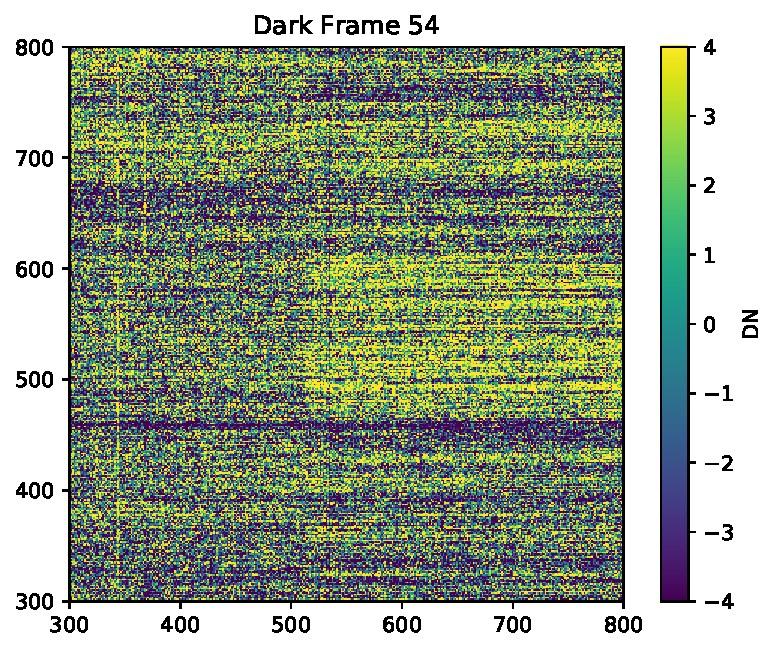
\includegraphics[width=.4\columnwidth]{preamp_removed_grp_54.pdf}
\caption{{\it Left:} The average Lomb Scargle periodogram from Amplifier 1's time series over 108 groups.
The noise in the spectrum is close to a 1/f power law (orange line) from 10 to 1000 Hz.
Above 1000 Hz, it is closer to white noise (green line) with spikes at specific frequencies.
{\it Right:} This 1/f noise introduced in the readout circuit causes prominent correlated noise along the fast-read direction (horizontal) on a dark frame.
The amplifier offsets have been removed, but the 1/f noise from these adjacent amplifiers (separated at X=512) shows different behavior.
}\label{fig:pixelTSeriesPSpec}
\end{figure*}

The 1/f noise can be reduced by subtracting reference pixels and/or active pixels over the aperture of interest.
As the power spectrum shows, the 1/f noise begins to contribute significantly for frequencies below 1000 Hz (ie. timescales longer than 100 cycles as measured in the 10$\mu$s time to address the pixels).
Ideally, source apertures would be less than 100 pixels wide so that background subtraction along rows will remove the 1/f noise but this is impossible for grism spectra dispersed along the rows.
NIRCam has a "GRISMC" grism that will disperse along the column direction but this mode would not work with horizontal stripe subarrays and would therefore saturate on bright targets with $K \lesssim 5.5$.
The benefits of a horizontal stripe subarray and a faster sampling rate must be weighed against the price of correlated 1/f noise along the spectrum that is not easily subtracted.

\subsection{Fringing}

The thin layer of NIRCam's HgCdTe detector can result in an interference pattern much like thin film interference on bubbles.
Fringing will be less noticeable when many wavelengths are mixed together, but with grism spectra where the wavelengths are separated, the interference effects are more pronounced.
We investigate whether this can manifest itself on the spectrum with the NIRCam grism by looking for periodic signatures that vary in frequency as a function of wavelength.

Figure \ref{fig:cv3ExtractedSpectrum} shows an extracted spectrum from Cryogenic Vacuum 3 testing where a broadband point source is dispersed by the grism.
The slope image is calculated from the raw ramp using the internal NIRCam ramps-to-slopes pipeline \texttt{nchdas}.
The background is subtracted with a 2nd order polynomial fit and the flux is extracted with an optimally weighted summation \citep[e.g.][]{horne1986optimalE}.
The spectrum is normalized by a 3rd order spline fit with 400 knots to remove the broad shape of the spectrum and the throughput curves.
The resulting spectrum shows high frequency ($\sim$0.2 px$^{-1}$ to $\sim$0.5 px$^{-1}$) variations far in excess of the photon and read noise.
These oscillations increase in frequency at longer wavelengths (X pixels).
The variations have peak-to-valley amplitudes of about 10\%.
However, we expect that the fringing structure will hold relatively constant during time so long as the pointing is stable at the sub-pixel level.

\begin{figure}[!hbtp]
\centering
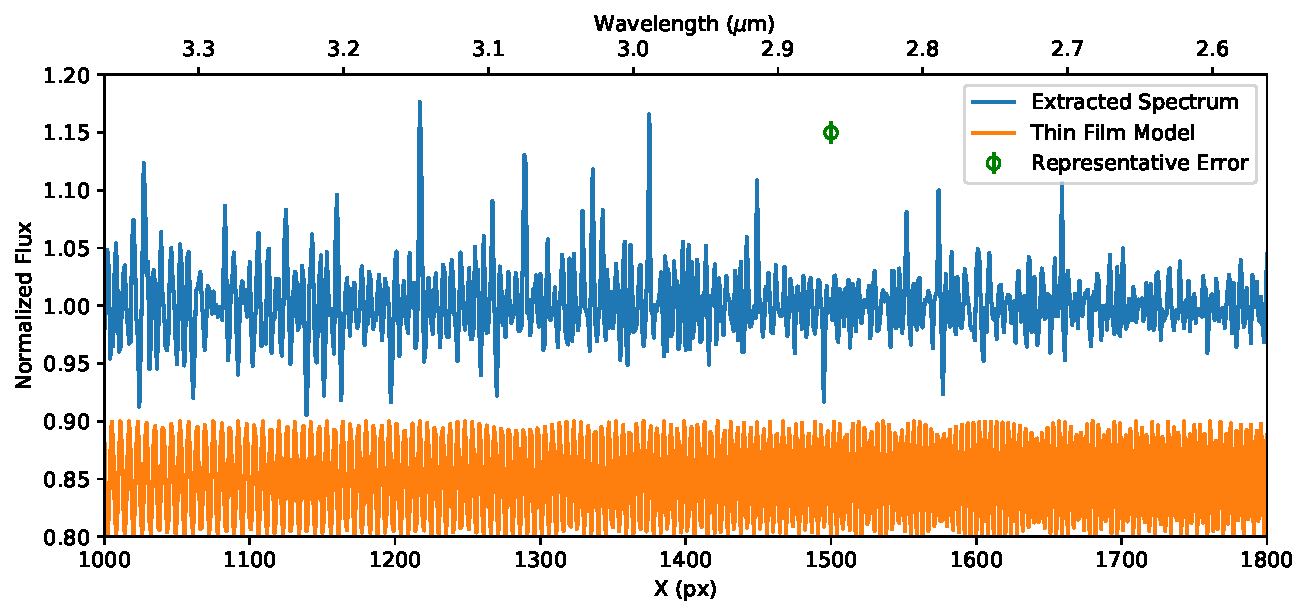
\includegraphics[width=.99\columnwidth]{fringing_grism_cv3.pdf}
\caption{A CV3 grism spectrum over the time series grism test shows evidence for fringing and where the oscillations exceed the photon and read noise (green point).
An illustrative sinusoidal function is plotted for comparison to better see how the frequencies change as a function of wavelength (X pixel).
}\label{fig:CV3GrismSpecFringing}
\end{figure}

\subsection{Subpixel Crosshatching}

\subsubsection{Subpixel Crosshatching Characterization}
The flat field of the ALONG detector, which is used for NIRCam grism series, has a pronounced crosshatch pattern visible in Figure \ref{fig:crossHatchA5}.
The patterns are located at 23.1$\degree$ , 90.9$\degree$, and 158.6 $\degree$ counter-clockwise from the $+$X direction of the detector.
The angle between these lines are 67.8$\degree$, 67.7$\degree$ and 44.5$\degree$.
These angles and patterns can be analyzed with a 2D power spectrum as shown in Figure \ref{fig:crossHatchA5}.

The angles of the crosshatch patterns are determined by the crystal pattern of HgCdTe.
HgCdTe has a zincblende structure with tetrahedral bond angles where each Hg or Cd atom is surrounded by 4 Te atoms \citep{gemain2012mercVacanciesHgCdTe}.
HgCdTe detectors are manufactured using molecular beam epitaxy upon a substrate, a process which can result in topological defects with peak to valley amplitudes of 5-20 nm in height variations \citep{chang2008surfaceMorphologyHgCdTe}.
The surface morphology of the HgCdTe crystal shows that the crosshatch patterns are are oriented along the intersection of the (211) growth plane of the crystal and the 8 HgCdTe slip planes.

The relative angles of the HgCdTe slip planes and (211) growth plane are 44.42$\degree$, 67.79$\degree$ and 67.79$\degree$ \citep{chang2008surfaceMorphologyHgCdTe}, very close to the observed crosshatch angles.
One possible projection of a zincblende structure is shown in Figure \ref{fig:crossHatchA5}.
In this perspective, the projected bond angles are 44.4$\degree$, 67.8$\degree$ and 67.8$\degree$.
These surface topological variations with crosshatch patterns are likely related to the observed patterns in the flat fields, which appear as quantum efficiency variations.
We deduce that the crosshatch pattern is mostly likely related to the crystal lattice structure of the HgCdTe substrate and not the pixel circuitry.

The crosshatch structure of the detectors extends down to the subpixel level, so it will not be fully corrected with a flat field division.
This sub-pixel structure has been imaged with microscopy on a Euclid HgCdTe detector \citep{shapiro2018crosshatch}.
Atomic force microscopy shows topological features that are approximately 1.2~$\mu$m in width \citep{chang2008surfaceMorphologyHgCdTe} compared to the 18~$\mu$m pixel sizes.
The width of the structures can also be estimated from the behavior for crosshatch lines as they cross pixel boundaries \citep{ninan2019crosshatchHPF}.
We estimate that the crosshatch pattern oriented at 90.9$\degree$ crosses 1 horizontal pixel for every 64 vertical pixels.
While crossing the boundary, there are $\approx 38$ rows where the crosshatch pattern spans more than 2 pixels.
If the crosshatch pattern has a tophat response function, then these 38 rows where the pattern spans two pixels imply a tophat full width of 0.6 pixels or a physical width of 10.8~$\mu$m for an 18~$\mu$m pixel pitch.
This is more than twice the estimate from \citet{ninan2019crosshatchHPF} for an HgCdTe used on the Habitable Planet Finder.
We expect that the crosshatch pattern's width varies among detectors and that a tophat function is a poor approximation of the actual subpixel response.
Within NIRCam detectors, there are large variations in the strength and orientation of crosshatch features.


\begin{figure}[!hbtp]
\centering
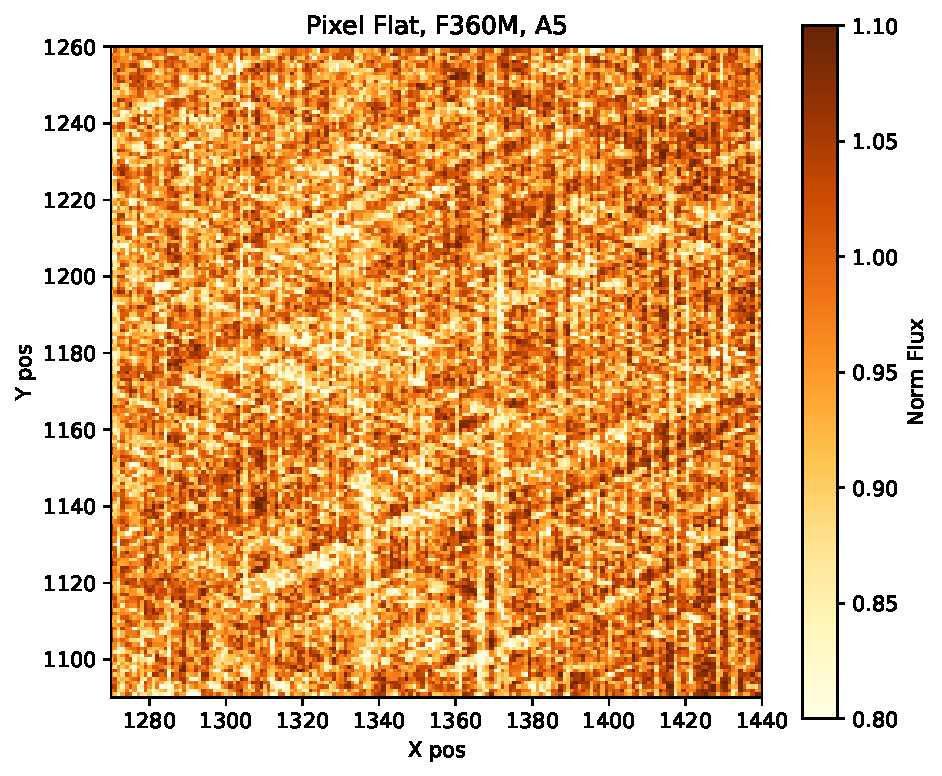
\includegraphics[width=.49\columnwidth]{crosshatch_zoom.pdf}
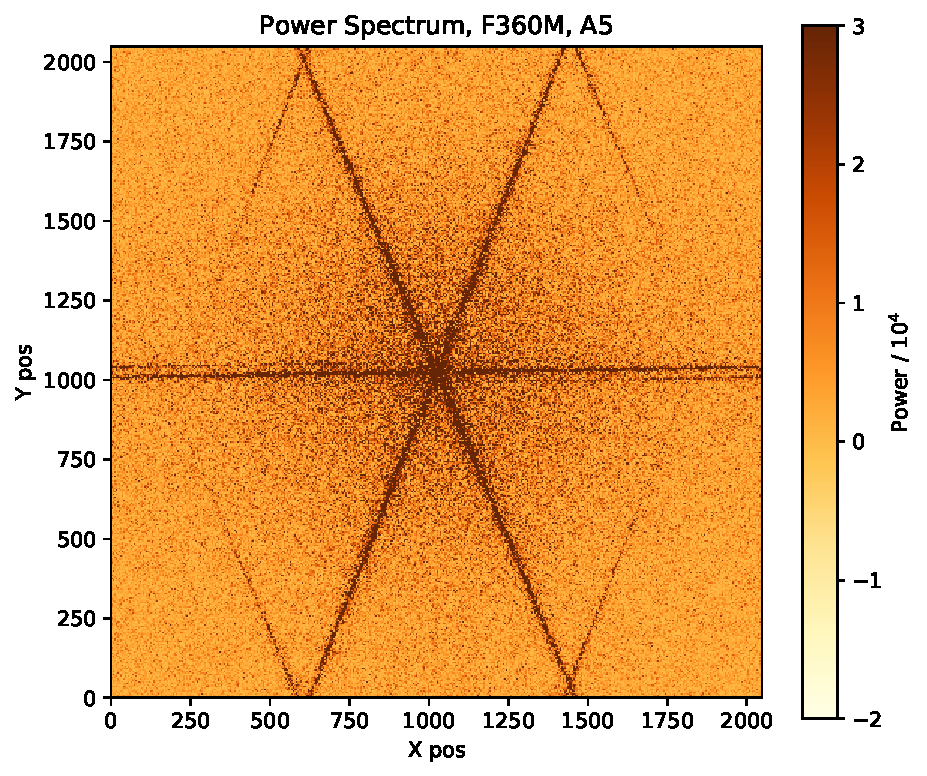
\includegraphics[width=.49\columnwidth]{crosshatch_2d_power.pdf}
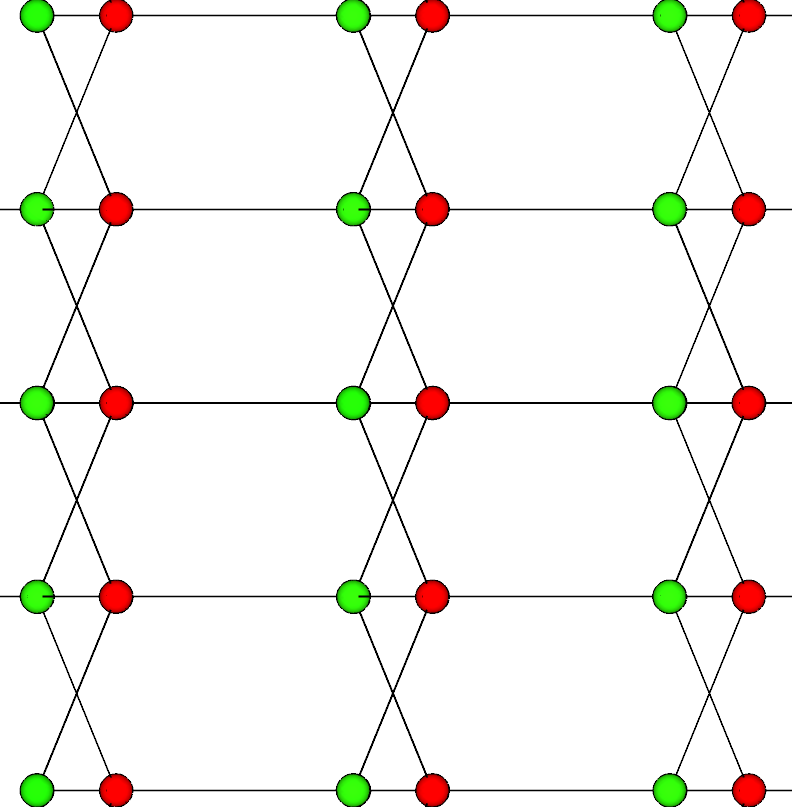
\includegraphics[width=.3\columnwidth]{tetrahedral_lattice_projection.png}
\caption{
The A5 detector's flat field has a pronounced crosshatch pattern at 23.1$\degree$ , 90.9$\degree$, and 158.6 $\degree$ CCW from the positive X direction.
The crosshatch pattern is visible in a zoom-in of the pixel flat field (top left).
The 2D power spectrum of the flat field (top right) shows a continuum of frequencies aligned with the three crosshatch angles.
Note the lines in frequency plane are perpendicular to the crosshatch directions in the image plane.
These three relative crosshatch angles (67.8$\degree$, 67.7$\degree$ and 44.5$\degree$) are similar to a projection of a tetrahedral (zincblende) lattice structure of HgCdTe (bottom, 67.8$\degree$, 67.8$\degree$, 44.4$\degree$) onto the [211] miller plane.
}\label{fig:crossHatchA5}
\end{figure}

The crosshatch pattern is wavelength dependent, as seen in Figure \ref{fig:crossHatchWavelengthDep}, where the throughput variations are the largest for short wavelengths (resolving crystal structures) and smallest for the long wavelengths.
This is visible both in the throughput cross section of the flat field and the Fourier amplitude of the crosshatch as a function of wavelength.
We find a steeper wavelength dependence to the crosshatch pattern near 0.9$\degree$ from horizontal in the frequency domain or 0.9$\degree$ from vertical in the length domain.
%We also fit the crosshatch pattern.

\begin{figure}[!hbtp]
\centering
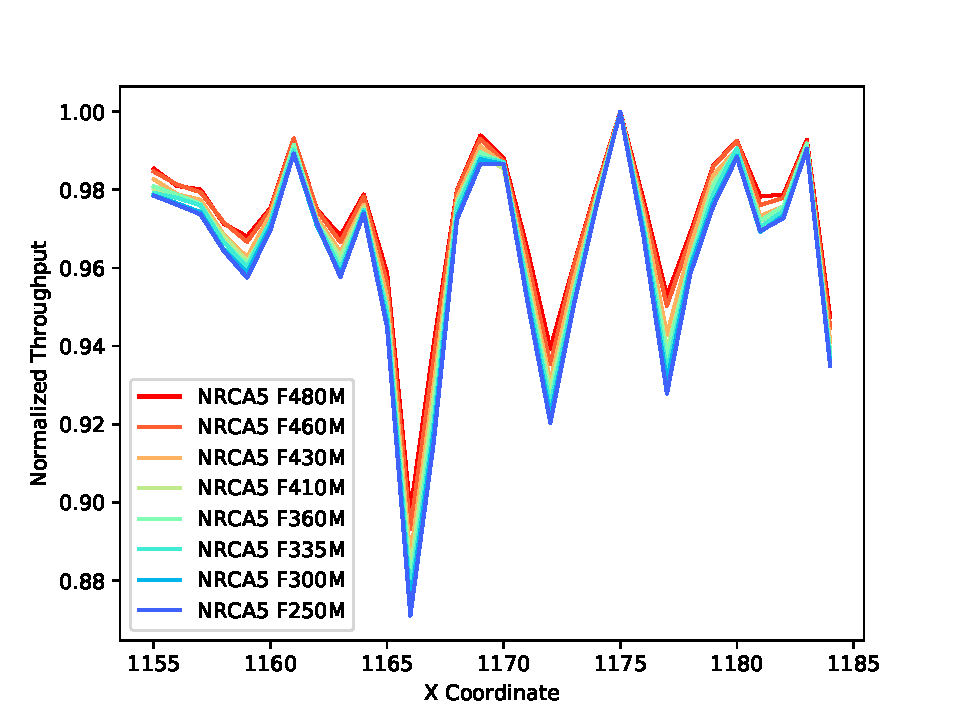
\includegraphics[width=.49\columnwidth]{cross_sec_of_crosshatch.pdf}
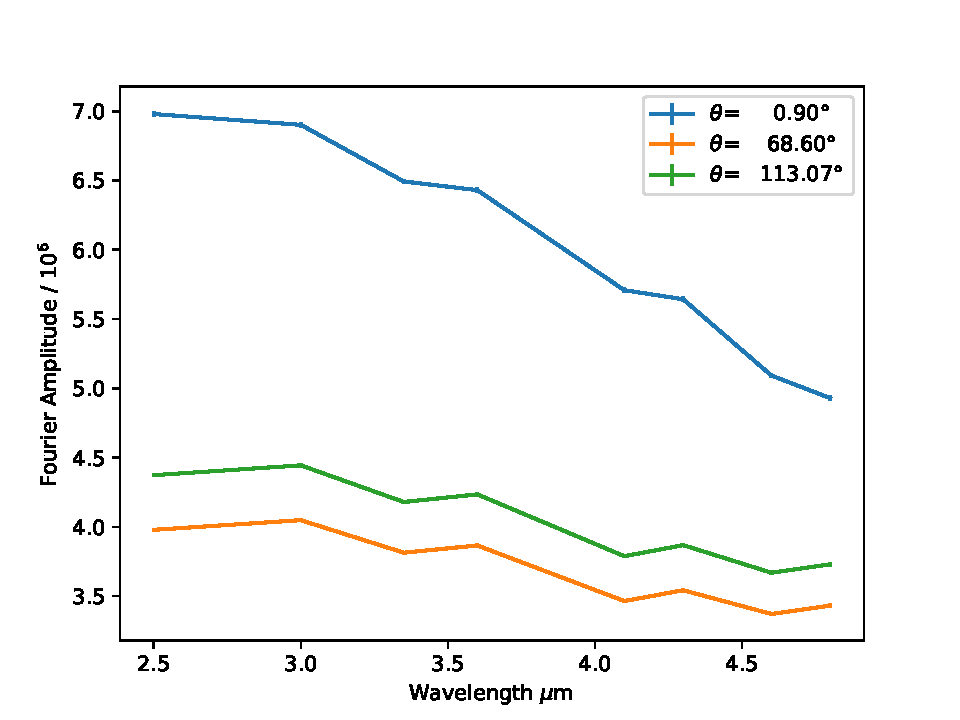
\includegraphics[width=.49\columnwidth]{fourier_power_from_fit.pdf}
\caption{
The crosshatch pattern changes as a function of wavelength, possibly because the shorter wavelengths resolve the structure better.
The shorter wavelengths have deeper crosshatch troughs (left) and higher Fourier amplitudes (right).
}\label{fig:crossHatchWavelengthDep}
\end{figure}


\subsubsection{Crosshatch Pattern Modeling}
We model the crosshatch pattern in the Fourier space because it has a smoother pattern as a function of spatial frequency than in spatial coordinates as seen in Figure \ref{fig:crossHatchA5}.
We divide the 2D Fourier power spectral density by the number of pixels in an input image.
This was experimentally determined to give a power spectral density that does not change with the dimensions of the input image.
\textcolor{red}{Can we justify this more?}

We model the two dimensional Fourier power spectral density $f(k_{x,i}',k_{y,i}')$ for one angle $\theta_i$ as
\begin{equation}\label{eq:analyticPSDradial}
f(k_{x,i}',k_{y,i}', a_i, b,c) = a_i \exp{\left(- |k_{x,i}'| / b \right)} \left( \frac{1}{(0.5 c)^2 + k_y'^2} \right),
\end{equation}
where $k_x'$ and $k_y'$ are rotated frequency coordinates in the parallel and perpendicular directions, $a$ is the amplitude, $b$ is the parallel exponential constant and $c$ is the Lorentzian full width at half maximum of the perpendicular dependence.
For each of the three angles, there is a set of rotated coordinates centered at $(k_{x,0},k_{y,0})$= (0,0) following:
\begin{equation}
k_x'(\theta_i) = k_x \cos{\theta_i} + k_y \sin{\theta_i}
\end{equation}
and
\begin{equation}
k_y'(\theta_i) = -k_x  \sin{\theta_i} + k_y \cos{\theta_i}.
\end{equation}
We include three angles so that the total power spectral density is
\begin{equation}
f(k_x,k_y) = \sum_{i=1}^{i=3} f_i(k_{x,i}'(\theta_i),k_{y,i}'(\theta_i),a_i,b,c) + d \exp{\left(-k_r/e_b\right)},
\end{equation}

This model has 8 free parameters: three angles ($\theta_i$, three amplitudes ($a_i$), a joint parallel exponential constant ($b$) and joint Lorentzian width ($c$).
Finally, we include an exponential term that fits the broad azimuthally symmetric background to all the power spectra,
where $d$ is the amplitude of the radial ``background'', $k_r= \sqrt{k_x^2+k_y^2}$ is the radial frequency and $e_b$ is the radial background exponential constant.
We only fit the region of the power spectral density above frequencies of 0.05 px$^{-1}$ to focus on the high frequency component of the flat field where the crosshatch is most prevalent.

For the F300M filter and ALONG detector, we find 
for $\theta_1 = 0.906 \pm 0.001 \degree, \theta_2 = 68.605 \pm 0.001 \degree, \theta_3 = 113.075 \pm 0.001, a_1 = 2.774 \pm 0.002 \times 10^{-7}, a_2 = 1.569 \pm 0.002 \times 10^{-7}, a_3 = 1.744 \pm 0.002 \times 10^{-7}, b=0.345 \pm 0.0005 $ px$^{-1}$, $c=2.05 \pm 0.07 \times 10^{-2}$ px$^{-1}$, $d=6.78 \pm 0.01 10^{-3}$ and $e_b=0.26 \pm 0.01$ px$^{-1}$.
The uncertainties were simply derived from the diagonals of the covariance matrix and likely are underestimated.

NIRCam's 10 SCA's have very similar crosshatch angles with separations of 44.5 $\degree$ and 67.7 to 67.8 $\degree$.
They tend to have one primary crosshatch axis oriented either along the X pixels or the Y pixels, with two flanking axes at $\sim 67.7 \degree$ to either side.
The long wavelength arrays have a more pronounced crosshatch than the short wavelength arrays.
The NRCB4 array's primary crosshatch direction is most closely aligned with a pixel axis (the Y direction) than any SCA.
Figure \ref{fig:crosshatchModelGallery} shows the best-fit crosshatch 2D power spectra.

\begin{figure}[!hbtp]
\centering
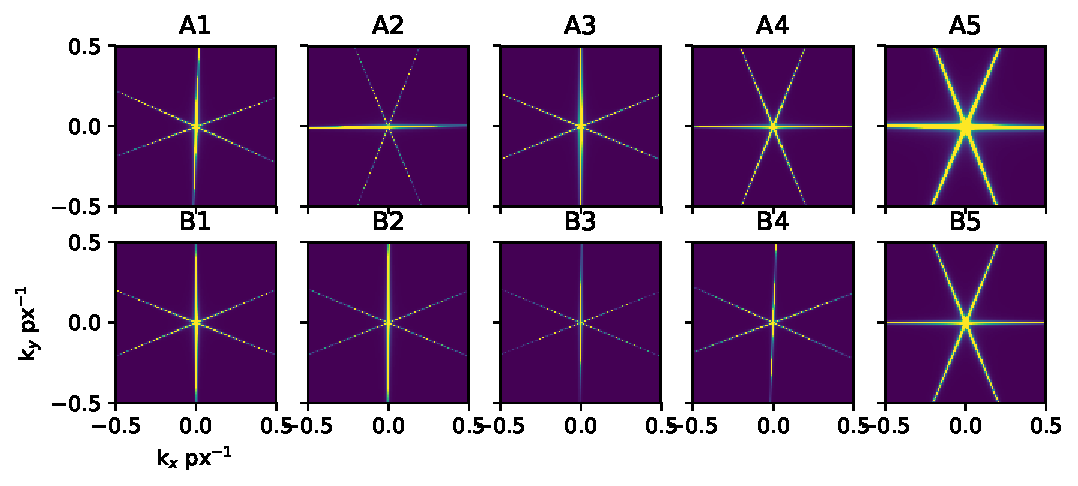
\includegraphics[width=.99\columnwidth]{psd_models_gallery.pdf}
\caption{
Best-fit power spectra of all the NIRCam detectors show that the long wavelength detectors A5 and B5 show the most pronounced crosshatch patterns.
The primary crosshatch tends to be aligned closely, but no exactly, with either the X or Y axis.
The images have all been normalized to the same scale to show the relative crosshatch amplitudes of different detectors.
}\label{fig:crosshatchModelGallery}
\end{figure}

\clearpage
\subsubsection{Position of SubGrism Array}

The crosshatch pattern varies in amplitude and angular dependence from one physical location on the detector to another.
The ALONG detector has more pronounced crosshatching toward the middle of the detector that falls off toward the perimeter.
On the other hand, the BLONG detector has more pronounced crosshatching towards the boundary.
We fit the crosshatch pattern to three regions of the ALONG detector, which is the one used for the NIRCam grism time series mode:
\begin{enumerate}
	\item The 2048$\times$64 SUBGRISM position at the bottom of the array where the bottom left corner is (4,5) \label{subgrism64pos}
	\item A 2048$\times$64 theoretical subarray at the top of the ALONG detector where the bottom left corner is (4,1984)
	\item A 2048$\times$64 cutout of the full frame detector that is centered on the grism time series field point.
\end{enumerate}

The three subarrays considered are shown in Figure \ref{fig:subpixScanSimulation}.
We exclude reference pixels (which form a 4 pixel wide boundary around the detector) and an additional row on the bottom and top of the array because these illuminated rows are outliers in the flat field.
The first position is nearly the same as the SUBGRISM64 subarray position in the grism time series mode, except that the SUBGRISM64 includes the first 5 rows which are excluded here from the crosshatch analysis.
The field point used for the SUBGRISM64 mode is expected to be the same one as will be used for the SUBGRISM128 and SUBGRISM256 subarrays.
The position at the top of the ALONG detector has the smallest amplitude of crosshatch pattern in all three directions.
The best-fit amplitudes are used as input to the jitter simulations in Section \ref{sec:CrosshatchSim}.
We find that the maximum flux change for a 0.1 pixel shift is 118 ppm for the nominal grism position, 108 ppm for the top of the array and 153 ppm at the full frame grism position.

\begin{figure}[!hbtp]
\centering
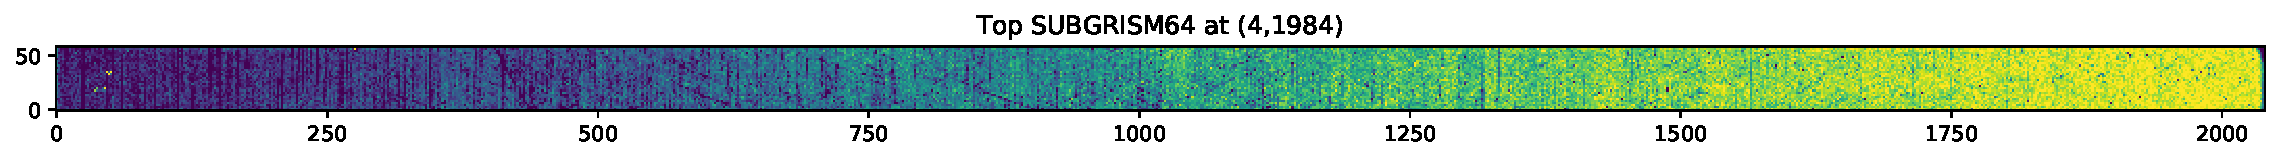
\includegraphics[width=0.99\columnwidth]{subg_pos_topGrism64.pdf}\\
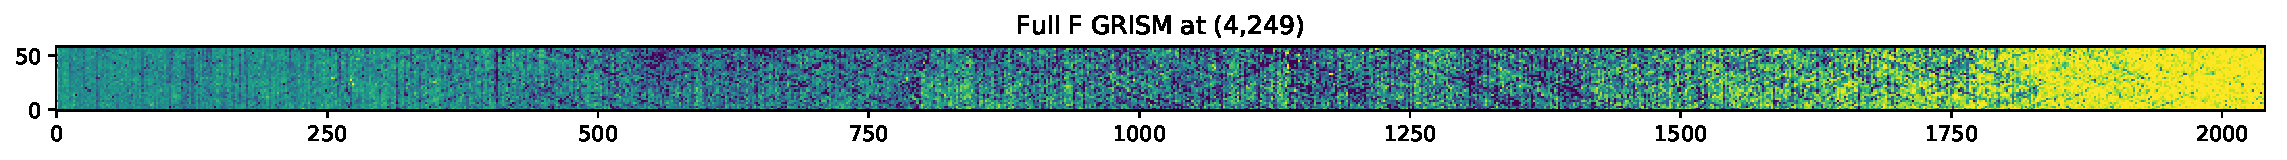
\includegraphics[width=0.99\columnwidth]{subg_pos_fullfGrismRegion.pdf}\\
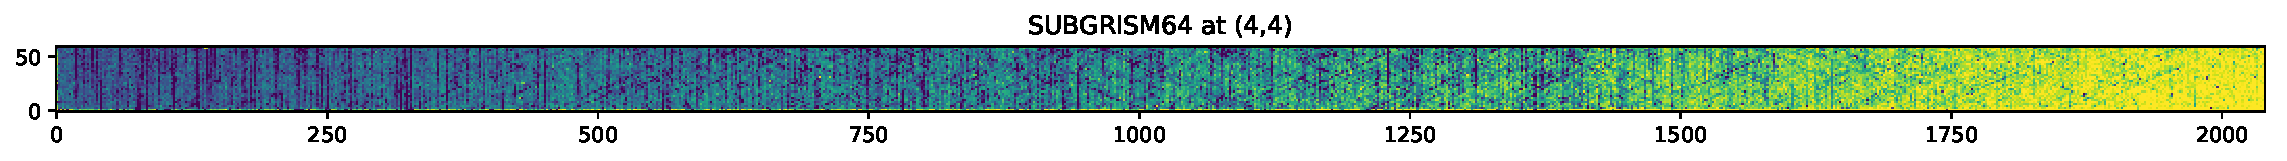
\includegraphics[width=0.99\columnwidth]{subg_pos_subgrism64.pdf}\\
\vspace{0.2in}
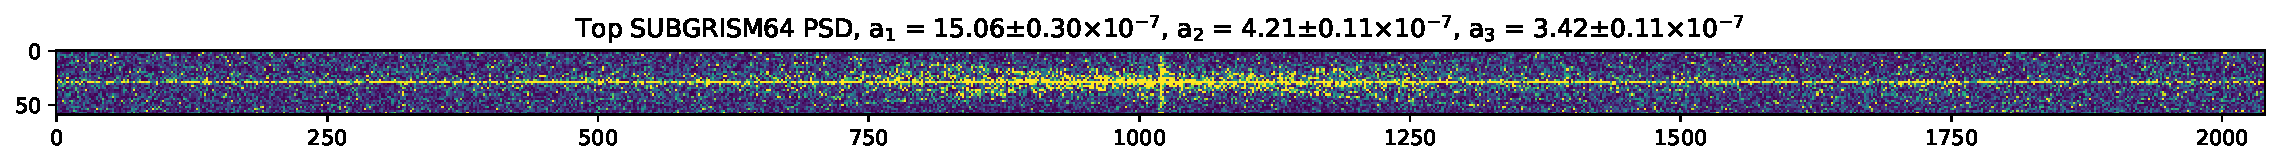
\includegraphics[width=0.99\columnwidth]{subg_pos_topGrism64_psd.pdf}\\
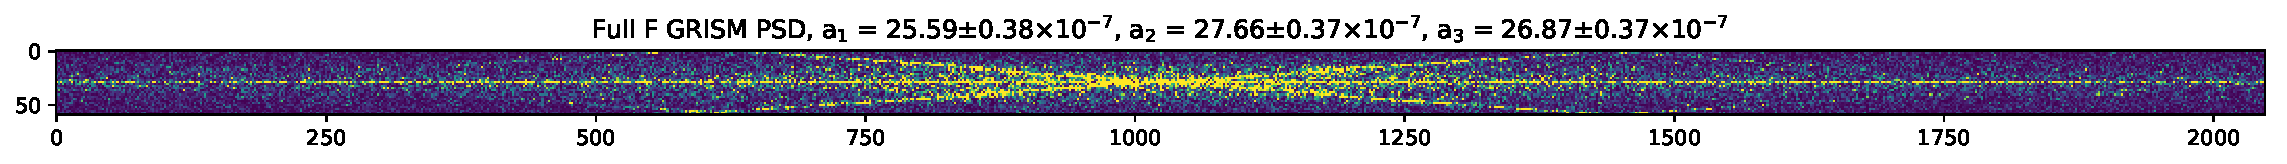
\includegraphics[width=0.99\columnwidth]{subg_pos_fullfGrismRegion_psd.pdf}\\
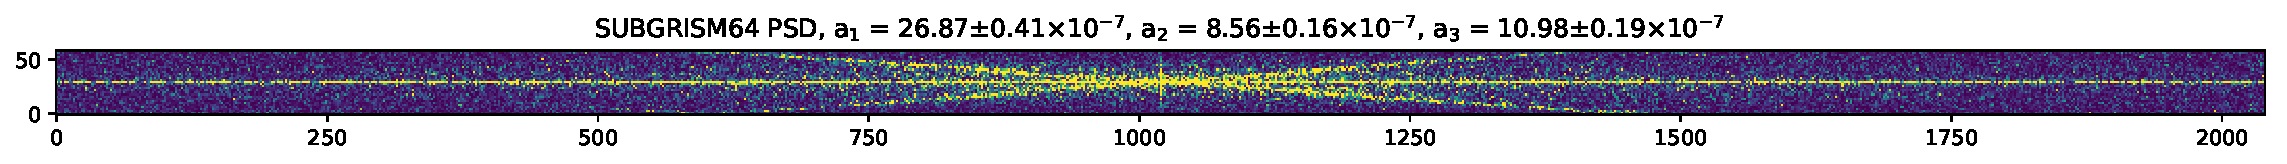
\includegraphics[width=0.99\columnwidth]{subg_pos_subgrism64_psd.pdf}\\
\caption{
The top of the array has the smallest level of crosshatching and the middle has the largest.
This is visible in the flat field images (top three panels) and their power spectral density functions (bottom three panels) for three different sections of the A5 detector: a theoretical ``aperture'' position at the top of the array (first plot from top), the full frame position near Y=512 (second plot from top) and the nominal SUBGRISM64 at the bottom of the array (third plot from top).
The bottom left corner for each subarray is listed in parentheses in the title of the flat field plot and the best-fit amplitudes are listed in the title of the power spectral density plot.
 }\label{fig:subpixScanSimulation}
\end{figure}

\subsubsection{Subpixel Crosshatching Calculation}\label{sec:CrosshatchSim}

The subpixel crosshatch pattern can potentially introduce time-variable noise as the point spread function drifts with telescope pointing drifts, long timescale jitter.
NIRCam observations are expected to have a root-mean-square deviation of 6.0 mas in each axis when measured in 15 second intervals over a 10,000 second observation.\footnote{See \url{https://jwst-docs.stsci.edu/display/JTI/JWST+Pointing+Performance\#JWSTPointingPerformance-Pointing\_stabilityPointingstability}}

We simulate the effect of this jitter on NIRCam time series observations with the following steps:
\begin{itemize}
	\item Fit the existing flat field to a crosshatch model in the Fourier domain
	\item Extrapolate the crosshatch model to higher frequencies (30 px$^{-1}$) to estimate the sub-pixel structure
	\item Simulate an over-sampled PSF using \texttt{webbpsf} \citep{perrin2014webbpsf}
	\item Multiply the PSF by the simulated flat field
	\item Scan the PSF along the X and Y directions up to a magnitude of 6 mas
	\item Bin the simulated images into the native pixel size
	\item Divide by the pixel-to-pixel flat field
	\item Measure the relative flux with a photometric aperture
\end{itemize}



We take the exponential model with best-fit parameters for the F300M filter and extend the exponential function out to an oversampling factor of 60 times the LW pixels.
We evaluate equation \ref{eq:analyticPSDradial} for frequencies in the oversampled image from 0 px$^{-1}$ to 30 px$^{-1}$ and multiply this by the number of pixels and the square of the oversampling factor (ie. $60^2$) to convert from the scale-invariant Power Spectral Density to the simulated PSD.
We then assign random phases uniformly from 0 to 2$\pi$ for the complex Fourier plane because the original image's complex phase distribution is similar to uniform.
Finally, we take the real part of the inverse Fourier transform to create an oversampled image, as shown in \ref{fig:crossHatchSimPSF}.
For comparison to the original flat in Figure \ref{fig:crossHatchA5}, we binned to the oversampled flat field to the native LW pixel (1.0 native pixels=60.0 oversampled pixels $\approx$0.063 \arcsec).
This simulated pixel flat field with dimensions of 26 by 26 LW pixels has a peak of 1.15 to trough of 0.90 with a robust standard deviation of 0.05.
For comparison, the middle of the original F300M flat for the ALONG detector has a robust standard deviation 0.06.

\begin{figure}[!hbtp]
\centering
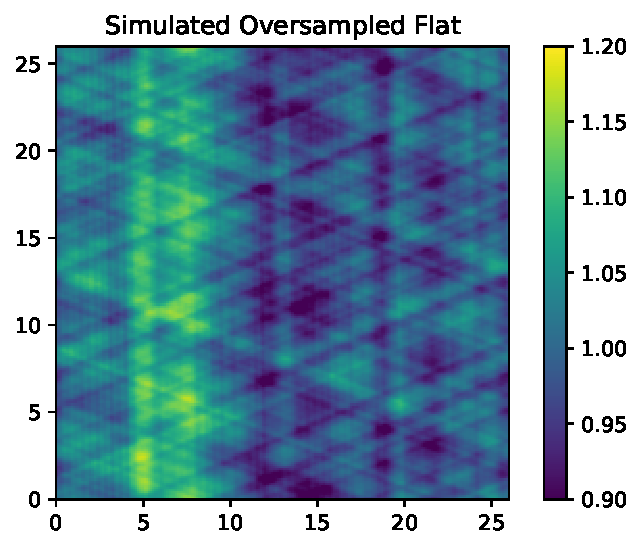
\includegraphics[width=.32\columnwidth]{sim_flat_Oversampled_plot.pdf}
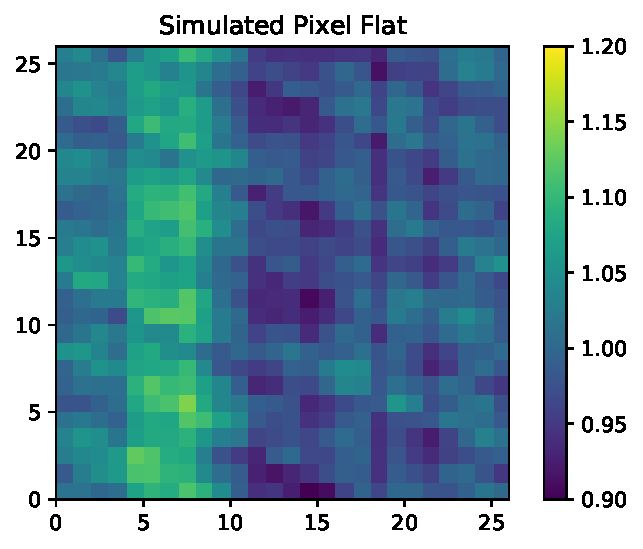
\includegraphics[width=.32\columnwidth]{sim_flat_Pixel_plot.pdf}
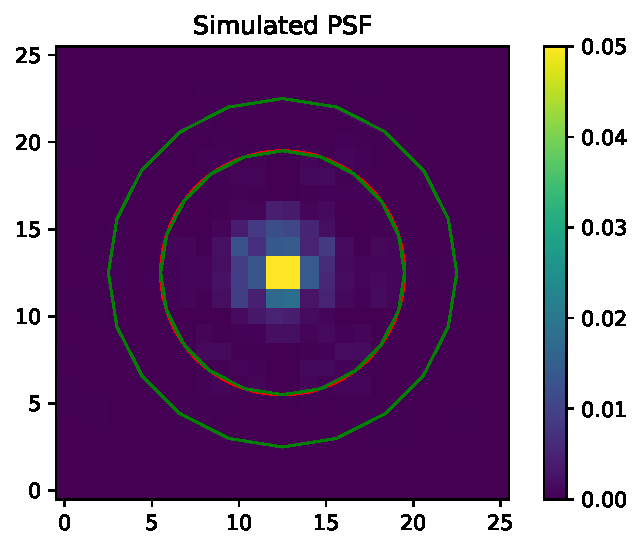
\includegraphics[width=.32\columnwidth]{psf_with_phot_ap_with_crosshatch.pdf}
\caption{
The steps of the sub-pixel crosshatch photometry simulation are shown here.
We simulate an over-sampled flat (left) by extrapolating the power spectrum to frequencies above the pixel sampling level.
This simulated flat is binned to the native pixel resolution to produce a pixel flat field (middle) that would be used by a standard pipeline that has no sub-pixel corrections.
A \texttt{WebbPSF} point spread function is created at the oversampled resolution, multiplied by the oversampled flat field and then binned to native resolution (right).
Finally, the simulated image is divided by the pixel flat field as would be performed in a standard pipeline reduction.
The simulated PSF shows the source and background apertures used in the simulation, which are centered on the PSF.
}\label{fig:crossHatchSimPSF}
\end{figure}

We next calculate a point spread function using \texttt{webbpsf} \citep{perrin2014webbpsf}, oversampled by a factor of 60.
\texttt{webbpsf} includes an optional blurring due to high frequency pointing jitter.
We set this Gaussian blurring parameter to 1 mas to simulate a worst-case scenario where the pointing drift is dominated by long-timescale behavior with minimal high frequency jitter.
We multiply the oversampled \texttt{webbpsf} source by the simulated oversampled flat and bin this to native pixel resolution to create a simulated observation as shown in Figure \ref{fig:crossHatchSimPSF}.
This simulated observation is divided by the binned simulated flat as would be done by a standard pipeline's flat field correction.

We repeat the last steps of the observation simulation by shifting the over-sampled PSF by sub-pixel amounts.
The subpixel shifts of the over-sampled PSF are performed with \texttt{scipy.ndimage.shift}.
For each shifted PSF, we multiply this by the subpixel crosshatch pattern and bin the result.
These simulated operations represent pointing drift on the subpixel scale.

We calculate aperture photometry with a circular aperture with a radius of 7 pixels and a background annulus from 7 to 10 pixels on each of the observations.
The aperture is re-centered by the same position as the shift direction.
For each sub-pixel pointing drift, the aperture sum is subtracted by the background flux average per pixel multiplied by the pixel area of the source aperture.
While the simulations here include no background flux, we use the background subtraction to simulate the operations applied by a photometry pipeline.
The differential flux between the centered PSF and the shifted one is shown in Figure \ref{fig:subpixScanSimulation}.


\begin{figure}[!hbtp]
\centering
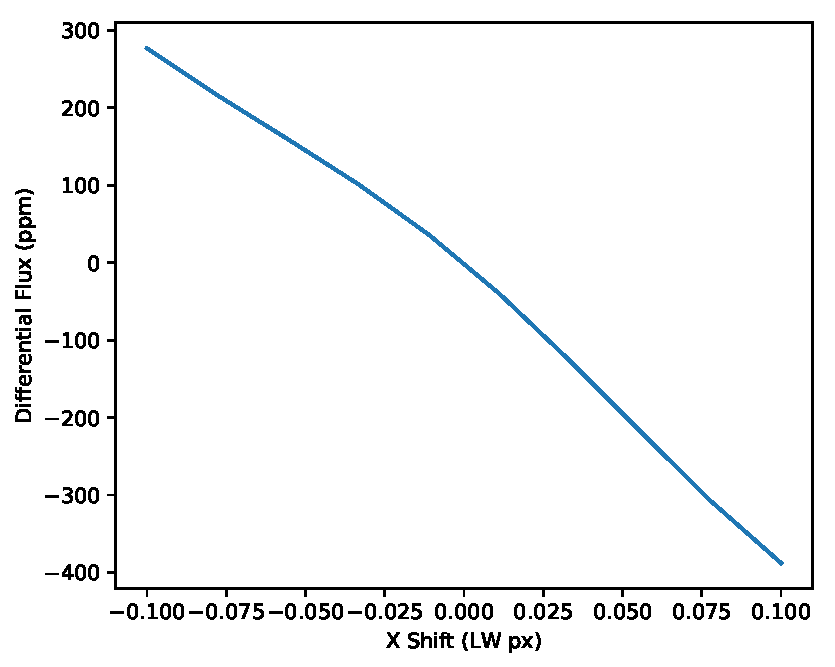
\includegraphics[width=.49\columnwidth]{scan_F300M_x_short_scan.pdf}
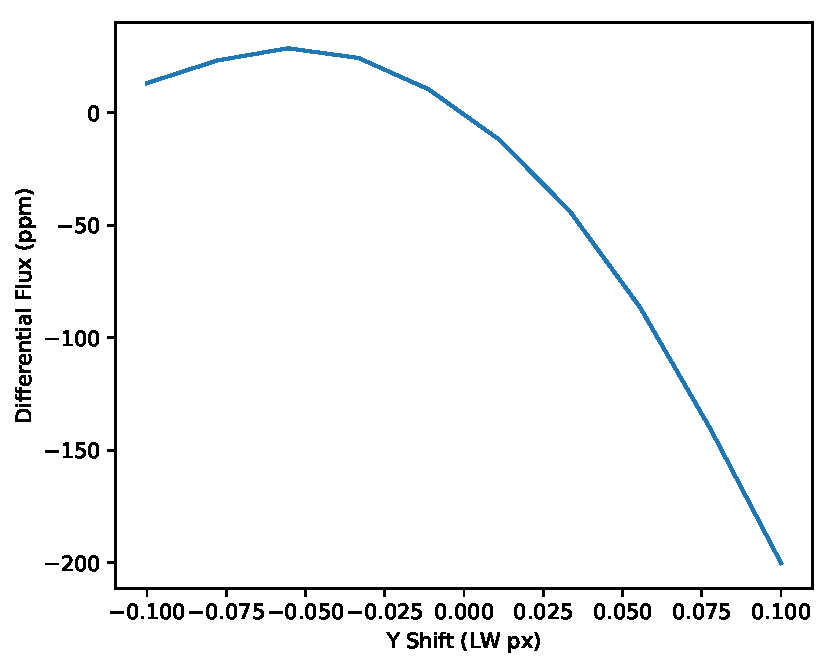
\includegraphics[width=.49\columnwidth]{scan_F300M_y_short_scan.pdf}
\caption{
The simulated subpixel crosshatch pattern from Figure \ref{fig:crossHatchSimPSF} for the F300M filter will cause spurious flux changes with small pointing drifts.
Here we show scans in the X direction and Y direction from the center of the image and a subpixel scale.
The amplitude of these scans is 6.3 mas for the $\sim$63 mas/px plate scale of the LW detector.
These are correctable with smooth functions such as polynomials.
}\label{fig:subpixScanSimulation}
\end{figure}

The subpixel crosshatch structure does indeed create flux variations with image motion as shown in Figure \ref{fig:subpixScanSimulation}.
The amplitude of the flux changes is potentially up to 300 ppm.
This is significant when compared to atmospheric features of giant planets ($\lesssim$ 100 ppm) or the transit depth of an Earth-like planet transiting a sun-like star ($\lesssim$ 80 ppm).

Fortunately, the subpixel crosshatch systematic is a smooth function of pointing drift, shown in Figure \ref{fig:subpixScanSimulation}.
A polynomial function can be fit to this subpixel dependence then the centroid of each integration can be inserted as an argument to the function to provide a correction as a function of time.
Alternatively, a Gaussian process regression could be applied.
Centroiding is possible in imaging and spectroscopic modes using PSF fitting or cross-correlation.
When the LW grism time series mode is enabled, SW imaging data will automatically be collected simultaneously enabling the SW centroids to be used to track the motion of the dispersed grism image.
Furthermore, the pixels for time series modes can be characterized in detail because the will be re-used for all time series observations in a given mode.
Target acquisition is expected to achieve centroiding accuracy $\lesssim$ 10 mas ($\lesssim 6$ mas) for unsaturated target acquisition.\footnote{https://jwst-docs.stsci.edu/display/JTI/NIRCam+Time-Series+Imaging+Target+Acquisition}
This ensures that time series observations will reliably return to the same location within the same set of pixels with every visit.

\subsubsection{Time Series Simulation}
The JWST fine steering mirror (FSM) is designed to correct any telescope pointing errors that are not full corrected by the reaction wheels.
The JWST attitude control system team provided a simulation of the expected pointing performance shown in Figure \ref{fig:tserPointingFull}.

The dominant variations in the pointing in the simulation from Figure \ref{fig:tserPointingFull} are High Gain Antenna (HGA) moves.
These are moves are designed to keep the antenna pointing at ground-based antennas for telemetry or data download.
Fortunately, the errors due to HGA moves damp quickly on $\lesssim$ 1 minute e-folding timescales, as show in Figure \ref{fig:tserPointingZoom}.
This means that for 1 minute integrations, only about 1\% of integrations will be affected by HGA moves and the data for these moves could be discarded.
Other pointing errors can be caused by reaction wheel jitter, the MIRI cryocooler and fuel slosh in the fuel tanks.
The effect of the reaction wheels and MIRI cryocooler will be to blur the PSF over an integration since they are higher frequency $\gtrsim 1$ Hz.
Fuel slosh happens at the beginning of a visit after the telescope is slewed, but will dampen quickly on 100 second timescales.
Therefore, the largest contributor to pointing variations will likely be HGA moves and thermal inter-boresight motion.

\textcolor{red}{Once, we have thermal inter-boresight motion, show how this affects pointing/flux}

\begin{figure*}
\gridline{\fig{histos_v2_v3.pdf}{0.45\textwidth}{Pointing Histograms} 
\fig{tser_v2_v3_zoom_none.pdf}{0.45\textwidth}{Pointing Time Series} }
\caption{The typical pointing stability is expected to be extremely stable to within a standard deviation of 2.4 mas (0.04 long wavelength pixels).
This pointing model only shows the line of sight variations, not including thermal distortions or the high frequency ($>$1 Hz) jitter.
}\label{fig:tserPointingFull}
\end{figure*}

\begin{figure*}
\gridline{\fig{tser_v2_v3_zoom_1.pdf}{0.45\textwidth}{Pointing Series Zoom 1} 
\fig{tser_v2_v3_zoom_2.pdf}{0.45\textwidth}{Pointing Series Zoom 2} }
\caption{Occasional pointing errors are expected to be quickly corrected by the fine steering mirror.
}\label{fig:tserPointingZoom}
\end{figure*}

We simulate the change in flux as a function of position using our oversampled flat field, as in Figure \ref{fig:subpixScanSimulation}.
First, we bin the sub-pixel jitter time series into 1 minute time bins to represent 1 minute integrations, as shown in Figure \ref{fig:tserPointingAndFlux}.
We then use the positions to shift the PSF on the oversampled flat field as listed at the beginning of this section.
The resulting flux variations are very small compared to factors like the 1/f noise.
The standard deviation of the time series due to small line-of-sight telescope jitter on top of the subpixel crosshatching pattern is only 6 ppm.
Therefore, the line-of-sight subpixel jitter is expected to have a small affect on NIRCam stability.
Furthermore, centroid motion measurements can be used to correct the flux variations due to subpixel jitter with a polynomial or Gaussian process regression.

\begin{figure*}
\gridline{\fig{subpx_jitter_sim.pdf}{0.7\textwidth}{}}
\caption{The pointing time series from Figure \ref{fig:tserPointingFull} is binned into a 1 minute cadence and used as an input shifts to the crosshatch model.
The very precise pointing expected by JWST will produce very small flux variations on the crosshatch pattern with an expected standard deviation of only 6 ppm.
}\label{fig:tserPointingAndFlux}
\end{figure*}



\clearpage

\subsection{Random Telegraph Noise and RC pixels}
Several pixels exhibit RC (exponential) behavior and other exhibit unpredictable jumps in their DC levels.
The jumps are called Random Telegraph Noise (RTN) and some examples are shown in Figure \ref{fig:RTNandRC}.
These are rare events (400-1000 pixels out of 4$\times 10^6$) so they are unlikely to end up in a grism or in-focus aperture.

For Weak Lens photometric aperture (such as a 70 pixel radius aperture), there will be of order 2-4 pixels exhibiting RTN.
The RTN may not be removed by jump detection algorithms if they are similar order of magnitude to the photon noise for a single pixel ($\sim$180 DN).
If these are not identified, the RTN can contribute $\sim$200 counts in 4$\times 10^7$ or 5 ppm changes.

There are also RC pixels (as shown in Figure \ref{fig:RTNandRC}) that have exponential curves like a resister-capacitor circuit.
These pixels consistently show RC behavior and are flagged as ``Do-not-use'' for the pipeline so they may be skipped in the aperture summation.
There are 15 RC pixels in a 20 pixel tall F444W aperture and 31 RC pixels in a 20 pixel tall F322W2 aperture.

\begin{figure*}
\gridline{\fig{example_rtn.pdf}{0.45\textwidth}{RTN Pixels} 
\fig{{example_rc.pdf}}{0.45\textwidth}{RC pixels}}
\caption{Pixels sometimes exhibit unusual behaviors that are not related to counting photon flux.
Examples are shown for RTN and RC pixels.
}\label{fig:RTNandRC}
\end{figure*}


\clearpage
\section{Ground-based Experiments}\label{sec:experiments}

Table \ref{tab:testSummary} contains a summary of the ground-based tests that were performed on NIRCam detectors.
The flight NIRCam detectors, controllers, electronics, optics and instrument hardware were used in the Cryogenic Vacuum 3 (CV3) Test 3 as well as OTIS (Optical Telescope Element and Integrated Science).
There are also dewars at the Steward Observatory at the University of Arizona used for time series stability tests.
The GL dewar experiments used flight-like detectors, but a different controller (Leach).
The Asic dewar located at Steward Observatory in Tucson, Arizona used the same kind of detectors as NIRCam, the same kind of asic controllers and the same flight software, but no flight-like optics.
These two different kinds of detector electronics can be compared against each other to help isolate optical-related systematics, detector-related systematics and electronics-related systematics.

The instrument modes tested included mostly imaging with narrowband LEDs, but there was also a test with spectroscopy on a broadband source.
The one test with a broadband source was an OTIS stability test at NASA Johnson was a grism spectroscopy mode, which illuminated the long wavelength detector with a slitless spectrum covering 2.4 to 4.0~$\mu$m for the F322W2 filter, as seen in Figure \ref{fig:ampOffsetsOtisGrismSlope}.
The WLP8 imaging tests are where a point source is de-focused by 8 waves with a weak lens (WLP8), as shown in Figure \ref{fig:WLP8PSF}.
This mode was designed for wavefront sensing, but is also useful for high-precision time series because it spreads the light over many pixels.
The weak lens produces a point spread function (PSF) that is hexagonal like JWST's mirrors and has a flat-to-flat width of $\sim$108 pixels and a vertex-to-vertex width of $\sim$136 pixels.
The hexagonal PSF also has a central vertical peak which can be used for aperture centering.
The tests with the GL and ASIC dewars did not have NIRCam optics and instead were flood illuminated with a light source that had large spatial variations due to a non-uniform source.
 
\begin{deluxetable*}{ccCrlcc}[b!]
\tablecaption{Summary of Ground-Based Tests}\label{tab:testSummary}
\tabletypesize{\footnotesize}
%\tablecolumns{7}
%\tablenum{2}
\tablewidth{0pt}
\tablehead{
\colhead{Name} &
\colhead{Location} &
\colhead{Test Year} &
\colhead{Best Stability} & 
\colhead{Light Source} & 
\colhead{Instrument Mode} &
\colhead{Flight Hardware?} \\
\colhead{} &
\colhead{} &
\colhead{(YYYY)} &
\colhead{(ppm)} &
\colhead{} &
\colhead{} &
\colhead{}
}
\startdata
%Lockheed CV& Lockheed Martin& 2014??    & \nodata   & Darks         & Long Darks & \nodata \\ 
%Reset per int test & Lockheed Martin& 2014??    & \nodata   & Darks         & Long Darks & Y \\ 
CV 3       & NASA Goddard  & 2016       & 500   	& LED           & WLP8 imaging & Y\\
OTIS       & NASA Johnson  & 2017       &   2200    	& Continuum     & Grism spectroscopy & Y\\
OTIS       & NASA Johnson  & 2017       &   21,000    	& Continuum     & WLP8 Imaging & Y \\
GL dewar   & Steward Obs.  & 2015-2016  &       	& LED	        & flood-illuminated imaging & N \\
Asic dewar & Steward Obs.  & 2017-2019  &       	& LED           & pinhole \& flood-illuminated imaging & N\\
\enddata
\tablecomments{Cryogenic vacuum (CV), Optical Telescope element and Integrated Science (OTIS).}
\end{deluxetable*}

\clearpage
\subsection{OTIS Long Darks}\label{sec:longDarks}

It is instructive to look at dark frames to isolate the contributions of the read-out electronics, including the side-car asic, and how much they contribute to the error budget.
The dark frames do not have issues with the photometric stability of illumination lamps, which is a persistent challenge with ground-based tests.
They also do not contain photon noise in the background, which can mask the electronic noise sources.
We study here the contributions from read noise, 1/f noise and dark current.
This experiment with dark frames does not test subtle changes in behavior of the electronic read noise under illumination, such as cross-talk where pixels that have no direct flux from a source in an image correlate with other regions of the detector with high flux rates.

A standard long dark exposure used for detector characterization is a single integration that is 108 groups of 1 frame each (RAPID mode).
The detectors are read in full frame mode so that each frame is 10.7 sec in duration with 4 output amplifiers in use, thus the total time for the exposure is 19.3 min.
We use one of these long dark integrations to create simulated time series as if it were observing many consecutive integrations in full frame mode.
The long darks are broken into 54 sequential pairs of images that are subtracted from each other (integration 1 minus integration 0, 3 minus 2, 5 minus 4 etc. in a zero-based counting scheme).
Figure \ref{fig:longDarkPhot} shows an example dark read pair from frame 55 minus frame 54.
In the raw data, there are 4 prominent vertical stripes that are 512 pixels wide and 2048 pixels tall due to offsets in the read-out amplifiers.
These amplifier offsets are caused by drifts in the reference voltage that are reset once per frame and vary from amplifier to amplifier.
Additionally, there are obvious correlations along the fast-read (X) direction due to 1/f noise that appear as horizontal stripes in the image.

The ramps-to-slope pipeline \texttt{ncdhas} or the STScI JWST pipeline will apply reference pixel correction, bad pixels masks and non-linearity correction before fitting the groups up the ramp to a line.
In this work, we use \texttt{ncdhas}.
As seen in Figure \ref{fig:longDarkPhot}, reference pixels can be used to reduce the large offsets between amplifiers.
The reference pixels (making up a 4 pixel boundary on the edges of the detector) are un-illuminated and can therefore be used to measure common-mode electronic noise without being affected by photon counting noise.
The reference pixels are most useful for subtracting the offsets between amplifiers because there are 8 rows of 512 pixels or a total of 4096 reference pixels to average for each amplifier at the bottom and top of the arrays.
There are an additional 4 columns on the left and right side boundaries (8176 pixels) that can be used to further correct the left and right amplifier offests.
However, the 1/f noise that correlates along the fast-read (X) direction is more difficult to remove with reference pixels.
Only 4 pixels on the left and 4 pixels on the right side may be used to subtract the 1/f noise in a given row and the 4 amplifiers can exhibit different 1/f noise. 
Therefore, significantly residuals remain along the fast-read (X) direction in the reference-corrected read pair shown in Figure \ref{fig:longDarkPhot}.
These side reference pixels also cannot give any information about the read noise correlations that happen on shorter length scales than 512 pixels (5 ms).

\begin{figure*}[!hbtp]
\centering
\includegraphics[width=.32\columnwidth]{ap_labels_dark_NRCALONG-DARK-7235074213_1.pdf}
\includegraphics[width=.32\columnwidth]{ap_labels_darkRed_NRCALONG-DARK-7235074213_1.pdf}
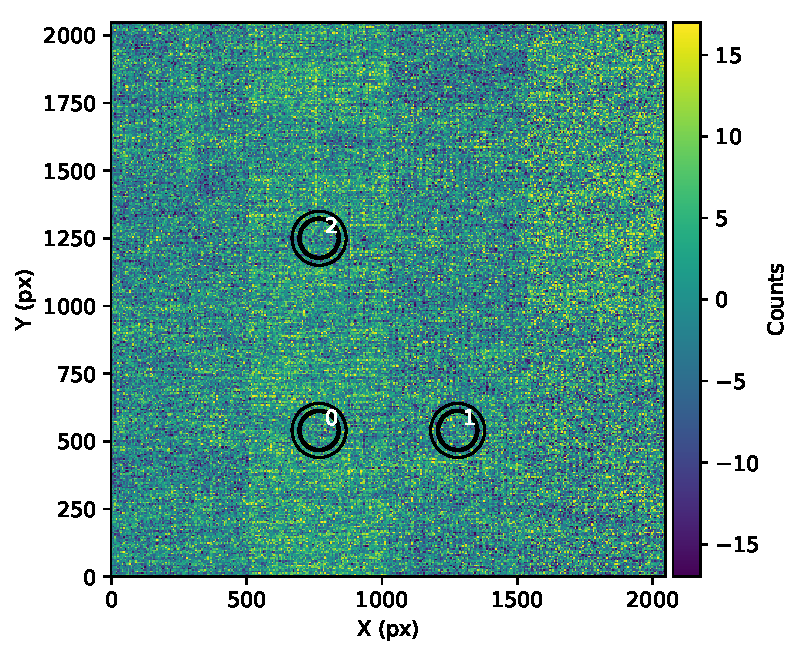
\includegraphics[width=.32\columnwidth]{ap_labels_row_by_row_group_sub_aps_1_NRCALONG-DARK-7235074213_1.pdf}
\includegraphics[width=.32\columnwidth]{long_dark_dark.pdf}
\includegraphics[width=.32\columnwidth]{long_dark_darkRed.pdf}
\includegraphics[width=.32\columnwidth]{long_dark_darkRedRowSub.pdf}
\caption{Time series of a 70 pixel radius photometric aperture obtained during a long dark exposure for detector ALONG=A5. The long dark exposure of 108 frames is used to construct 54 pairs of reads that are subtracted, in analogy with a series of integrations.
{\it Top:}  Example read pair subtraction with an overlay of the apertures for 3 different reduction steps from ``Raw" data using no reference pixel correction, ``Reduced Data" using reference pixels and ``ReducedRowColSub" using reference pixels and background subtraction for each row and each column.
{\it Bottom} The time series for each circular aperture with background subtraction using a circular annulus.
The most important step for reducing the noise in the time series is row-by-row subtraction to remove the 1/f noise.
}\label{fig:longDarkPhot}
\end{figure*}

What is most useful for exoplanet transit measurements is the photometric stability within an aperture or spectrum.
We therefore perform aperture photometry on the dark frame as if it were a weak lens image with a 70 pixel radius circular source aperture and a 75 to 100 pixel background annulus illustrated in Figure \ref{fig:longDarkPhot}.
Also, Figure \ref{fig:WLP8PSF} shows an example weak lens PSF with this aperture.
The background subtraction will largely remove the offsets affecting the whole 512$\times$2048 amplifier.
However, the correlated 1/f noise along the X direction will not be subtracted efficiently by an annulus.
Instead, a row-by-row line fit to the background would be more effective.

For a read pair subtraction, the ``CDS'' (correlated double sample) read noise is 13.3 e$^-$ or 7.2 DN for the A5 detector studied here.
If we assume each pixel's read noise is uncorrelated with its neighbors, the total noise within the source aperture is then $\sqrt{N_{px}} \times RN $ where $N_{px}$ is the number of pixels and $RN$ is the read noise of a single pixel.
If we also assume that the background pixels are uncorrelated with each other and the source pixels, then the total noise in background-subtracted photometry is 1310 DN.

This theoretical read noise should be compared to the photon noise expected inside an aperture during photometric stability time series applications.
The number of DN collected within a 70 pixel radius aperture for WLP8 data in our CV3 detector stability test with 2 groups in RAPID (ie a correlated double sample) was $S_{tot}=3.9\times 10^7$ DN during the integration.
The peak pixel counts in this integration were 30,000 DN or about 60\% well depth for the A1 detector.
The Poisson shot noise for photons is $N_{phot} = \sqrt{S_{tot}} / \sqrt{G} = 4,400$ DN, where $G$ is the gain ($G \approx 2.0$ for the SW detectors).
In terms of fractional noise, the photon shot noise should be 113 ppm and the read noise should be 33 ppm.
Therefore, the read noise is expected to be 1/4 the shot noise for 2 group RAPID read mode (ie CDS).
When averaging together 111 full frames over 60 minutes (an order-of-magnitude transit duration for most planets), the photon noise would contribute 11 ppm and the read noise would contribute 3 ppm.

In our experimental time series, however, the standard deviation in the time series in these 3 apertures is 22,000 to 25,000 DN (without any attempt to correct for 1/f noise using reference pixels or otherwise).
If uncorrected, this extra read noise will contribute 560 to 630 ppm to the time series per read pair!
This read noise would be $\sim$5$\times$ the $\sim$113 ppm photon noise.
Fortunately, there are ways to significantly reduce the 1/f noise.

\begin{deluxetable*}{c|cc|cc}[b!]
\tablecaption{Summary of Noise Sources in OTIS Dark Test}\label{tab:noiseSummaryWLP8}
\tabletypesize{\footnotesize}
%\tablecolumns{7}
%\tablenum{2}
\tablewidth{0pt}
\tablehead{
\colhead{Aperture} &
\multicolumn{2}{c}{WLP8} &
\multicolumn{2}{c}{Grism 0.17 $\mu$m bin}\\
\colhead{Noise Description} &
\colhead{$\sigma$} &
\colhead{$\sigma$} &
\colhead{$\sigma$} &
\colhead{$\sigma$} \\
\colhead{} &
\colhead{DN} &
\colhead{ppm} &
\colhead{DN} &
\colhead{ppm}\\}
\startdata
Ideal Photon Noise & 4,400 & 113 & 1,520 & 364 \\
Ideal Uncorrelated Read Noise & 1,300 & 33 & 470 & 113 \\
\hline
Measured Read Noise with amplifier offsets (no correction) & 23,500 & 600 & 81,220 & 19,450  \\
Measured Read Noise (reference pixel correction) & 10,800 & 280 & 12,900 & 3,090 \\
Measured Read Noise (reference channel subtraction) & 9,700 & 250 & & \\
Measured Read Noise (row-by-row subtraction) & 6,000 & 150 & 7,120 & 1,705 \\
Measured Read Noise (20 Component PCA subtraction) & 5,400 & 140 & & \\
Measured Read Noise (smoothed 161 px kernel interpolating over aperture) & 3,300 & 85 & & \\
Measured Read Noise (5 Component PCA on each amplifier) & 3,200 & 81 & & \\
Measured Read Noise (row-by-row amp-by-amp mean subtraction) & 2,900 & 75 & & \\
Measured Read Noise (smoothed 40 px kernel on top of aperture) & 900 & 23 & & \\
\enddata
\tablecomments{The theoretical and measured noise sources in one integration for a Weak Lens +8 and Grism Time Series.
The ppm units are assuming a peak 60\% well depth or 3.9$\times 10^7$ DN during an integration for the weak lens PSF and 4.2$\times 10^6$ DN during and integration for the grism PSF.
The noise is the sum within a 70 pixel radius source aperture and 75 to 100 pixel background aperture (in DN) or relative to the photon signal (in ppm).
The integration is assumed to be a bright source with 2 groups of 1 integration each up the ramp (Correlated Double Sampling or CDS mode).}
\end{deluxetable*}

These large correlations in read noise can be reduced with the side reference pixels, which are designed to track electronic noise without the presence of background photon noise.
We use the \texttt{ncdhas} pipeline to apply reference pixel correction, which dramatically reduces the amplifier offsets and also reduces 1/f noise correlations along the fast read (X) direction.
The time series for the 3 apertures considered drops down to 10,000 DN to 11,500 DN, but still falls short of the expectation of 1,310 DN if the read noise is uncorrelated.

Since these 8 reference pixels in each row are not sufficient to remove all 1/f noise in each row, so we perform another correction step:
We find the median of each group up the ramp along the fast read (X) direction and subtract this from every row.
This amounts to a row-by-row background subtraction.

In the latter case, the standard deviation of the time series drops to 6000 DN, but is still larger than the expectation of 1310 DN of all noise were uncorrelated.
The A3 detector used for weak lens photometry has reduced 1/f noise.
The standard deviation of the raw time series is 15,000 compared with the 22,000 from the A5 (ALONG) detector.

\subsubsection{Mean Row by Amplifier}\label{sec:indAmpAvg}
A slight modification to the above strategy is to average each amplifier individually.
This takes care of any differences between amplifiers.
This individual amplifier dramatically decreases the errors.
The standard deviations of the background-subtracted photometry range from 2,540 to 3,300 DN or 65 to 85 ppm.
Therefore, this simple approach can dramatically decrease the 1/f noise to below the photon limit.
This is possible for Weak Lens photometry but not grism spectroscopy when dispersed parallel to detector rows (the fast-read direction).

\subsubsection{Smoothed Kernel Subtraction}\label{sec:smoothKernelSub}

We also consider more effective ways to reduce read noise than the median row subtraction discussed in Section \ref{sec:longDarks}.
We start by applying a smoothing kernel to each group (1 read for RAPID mode) up the ramp of the raw data.
The kernel is a uniform normalized kernel 1 pixel in height and 40 pixels along a row.
This enables subtraction of 1/f noise that has length scales shorter than the row length (ie timescales shorter than 5 milliseconds, which the median subtraction cannot remove.

This smoothing kernel makes a dramatic improvement to the final weak lens aperture time series, as shown in Figure \ref{fig:longDarkWithRowKernel}.
The standard deviation in the time series drops from the best previous method (row and column median subtraction) by a factor of nearly 10!
For the row and column median subtraction applied to the red files, the standard deviation was 6150, 5600 and 6,600 DN for apertures 0, 1 and 2.
For the same apertures, the standard deviation in the time series drops to 650, 890 and 570 DN.

\begin{figure*}[!hbtp]
\centering
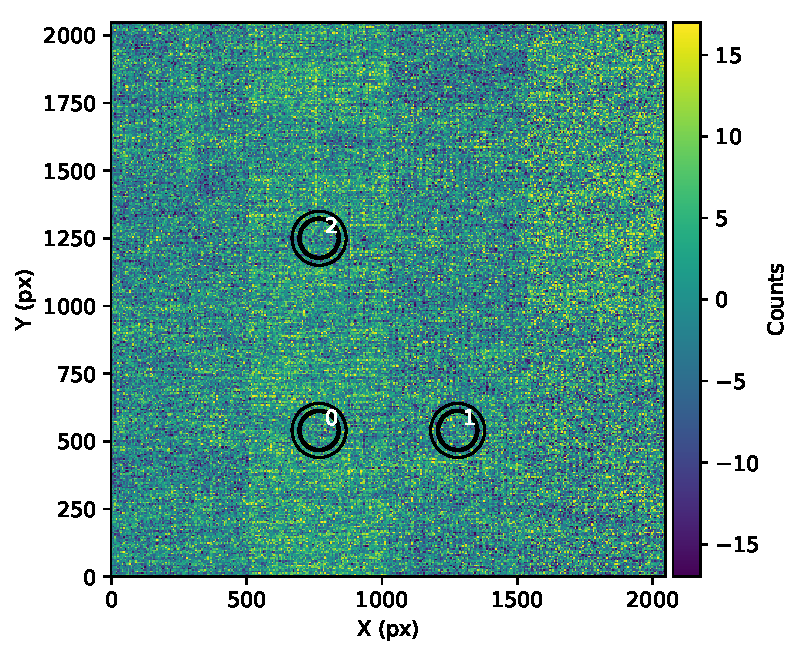
\includegraphics[width=.37\columnwidth]{ap_labels_row_by_row_group_sub_aps_1_NRCALONG-DARK-7235074213_1}
\includegraphics[width=.37\columnwidth]{ap_labels_darkRedsmoothedRowKernel_NRCALONG-DARK-7235074213_1.pdf}
\includegraphics[width=.37\columnwidth]{zoom_long_dark_row_by_row_group_sub.pdf}
\includegraphics[width=.37\columnwidth]{zoom_long_dark_darkRedsmoothedRowKernel.pdf}
\caption{The same apertures as Figure \ref{fig:longDarkPhot}, but with subtraction by a smoothed image where a 40 pixel wide and 1 pixel tall averaging kernel was applied along the fast read direction of every group.
Subtraction by the smoothed image has a dramatic effect on reducing correlated 1/f read noise from $\sim$6,000 DN to $\sim$700 DN in the aperture.
}\label{fig:longDarkWithRowKernel}
\end{figure*}

The dramatic difference from the smoothing kernel is beyond what is possible for a real source.
This is because the 40 pixel wide kernel was applied all the way through the source aperture, which would subtract and distort any signal from a star/planet source.
In reality, the kernel should be wider than the source aperture diameter and interpolate through the source points.
Note that this experiment would result in perfect subtraction (0 ppm noise) if the kernel was only 1 pixel wide!
We repeated the experiment with a 161 pixel wide kernel and masked bad pixels and the source pixels.
We use the \texttt{astropy.convolution.convolve()} routine, which calculates a convolution of the kernel by the image.
\texttt{astropy.convolution.convolve()} ignores al NaN values in the mask and renormalizes the kernel by the sum of the remaining kernel points.
This efficiently interpolates over bad pixels and can also interpolate over the source aperture.
Our smoothing kernel is a flat boxcar normalized to 1.0.
This more realistic kernel results in higher noise because of its larger window size and because it interpolates over the aperture points.
The resulting time series has a standard deviation of 2800 DN to 3700 ppm.
This is still larger than the 1,300 DN expectation for uncorrelated read noise, but is below the ideal photon noise limit when integrations reach 60\% well depth.

\textcolor{red}{\bf Continue Here!}

\subsubsection{Reference Channel Subtraction}
We note that the 4 channels can sometimes exhibit the same 1/f correlation behavior, as shown in Figure \ref{fig:darkPixelTimeSeries}.
Another option to remove 1/f noise is to subtract the illuminated amplifier with a target in it by un-illuminated channels.
We attempt to subtract an amplifier 0's time series from all amplifiers.
Of course, this means that this amplifier is perfectly subtracted and no noise or signal remains in this 1/4 of the image.
The subtraction step should increase the read noise on an individual pixel by $\sim \sqrt{2}$ because the errors from the subtracted pixel should add in quadrature to the original pixels.
This increase in read noise on a per-pixel level might be acceptable if it decreases the correlated errors along the rows.
On the other hand, if the each amplifier exhibits its own individual correlated noise behavior, the reference amplifier will fail to subtract out all correlated noise and may introduce more noise.

The net effect of this method is to increase the noise over a row-by-row median subtraction.
The standard deviations in the time series range from 8,500 DN to 10,800 DN for this reference amplifier method as opposed to the 5,500 DN to 6,600 DN for a row-by-row median.
This means the the correlations within an amplifier are not efficiently subtracted and may be propagated to the remaining amplifiers.

\begin{figure*}[!hbtp]
\centering
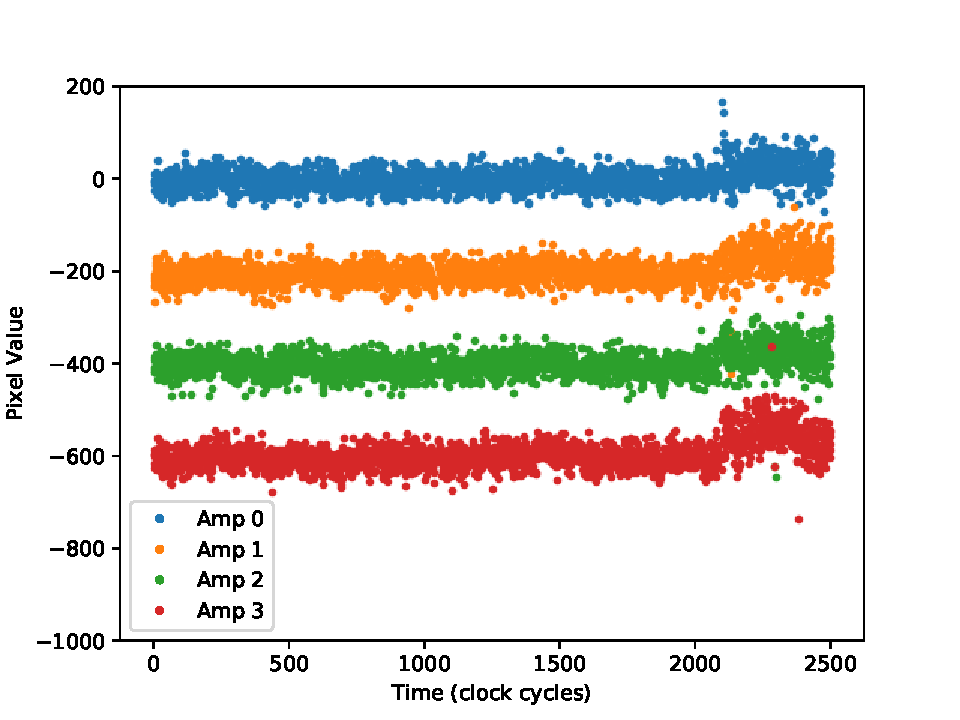
\includegraphics[width=.32\columnwidth]{pixeltime_series_0.pdf}
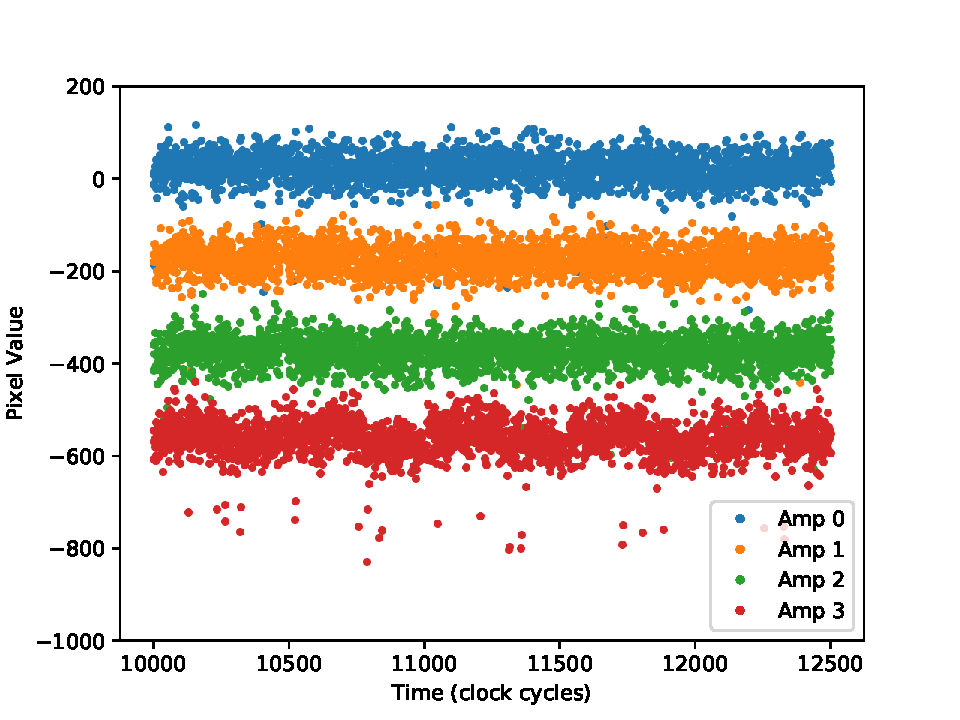
\includegraphics[width=.32\columnwidth]{pixeltime_series_1.pdf}
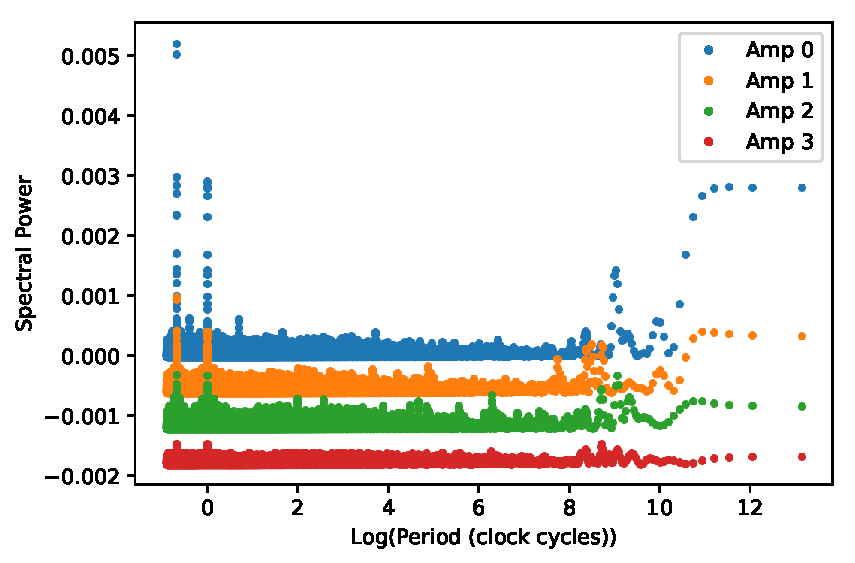
\includegraphics[width=.32\columnwidth]{all_amp_periodograms.pdf}
\caption{The time series for all 4 amplifiers share common-mode behaviors for some intervals but not always (left and middle plots).
This is visible in a short segment of the time series of all pixels for an example group up the ramp 53 in a dark ramp where the bias has already been subtracted.
The pixels time series smoothed with a 51 pixel-wide median filter to better see the low frequency noise.
The left panel shows the a time near the beginning of a frame, where amplifiers 1 ad 2 share some common-mode read noise.
The middle panel shows another part of the time series where Amplifiers 1 and 2 have more disparate noise signatures.
The right panel shows the periodogram of each amplifier's time series over the first 10$^5$ clock cycles (0.1) seconds, which exhibits no consistent peaks.
}\label{fig:darkPixelTimeSeries}
\end{figure*}


\subsubsection{PCA Correction}
Another approach to treating the 1/f noise is dimensionality reduction with Principal Component Analysis.
Here, we assume that the counts for each pixel along a column is a random variable that can be correlated with pixels in other columns.
Each row represents a different noise iteration.
First, we calculate the mean value of each pixel in the 108 group stack and subtract all groups by this mean image.
This removes all bias levels and focuses on the time variability of the pixels.
Here, we assume the dark current is negligible.
Next, we mask all bad pixels by setting all pixels with $| f | > 200$ DN to 0 DN to remove bad pixels that can drive the principal components.
The first 10 principal components are plotted in Figure \ref{fig:pcaEigenvectors} for two example groups (54 and 55).

The first 10 principal components explain 14\% of the total variance in each group up the ramp.
The principal components from one group to another are different, but the ordering of these components generally follows a pattern of increasing frequency with higher order principal components.
This is expected for 1/f noise where the lowest frequencies have most of the power.
Since the first principal components are different from one group to another, we calculated the principal components for each group independently.
We then create a noise model image which is the matrix multiplication of the eigenvectors by the principal components for 10 components.
This model is subtracted from each group to create a 1/f-corrected image.

The PCA subtraction is applied to each group up the ramp and then these groups are subtracted in pairs to create a time series.
We use 20 principal components as a starting point for this method.
The final time series has and measured standard deviation of 5,300 to 5,500 DN within the background-subtracted aperture.
This is comparable to the row and column subtraction standard deviation of 5,500 to 6,500 DN.
Adding 10 more principal components for a total of 20 eigenvectors only reduces the time series noise to 5,100 to 5,400 for the 3 apertures.

\begin{figure*}[!hbtp]
\centering
\includegraphics[width=.4\columnwidth]{pca_dark_amp_all_extra_bias_sub_grp_54.pdf}
\includegraphics[width=.4\columnwidth]{pca_dark_amp_all_extra_bias_sub_grp_55.pdf}
\caption{The first 10 principal component eigenvectors identified from group 54 (left) and group 55 (right).
The pre-amplifier reset values are seen in the first principal component, and change from one group (one read in RAPID) to another.
The principal components generally increase in frequency with principal component number.
In other words, the highest frequency principal components explain the least amount of the variance as would be expected for 1/f noise.
}\label{fig:pcaEigenvectors}
\end{figure*}

In another approach, we treat each amplifier separately so that the principal components are calculated independently.
This approach means that a noise signature in 3 amplifiers but not the fourth does not propagate to fourth amplifier when subtracting the PCA-based model.
This individual-amplifier essentially has four times the number of degrees of freedom, so we fit with only the first 5 principal components in each amplifier.
The resulting eigenvectors are shown in Figure \ref{fig:pcaEigenvectorsIndAmp}.

If we treat each amplifier separately, the PCA model is more effective in reducing 1/f noise.
We begin by keeping 5 principal components within each amplifier and subtracting these from each amplifier separately.
The resulting standard deviation of the time series is 2500 to 3820 DN.
This is improvement is beyond what is possible on a real source because the principal components include pixels over the source aperture.
To simulate a real photometry scenario, it is necessary to interpolate over the source aperture points as done in Section \ref{sec:smoothKernelSub} for the smoothing kernel.

\begin{figure*}[!hbtp]
\centering
\includegraphics[width=.4\columnwidth]{pca_dark_ind_amp_grp_54_extra_bias_sub.pdf}
\includegraphics[width=.4\columnwidth]{pca_dark_ind_amp_grp_55_extra_bias_sub.pdf}
\caption{The first 5 principal component eigenvectors identified from group 54 (left) and group 55 (right) where each amplifier has been analyzed independently.
The amplifier boundaries are demarcated by solid vertical lines.
}\label{fig:pcaEigenvectorsIndAmp}
\end{figure*}

\clearpage

\subsubsection{Grism Aperture}
The NIRCam grism time series are particularly susceptible to 1/f noise because the dispersion direction is parallel to the detector's fast-read direction.
This is visible in Figure \ref{fig:longDarkGrism} where the grism apertures (in red) are parallel to the 1/f noise correlations.
The background subtraction along the spatial direction (vertically) will efficiently remove pre-amplifier offsets from frame to frame and amplifier to amplifier.
However, there are no side reference pixels or background regions available on the middle two amplifiers.
Therefore, the 1/f noise will adversely impact broadband behaviors of the lightcurves.
Without reference pixel subtraction, the grism apertures have standard deviations of 153,000 DN.
Reference pixel subtraction drops this value to 45,000 DN and row-by-row subtraction drops it to 9,000 DN.
For a well depth of 60\%, there are $1.0 \times 10^8$ DN of source counts in an exposure, which amounts to a photon error of 7,400 DN assuming a gain of 1.84.
Therefore, 1/f noise can potentially dominate the error budget for broadband grism time series!
Expressed in ppm, the read noise after processing with row-by-row subtraction is 90 ppm as compared to a photon noise of 74 ppm for a CDS subtraction (2 groups in ramp).

The timescale of most interest to studying atmospheres is the transit duration when trying to assess the stability.
The transit durations for most exoplanets considered is several hours long.
We therefore quantify error source over 1 hour duration.
If the smallest stripe subarray is used, frame time is 0.34 seconds.
For simplicity, assuming a duty cycle of 80\% due to detector resets, there are 8460 frames over which to average read noise.
Therefore, the final read noise is only expected to be 1.4 ppm over a 1 hour timescale if each frame is statistically independent.
In section \ref{sec:darkBaseline}, we show from dark frames, that the read noise is statistically independent from integration to integration.

For a concrete example, we consider a primary transit of WASP-80 b observed with the F444W grism time series mode.
The exposure parameters that give a peak pixel count of 35,000 DN or 40\% well depth are a 2048$\times$256 stripe mode with BRIGHT1 read mode for 12 groups.
These integrations are 31 seconds in duration.
Each integration will have a 7.8$\times 10^7$ DN in a broadband aperture, so the photon noise per integration is 6,500 DN or 83 ppm.
Over 1 hour (111 integrations), the photon noise will be 8 ppm if all integrations are independent.

\begin{figure*}[!hbtp]
\centering
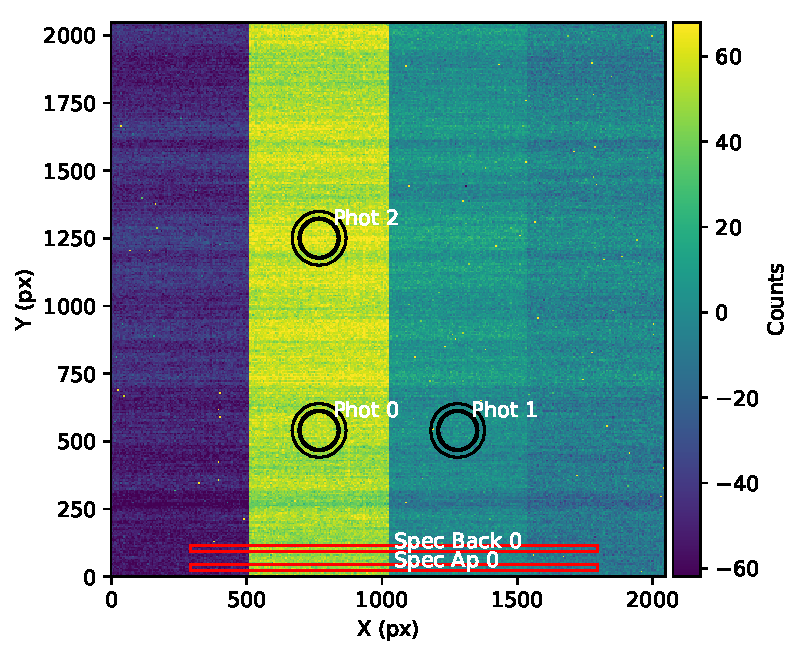
\includegraphics[width=.32\columnwidth]{aps_3_NRCNRCALONG-DARK-72350742131_1_485_SE_2017-08-23T16h49m51_int_015_014.pdf}
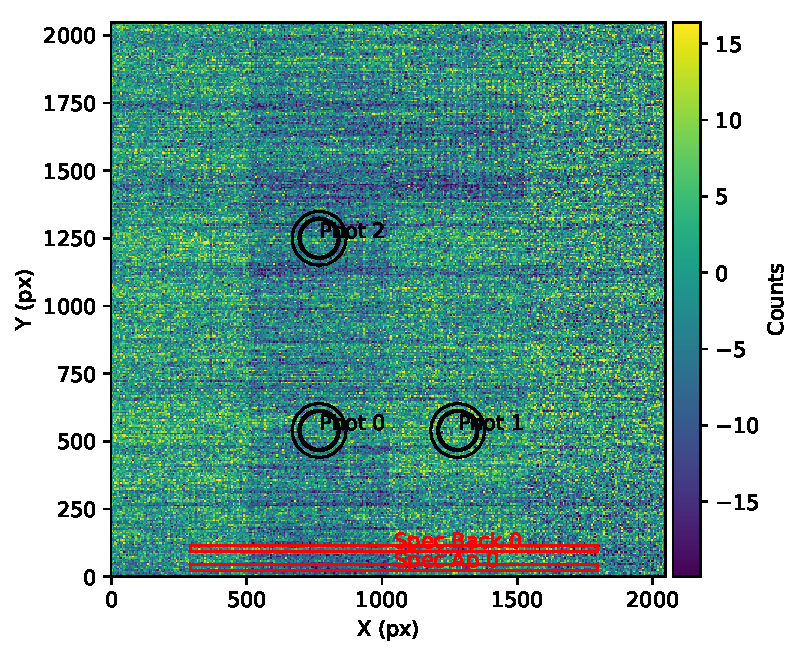
\includegraphics[width=.32\columnwidth]{aps_0_NRCNRCALONG-DARK-72350742131_1_485_SE_2017-08-23T16h49m51_red_int_015_014.pdf}
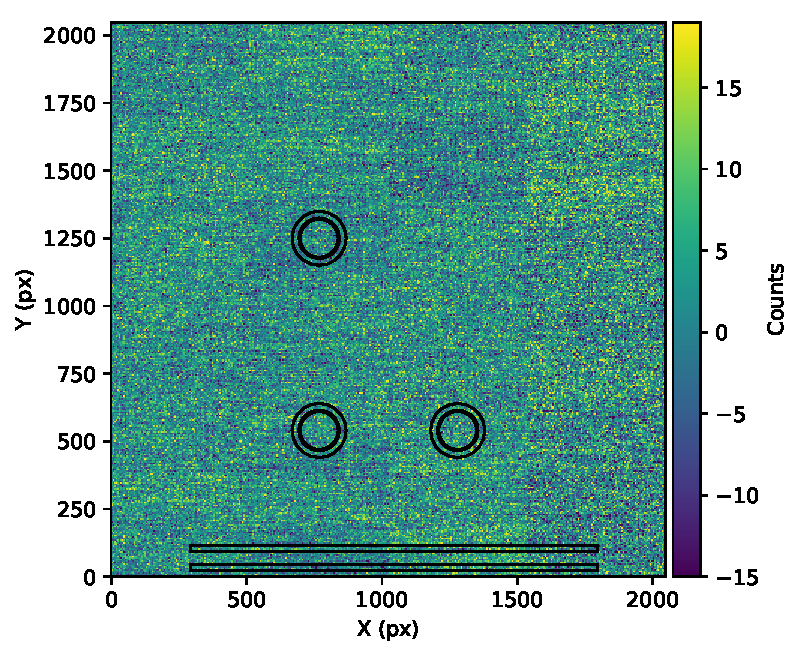
\includegraphics[width=.32\columnwidth]{aps_1_NRCNRCALONG-DARK-72350742131_1_485_SE_2017-08-23T16h49m51_red_int_015_014_rowColSub.pdf}
\includegraphics[width=.32\columnwidth]{long_dark_darkGrismApA5raw.pdf}
\includegraphics[width=.32\columnwidth]{long_dark_darkGrismApA5red.pdf}
\includegraphics[width=.32\columnwidth]{long_dark_darkGrismApA5redRowCol.pdf}
\caption{Time series of a grism photometric broadband aperture during a long dark exposure for detector ALONG=A5. As in \ref{fig:longDarkPhot}, the long dark exposure of 108 frames is used to construct 54 pairs of reads that are subtracted, in analogy with a series of integrations.
The photometric aperture is made to represent a similar one to the F322W2 grism trace.
}\label{fig:longDarkGrism}
\end{figure*}


%% See the notebooks wlp8_psf_image.ipynb and noise_sources_wlp8.ipynb for calculations
\subsubsection{The impact of correlated read noise on time series}
We consider here some example science impacts of correlated read noise in these photometric apertures.
We will evaluate the performance of a WEAK LENS +8 mode photometric time series, as will be common with NIRCam grism time series observations.
For a pessimistic scenario, we assume a 15,000 DN read noise contributes to every pair of reads for the 70 pixel radius aperture (and 75 to 100 pixel background subtraction annulus).
If the read noise is tolerable under this scenario, then it should have a minimal impact on photometric time series.
If it is a problem, we will discuss methods of mitigation such as the row-by-row subtraction above.

We also assume that each read/frame is statistically independent from the other.
Therefore, the uncorrected read noise per integration is:
\begin{equation}
RN_{ap,70,75,100} = \frac{21,200 DN}{ \sqrt{N_{frames}}} \approx \frac{46,000 e^-}{ \sqrt{N_{frames}}},
\end{equation}
where $N_{frames}$ is the number of frames in an integration and a gain of 2.17 $e^-$/DN is assumed for the A3 detector.
If there are 2 frames in an integration, we recover 15,000 DN for the case of a read pair subtraction on the A3 detector.
\textcolor{red}{\bf Make sure I scaled this correctly both for the read pair subtraction and a slope fit. Also empirically verify this with a slope fit to multiple images.}
For an integration that fills to a peak of $\sim$ 60\% well depth or 35,000 DN, the integrated DN counts for a WEAK LENS +8 PSF would be $1.8 \times10^8$ DN, having a photon uncertainty of 9,100 DN or 51 ppm.
Therefore, the correlated read noise, if left uncorrected, will have a highly significant ($>50\%$) impact on an integration of 5 or fewer frames that fill to 60\% well depth.
As an example, a $K$=8.5 magnitude star observed in full frame WEAK LENS +8 imaging mode with 6 RAPID groups up the ramp sampling and the F210M filter would have a photon noise equal to the (uncorrected) read noise and fill the detector to 54\% well depth.

We have demonstrated that row-by-row and amplifier-by-amplifier median subtraction can substantially reduce the read noise for a correlated double sample subtraction from 23,500 DN to 2,900 DN.
Therefore, the corrected read noise per integration should be:
\begin{equation}\label{bestRNCorrection}
RN_{ap,70,75,100} = \frac{4,100 DN}{ \sqrt{N_{frames}}}
\end{equation}
\textcolor{red}{\bf This is for the ALONG detector.
Update for the A3 detector}
For the same $K$=8.5 magnitude star observed in full frame imaging WEAK LENS +8 imaging mode, the read noise per integration should be 1,700 DN.
Fortunately, this is now a small fraction of the photon uncertainty of 9,100 DN and only amounts to an increase in noise over the 51 ppm photon by 9 ppm per integration.


\textcolor{red}{\bf Include more calculations on how the individual frame read noise would impact many frames in a time series of a bright target vs a faint target.}

\subsection{Goddard Cryogenic Vacuum (CV) Stability Tests}

During the Cyrogenic Vacuum Test 3, the Integrated Science Instrument Module (ISIM) was placed in a vacuum chamber with the Optical telescope element simulator (OSIM).
The ISIM has all the instruments with their internal optics and detectors but no telescope mirrors.
The OSIM simulates the PSF expected when a star or other point source illuminates the JWST instruments.
While other tests described in this work illuminated the science instrument detectors in different ways, the point spread function most closely resembled the JWST flight point spread function.

CV3 included a series of exposures over nearly 24 hours with an LED lamp in imaging mode to test the fundamental photometric performance.
The LED was a narrowband source at 1.55 $\mu$m, which was used in imaging mode since this would result in a narrow-lined spectrum.
While the spectroscopic modes are expected to be the most scientifically interesting modes for studying exoplanet atmospheres, the broadband lamps needed to produce a spectrum tend to be less stable than LEDs.
Therefore, the test was designed with an LED with the hope of measuring the precision possible with the NIRCam optics and detector.

As with the spatial scanning mode on HST \citep[e.g.][]{mccullough2012spatialScan,deming13}, spreading the light of a source over many pixels can improve the precision of spectroscopy.
This is also accomplished by ground-based observatories by either de-focusing the telescope \citep{southworth2009defocusing} or by employing a beam-shaping diffuser \citep{stefansson2017diffusers}.
By spreading the light source over many pixels, the light curve becomes less sensitive to flat fielding or intra-pixel sensitivity errors with telescope pointing jitter or seeing variations during an observation.
Similarly, NIRCam can employ a weak lens to defocus a star's light.
Figure \ref{fig:WLP8PSF} show the PSF of the +8 wave defocused images during the CV3 stability tests.
The hexagonal PSF is summed with circular aperture with a radius of 70 pixels.
The central peak may used to find a centroid of the star and center the circular aperture.

\begin{figure}[!hbtp]
\centering
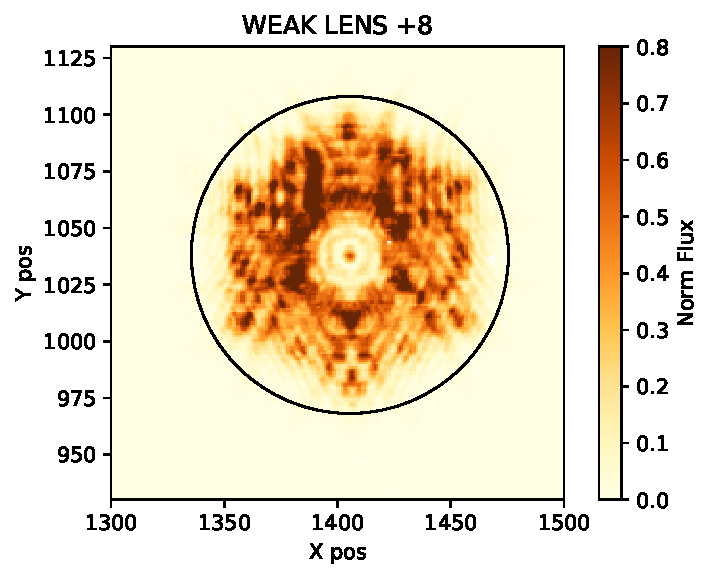
\includegraphics[width=.49\columnwidth]{wlp8_psf.pdf}
\caption{Weak Lens +8 PSF during CV3 testing.
The central peak is used for centroiding, while the entire PSF is used for aperture photometry.
A 70 pixel radius aperture (shown here is a black circle) is used for the source aperture.}\label{fig:WLP8PSF}
\end{figure}

A series of detector stability tests was performed using this +8 wave weak lens and 1.55 $\mu$m LED in a few different modes.
A time series of all possible modes is shown in Figure \ref{fig:CV3longTser}.
The full frame modes (FULL1 through FULLQ) used 2 samples of the ramp for integration times of 21.5 seconds whereas the subarrays were tuned to have a similar integration time (21.3 sec for 20 Groups of a 320$\times$320 subarray and 25.1 seconds for 6 groups of a 640$\times$640 subarray).
This ensured that during these 4 different types of subarray/full frame window sizes, the well depths achieved were similar.

It is apparent from Figure \ref{fig:CV3longTser} that the WLP8SUB test with a 320$\times$320 subarray and 20 groups of the ramp has smaller scatter than the FULL1 through FULLQ tests.
After removing a linear fit to the time series (to account for long term trends in the lamp), the standard deviation of the WLP8SUB data is 500 ppm whereas the FULL tests range from 1020 to 1540 ppm.
For the FULL 2048$\times$2048 pixel integrations with 2 groups up the ramp, the count rate of photons is calculated in each pixel by subtracting the two groups (ie two reads for this RAPID mode) from each other and dividing by the group time (time between these two reads for this RAPID mode).
For the WLP8SUB mode, a linear least squares fit is performed to the groups as a function of time and the slope of this line is the count rate on a pixel.
The large number of groups used to fit this line ensures that the read noise is reduced by $\sim 1/\sqrt{N_G}$, where $N_G$ is the number of groups.

There are two explanations for why the WLP8SUB mode shows less scatter than the FULL modes, 
\begin{enumerate}[noitemsep]
	\item The reduction of read noise improves the stability of the signal and\label{item:readNReasonCV3subFull}
	\item That the lamp is variable on short time scales of a frame (10.74 seconds).\label{item:lampReasonCV3subFull}
\end{enumerate}
The read noise of a pixel is $RN_1 \approx$ 15 e$^-$ for the short wavelength arrays\footnote{https://jwst-docs.stsci.edu/display/JTI/NIRCam+Detector+Performance} in this test.
If this is uncorrelated across the 70 pixel aperture source radius, the read noise from two groups  (correlated double sampling) on the total aperture is $RN_{tot} = \sqrt{N_{s,px}} RN_{CDS} = \sqrt{\pi} r_{s,px} RN_{CDS}$ = 124 * 15 e$^-$ = 1861 e$^- \approx 930 $DN.
This amounts to 25 ppm, which is a small compared to the photon noise (113 ppm).
Furthermore, the read noise for 20 groups is $RN_{20} \approx 6e^-$ would ammount to a 10 ppm, so a difference from the CDS readout of only 15 ppm. {\textbf{\textcolor{red}{(Note, here I have used the effective read noise for 90 groups on JDox, but should corrected to 20 groups)}}}
This is dramatically smaller than the observed difference in standard deviation (500 ppm in subarray with 20 groups and 1020-1540 ppm in full frame in 2 groups).
However, if there are correlated components to the read noise in this large aperture, the read noise could be higher.

Under scenario \ref{item:lampReasonCV3subFull}, the short timescale variations of efficiently averaged out by sampling the reads multiple times up the ramp.

\begin{figure}[!hbtp]
\centering
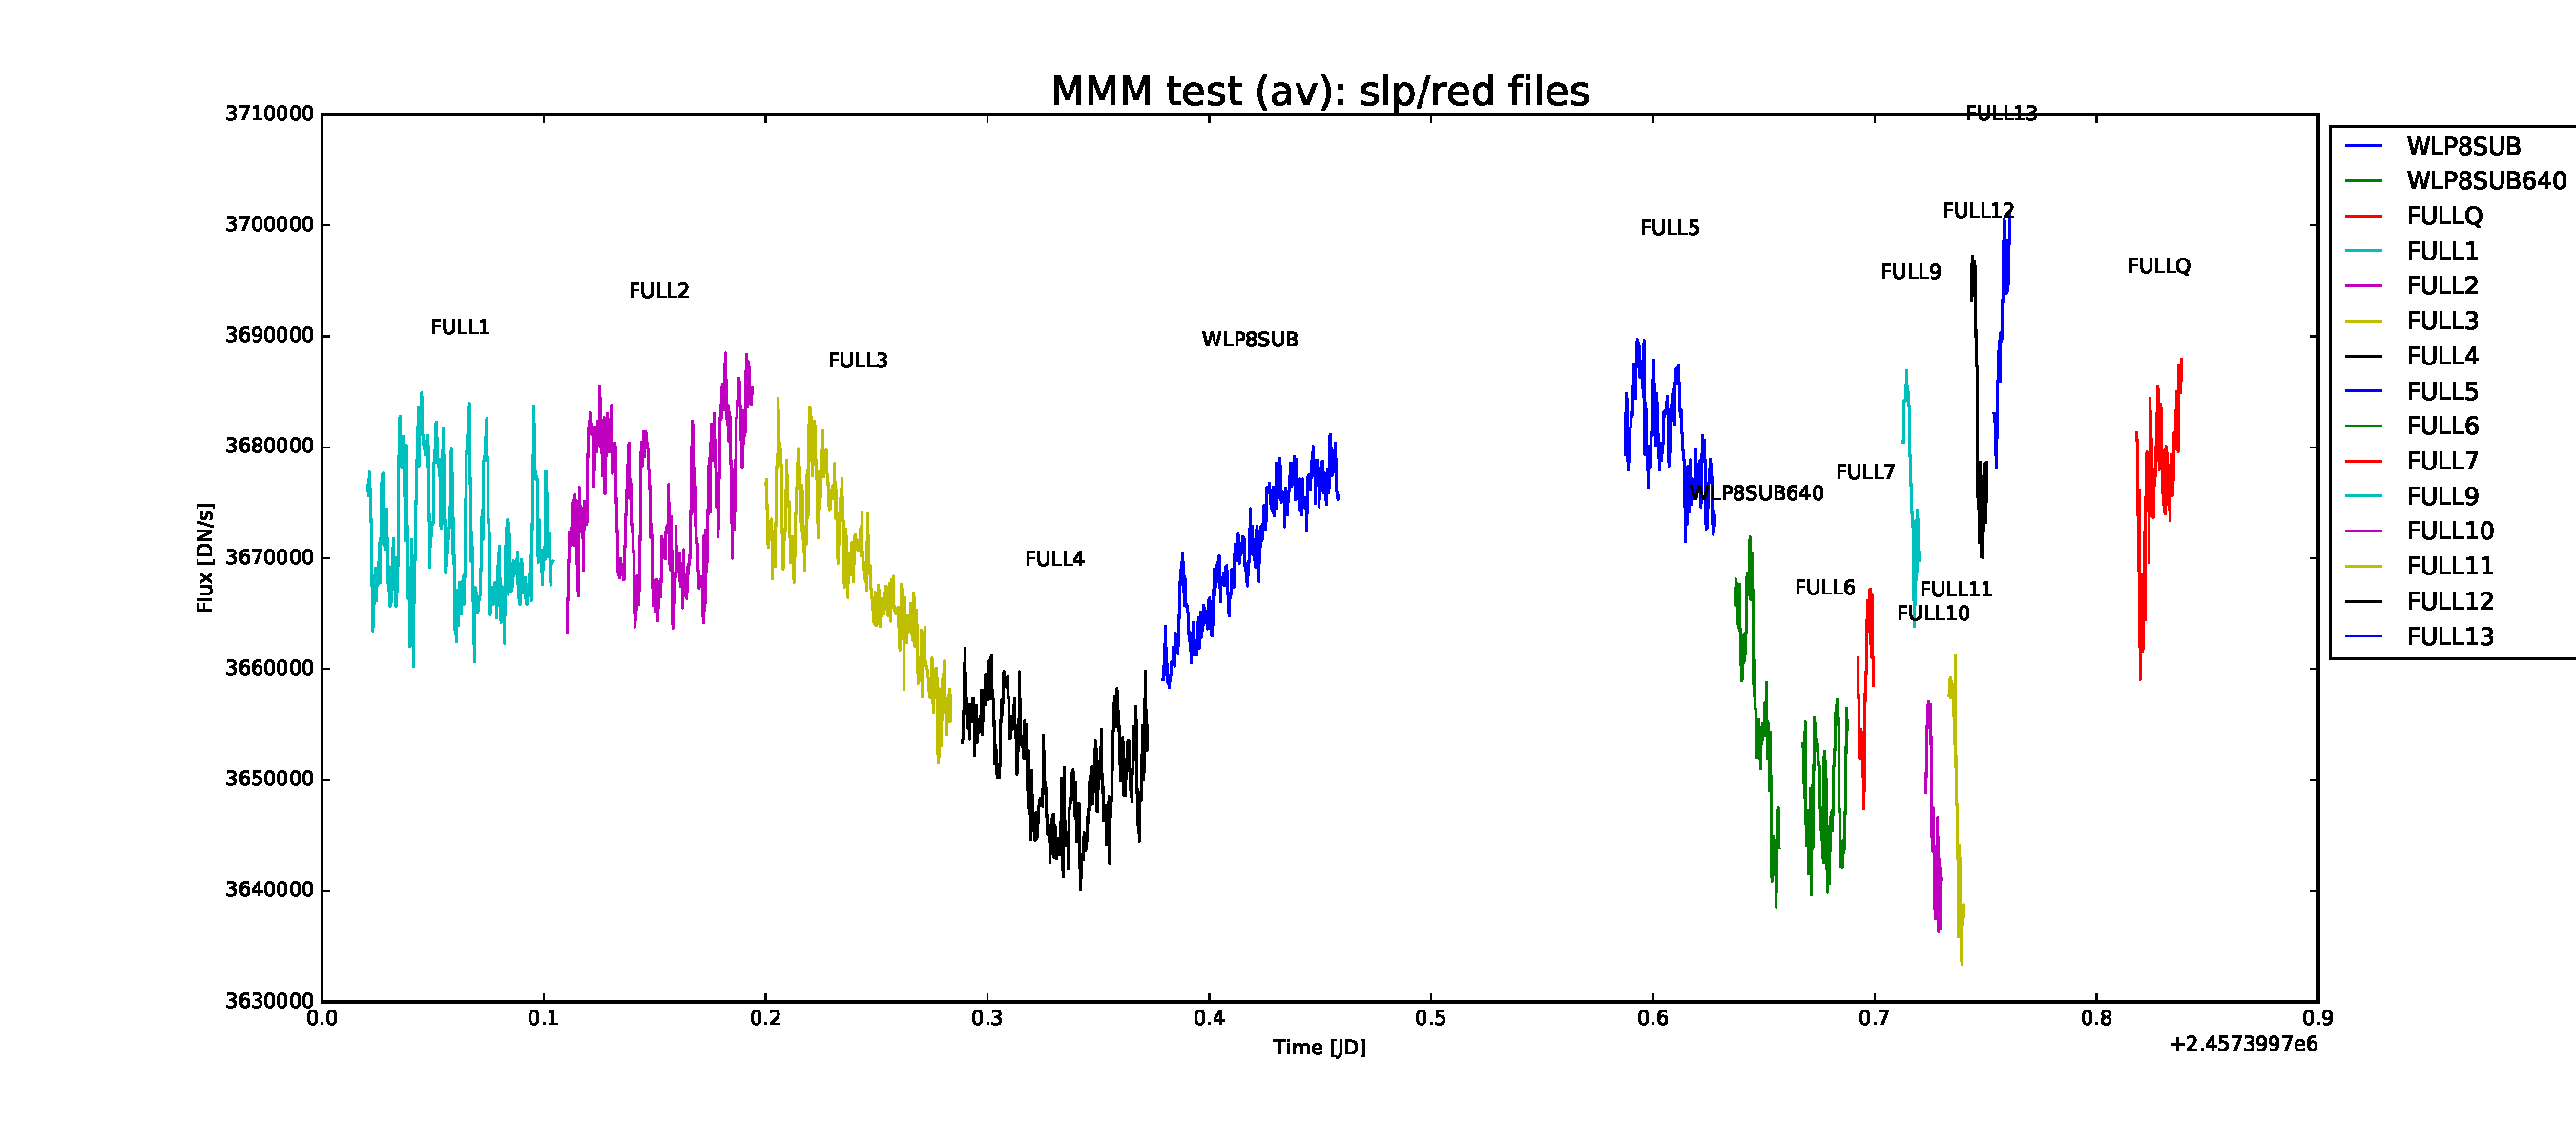
\includegraphics[width=.79\columnwidth]{plot_mmm.pdf}
\caption{Time Series plot through the CV3 photometric stability campaign.
All test shown above were using the Weak Lens +8 mode, with a PSF as shown in Figure \ref{fig:WLP8PSF}.
13 tests (FULL1 through FULL6) are all in full frame mode, while SUB used a 320$\times$320 subarray and SUB640 used a 640$\times$640 subarray.
The WLP8SUB showed smaller standard deviation that the full frame tests, when the linear trend is removed.}\label{fig:CV3longTser}
\end{figure}

\subsection{Lessons Learned from CV3 Tests}\label{sec:CV3Lessons}
Although the light curves from the CV3 stability tests were not able to achieve photon-limited performance to study the precision of transit and eclipse spectroscopy, there were some lessons learned from this data.
We were able to determine the best practices for the pipeline and analysis by running the raw data through the pipeline and changing the steps to produce light curve.
We experimented with the methodology for turning raw detector reads up the ramp into count rates on the detector, the intrapixel capacitance (IPC) correction, flat fielding, reference pixel correction and detector non-linearity.
After the calibrated images are created, we experimented with different types of aperture photometry including different geometries, background calculations and aperture sizes.

After experimenting with these configurations, we find the following pipeline steps are important:
\begin{itemize}
	\item Fitting a line up the ramp gives superior results to subtracting the last and first pairs of read (as expected by reducing the read and electronic 1/f noise)
	\item Centering the aperture with the central spot inside the hexagon is important to conserve the flux within the aperture
	\item Row-by-row subtraction (along the detector's fast-read direction) gives superior background subtraction to traditional aperture photometry (using the mean or robust average value in a background annulus)
	\item Aperture sizes for the source at ~70 pixels, outside the hexagon, gave the best precisions
	\item An annulus aperture on the source (including the inner and outer edges of the hexagonal PSF) usually gives the best precision light curves
\end{itemize}

We also found reduction steps that had very little impact on the final photometric precision including
\begin{itemize}
	\item IPC corrections ($\lesssim 0.01$ ppm)
	\item Flat-fielding ($\lesssim 0.3$ ppm)
\end{itemize}
We summarize the lessons from the tests here.

\clearpage
\subsection{OTIS Tests}

A series of NIRCam stability tests were carried out while the entire JWST telescope system was placed in a tall vacuum chamber at NASA Johnson.
However, there is no feasible way to place a point source lamp at infinity to simulate the imaging of astrophysical objects onto a JWST instrument, so an alternate lamp setup is used.
During these tests, there were two configurations 1) the ``half pass" tests where lamp sources within the optical system and 2) ``pass and a half" tests where the a lamp source within the optical system bounces light off the secondary, primary, flat mirrors mounted on the chamber's ceiling and then through the entire telescope and instrument chain to the detectors.

\subsubsection{Pass and a Half Grism Time Series Test - Photometry}
The OTIS testing included a time series mode similar to the grism time series template used in orbit for transiting planets.
Figure \ref{fig:otisPSFs} shows the point spread functions for the OTIS tests that simultaneously illuminated the short wavelength and long wavelength channels.
The ``O9'' supercontinuum illuminated the detector over a wide wavelength range from 2.5 to 4.1$\mu$m.
A small fraction of the light is emitted at wavelengths shorter than 2.5 $\mu$m, which is sufficient to illuminate the short wavelength detector to peak counts of $\sim 260$DN per exposure.
Meanwhile, the peak of the grism is $\sim$ 26,000 DN.
This lamp configuration was a pass and a half test, which suffered from the vibrations and oscillations of the suspension system, which can be perturbed by motors such as vacuum pumps.
The telescope is suspended vertically and can potentially swing under these vibrations.

The point spread function through the weak lens and optical setup create a very unusual point spread function for the short wavelength channel, shown in Figure \ref{fig:otisPSFs} that has multiple clumps of emission.
We perform aperture photometry on a knot of emission at (1090 px, 230 px) for the short wavelength detector.
This knot is concentrated enough to fit with a 2D Gaussian and centroid this Gaussian to ~0.2 pixels, which can be used to track the motions of the PSF due to the position oscillations.
For the long wavelength detector, we initially extract a box aperture to create a broadband light curve.


\begin{figure*}
\gridline{\fig{wlp8_otis_psf.pdf}{0.7\textwidth}{WLP8 Image} }
\gridline{\fig{{grism_otis_psf.pdf}}{0.7\textwidth}{Grism Image}}
\caption{Median images of the short wavelength (SW) weak lens mode and long wavelength (LW) grism spectroscopy that were used simultaneously in a grism time series stability test.
Due to the OTIS optics setup, the short wavelength WLP8 image does not nearly represent the hexagonal PSF from CV3 (Figure \ref{fig:WLP8PSF}) or flight.
We perform photometry on a single knot of emission as highlighted as the blue circular aperture.
For the grism time series broadband test, we use a rectangular aperture and a vertically offset background box.
}\label{fig:otisPSFs}
\end{figure*}

\begin{figure*}
%\gridline{\fig{tser_LW_OTIS.pdf}{0.99\textwidth}{WLP8 Image} }
\gridline{\fig{tser_LWSW_OTIS.pdf}{0.6\textwidth}{Grism Time Series}}
\caption{Time series of the simultaneous SW/LW Time Series Stability test.
The image motion in this test due to vibrations and oscillations is two orders of magnitude larger than expeced in flight.
The complicated PSF and low signal on the short wavelength channel compromise its sensitivity whereas the long wavelength broadband flux is dominated by lamp instability.
}\label{fig:otisLWSWtser}
\end{figure*}


The locations of the subarrays have ROWCORNER=431.
This means there are not top or bottom reference pixels.
If we use a horizontally-displaced background region, the pre-amp offsets will not be properly subtracted.
We therefore subtract the median from each column and then each row (not including the grism aperture).
We subtract the median of each column first to remove the amplifier offsets and then the median of each row second to reduce the 1/f noise.
Figure \ref{fig:otisLWcolrowSub} shows the dramatic effect of subtracting the columns and rows from each aperture.

\begin{figure*}
%\gridline{\fig{tser_LW_OTIS.pdf}{0.99\textwidth}{WLP8 Image} }
\gridline{\fig{raw_tser_LWgrisMPPVertBackbox_otisSWLWsimult.pdf}{0.49\textwidth}{Slope Images}
\fig{raw_tser_LWgrisMMMRowColSubVertBackbox_otisSWLWsimult.pdf}{0.49\textwidth}{Column-by-column and row-by-row subtraction}}
\caption{The grism time series contains correlated read noise due to pre-amplifier offsets over each amplifier and 1/f noise in the horizontal (fast read) direction.
Row-by-row-subtraction dramatically decreases the noise due to 1/f noise while column-by-column subtraction dramatically decreases the pre-amplifier offset noise.
}\label{fig:otisLWcolrowSub}
\end{figure*}

\subsubsection{Pass and a Half Grism Time Series Test - Spectroscopy}

\begin{figure*}
\gridline{\fig{comparison_spec_otis_flat_vs_no_flat.pdf}{0.55\textwidth}{}}
\caption{Flat fielding has a pronounced effect of reducing the crosshatch pattern in the spectrum.
There are small offsets in the flux os the spectrum also because of the flat field.
}\label{fig:otisLWflatVsNoFlat}
\end{figure*}


\begin{figure*}
%\gridline{\fig{tser_LW_OTIS.pdf}{0.99\textwidth}{WLP8 Image} }
\gridline{\fig{o9LEDwf322w2Flat_dyn_spec_NRCN83-256-O9LW}{0.49\textwidth}{Dynamic Spectrum}
\fig{o9LEDwf322w2Flat_dyn_spec_NRCN83-256-O9LW_aligned}{0.49\textwidth}{Dynamic Spectrum with Alignment}}
\caption{The dynamic spectrum of the grism along shows large artifacts due to motion of the source (broad horizontal stripes).
These are dramatically reduced when using cross correlation
}\label{fig:otisLWdynSpec}
\end{figure*}

%\begin{figure*}
%\fig{o9LEDwFlat_bb_series_NRCN83-256-O9LW.pdf}{0.41\textwidth}{Broadband Time Series}
%\end{figure*}

We also analyze the spectroscopic time series for the OTIS grism time series.
The extracted spectrum and dynamic spectrum (how each wavelength varies in time) can be seen in Figure \ref{fig:otisLWdynSpec}.
Flat fielding is important for removing the imprint of the crosshatch pattern, as visible in Figure \ref{fig:otisLWflatVsNoFlat}.

The wavelength-binned time series shows dramatic variations (shown in Figure \ref{fig:otisWavebinTSeries}) due to the shifts in the dispersion direction.

\begin{figure*}
\gridline{\fig{wavebin_tser_o9LEDwFlat_NRCN83-256-O9LW.pdf}{0.49\textwidth}{Time Series without Alignment}
\fig{wavebin_tser_o9LEDwf322w2Flat_NRCN83-256-O9LW_aligned.pdf}{0.49\textwidth}{Time Series with Alignment}}
\caption{The position variations along the dispersion direction cause large fluctuations in the time series.
These are dramatically reduced when cross-correlating and finding the peak to adjust for wavelength shifts
}\label{fig:otisWavebinTSeries}
\end{figure*}

\clearpage
\subsection{Using SW centroid for LW grism}

We attempt to use the centroids form the SW imaging as input for a broadband grism aperture.
This potentially provides a way to input centroid information without cross-correlating a spectrum.
However, the SW centroids add more noise to the photometry as seen in Figure \ref{fig:otisLWSWtserShift}.
\textcolor{red}{\bf Did I properly multiply shifts by -0.5?}

\begin{figure*}
%\gridline{\fig{tser_LW_OTIS.pdf}{0.99\textwidth}{WLP8 Image} }
\gridline{\fig{tser_LWSW_OTIS_w_shift.pdf}{0.6\textwidth}{Grism Time Series}}
\caption{Same as Figure \ref{fig:otisLWSWtser} but where the SW shifts were applied (with a scaling factor of 0.5) to the long wave.
The aperture shifting appears to increase the flux errors with centroid shifts.
}\label{fig:otisLWSWtserShift}
\end{figure*}


\subsection{Differential Spectrum}
We investigate whether the lamp fluctuations can be removed by dividing by a signal-to-noise-weighted broadband time series.
\begin{figure*}
\gridline{\fig{wavebin_tser_o9LEDwf322w2Flat_NRCN83-256-O9LW_differential.pdf}{0.49\textwidth}{Differential Time series}}
\caption{Differential time series
}\label{fig:otisLWDiffdynSpec}
\end{figure*}

\clearpage

\subsubsection{Half Pass Subarray Size Tests}

As with the CV3 tests in Section \ref{sec:CV3Lessons} and Figure \ref{fig:CV3longTser}, we found the highest precision lightcurves when using subarray read configurations.
Figure \ref{fig:OTISsubarrays} shows the many subarrays explored in a set of time series.
As the number of reads up the ramp becomes larger and larger, the standard deviation increases.
This would be expected if the read noise contributed significantly to the standard deviation so that ramp fitting decreases the read noise.
The perplexing thing is, though, that this is even true if we throw away all the intermediate reads.
That is, with all readout modes, count rate (ie. slope image is approximated by the last subtracted by the first read.
Here the number of reads in between these is irrelevant.
A possible way to explain the superior standard deviation for the smallest 2048$\times$64 subarray is not that more reads increase precision on the slopes but rather the small subarray has a smaller contribution from spatially correlated noise.
When larger frames are read out, for example, the 1/f noise becomes increasingly uncorrelated from read to read.\textcolor{red}{Wrote this when very tired. Is this correct and logical?}

Note that the integration times are different for these 4 tests. They are 39.9, 39.9, 32.3, 31.8 and 32.2 for the 64-STRIPE, 128-STRIPE, 256-STRIPE, 256-WIND and FULLFRAME respectively. Perhaps the lamp has oscillations on a timescale that are averaged out efficiently at 39.9 seconds but not 32.3 seconds?

\begin{figure}[!hbtp]
\centering
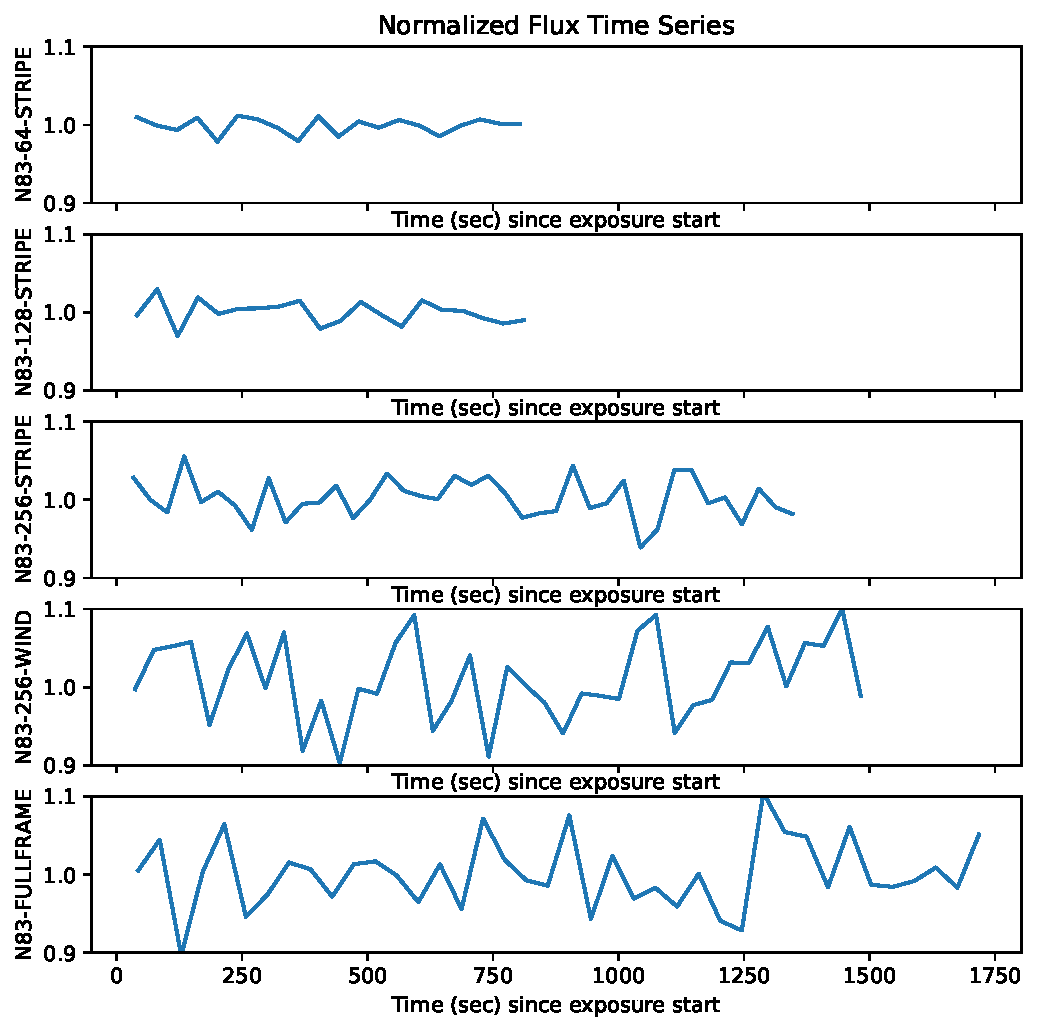
\includegraphics[width=.5\columnwidth]{subarray_config_tser.pdf}
\caption{A variety of subarrays in the OTIS stability tests were read out with similar integration times (32 to 39 seconds) to compare relative precision of the read modes. 
The time series are ordered vertically in increasing frame duration (and decreasing number of groups up the ramp) toward the bottom.
With this very crude box extraction (and no background subtraction), the standard deviation decreases as the number of groups up the ramp becomes more numerous.
This is likely related to correlated 1/f noise in the horizontal direction that is averaged out by more reads up the ramp.}\label{fig:OTISsubarrays}
\end{figure}

\begin{figure}[!hbtp]
\centering
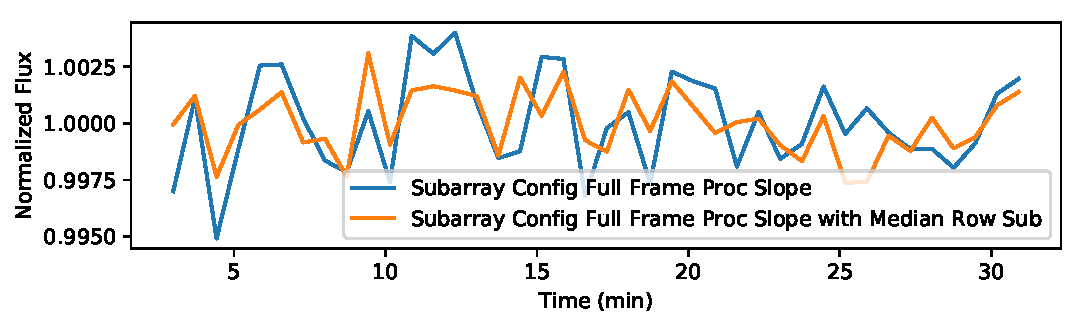
\includegraphics[width=.5\columnwidth]{fullframe_background_sub_compare_tser_tools.pdf}
\caption{An experiment with circular background-subtracted photometry shows dramatically improved precisions over raw aperture sums in Figure \ref{fig:OTISsubarrays}.
Additionally, a median subtraction of all background pixels per row improves the precision.}\label{fig:OTISSubConfigCircularAp}
\end{figure}

\begin{figure}[!hbtp]
\centering
\includegraphics[width=0.48\columnwidth]{apertures_for_NRCN83-128-STRIPE-72.pdf}
\includegraphics[width=0.48\columnwidth]{apertures_for_NRCN83-256-STRIPE-72.pdf}
\includegraphics[width=.48\columnwidth]{subarray_config_tser_backsub_rect.pdf}
\caption{Subarray configuration test during OTIS. The position of the background subtraction box has a dramatic effect on the precision of the time series.
This is due to correlated 1/f noise along the horizontal fast-read direction.
If the background subtraction box is on an adjacent amplifier, it captures a very different 1/f noise behavior than if it is on a shared amplifier.
The amplifier boundary is shown as a vertical blue dashed line.
\textcolor{red}{To do: understand better why the vertically offset box is better? Also, show the aperture as a separate figure.}
\textcolor{blue}{Now I understand it as coming from which amplifier the background box is on.}}\label{fig:OTISRectBacksub}
\end{figure}

\clearpage
\subsection{GL Dewar Tests}
\begin{figure*}
\gridline{\fig{ap_labels_S02illum_GLrun104.pdf}{0.32\textwidth}{Apertures}
		\fig{raw_tser_phot_S02illum1miAll_GLrun104.pdf}{0.32\textwidth}{Raw time series}
		\fig{refcor_phot_S02illum1miAll_GLrun104.pdf}{0.32\textwidth}{Ratio Time Series}}
\caption{Two photometric apertures are placed on the subarray, where they both see common-mode variations in the lamp.
The ratio of the time series of each aperture shows a handful of integrations at the beginning that stand out, which quickly stabilize to the 240 ppm level.
}\label{fig:GLtSeries}
\end{figure*}

The GL dewar, located at the University of Arizona, is a laboratory setup for assessing NIRCam flight and spare detectors.
The key difference with the Asic dewar discussed below is that the detector readout electronics are completely different, using a Leach system that is operated outside of the dewar as opposed to the Asic, which is lives right next to the detectors at cryogenic temperatures.
Comparing the GL dewar results to the asic dewar can be helpful in isolating the source of noise sources in the NIRCam system.
If the GL dewar and asic dewar share the same types of correlated noise sources, these can be attributed to the detectors.
If the asic dewar introduces or eliminates some correlated noise sources, these can be attributed to the readout electronics.

For the GL dewar, an LED illumination source flood-illuminates the detectors and the arrays are read out in subarray mode to create time series.
Figure \ref{fig:GLtSeries} shows the detector subarray illumination as well as two apertures that were used for time series photometry.
The first handful of frames show an initial ``warmup" period lasting about 9 seconds.
This quickly stabilizes to a 1200 ppm standard deviation likely dominated by lamp variations.
If one divides the two apertures by each other, the resulting time series is very flat and stable to within 260 ppm.
As with the Asic dewar, we find very good performance when comparing two apertures within the same detector.
This can be the result of common-mode systematic errors that divide out, so it is also important to check the time series against an independent detector.

\begin{figure*}
\gridline{\fig{ap_labels_S02illum1miAllBacksub_GLrun104.pdf}{0.32\textwidth}{Apertures}
		\fig{raw_tser_phot_S02illum1miAllBacksub_GLrun104.pdf}{0.32\textwidth}{Raw time series}
		\fig{refcor_phot_S02illum1miAllBacksub_GLrun104.pdf}{0.32\textwidth}{Ratio Time Series}}
\caption{We repeat the time series as Figure \ref{fig:GLtSeries} but add a vertically displaced background subtraction box to each aperture.
The background boxes reduce the ``ramp-up'' effect and longer timescale variations of the detector.
The ratio of the time series of each aperture has a larger scatter larger than Figure \ref{fig:GLtSeries} because subtracting the background adds to the 1/f noise (correlated along the horizontal direction) rather than reducing the 1/f noise.
}\label{fig:GLtSeriesBacksub}
\end{figure*}

We also introduce a background aperture, shown in Figure \ref{fig:GLtSeriesBacksub} to remove background variations and any amplifier offsets that could affect the flux.
The resulting time series has a smaller amplitude ``warmup'' and smaller oscillations than Figure \ref{fig:GLtSeries}.
When we divide the background-subtracted flux for each aperture by the other to make a ratio time series, the resulting noise is higher than in Figure \ref{fig:GLtSeries}.
This indicates that the background subtraction step introduces more noise than it removes when comparing the differential flux between the two apertures.
We suspect that 1/f noise in the background aperture causes this increase.
To conclude, background subtraction improves the absolute flux stability but worsens the differential flux across the apertures.
When observing an exoplanet time series, for example, scientists may wish to use one reduction technique for the absolute time series to derive the planet orbital parameters, say.
Then, when analyzing the spectrum, they may wish to use an alternate technique to assess the differential flux from one wavelength to another.

\subsubsection{Across Detectors}
We also examine the time series across detectors from ``Run104'' to test whether there are systematics unique to each detector/readout electronics.
We compare aperture photometry on the S02 versus S03 detector with background subtraction.
The resulting time series are shown in Figure \ref{fig:GLtSeriesAcrossDetectors}.
We an Allan variance diagram to show how well the flux scales like $\sqrt{N}$ statistics for $N$ integrations.
The curves track the expected $\sqrt{N}$ behavior but lie well above the theoretical read and photon noise limit.
This is likely because the 1/f noise is highly correlated within the aperture whereas the theoretical and photon noise limit assumes that the noise in each pixel is independent.
We do not quire reach the noise levels interesting to the exoplanet noise regime (30-100 ppm).

\begin{figure*}
\gridline{\fig{raw_tser_crossDetectorS02Backsub_GLrun104.pdf}{0.48\textwidth}{Time series for S02 detector}
		\fig{raw_tser_crossDetectorS03Backsub_GLrun104.pdf}{0.48\textwidth}{Time series for S03 detector}}
		\fig{allan_var_removelinear_True_gl_across_detectors.pdf}{0.48\textwidth}{Allan variance diagram for the ratio of the S02 to S03 background-subtracted detector fluxes}
\caption{Time series for background-subtracted rectangular photometry on the S02 and S03 detectors.
The ratio of the two detectors' fluxes, after background subtraction, scales like $\sqrt{N}$ statistics down to the 200 ppm level, but how it works below the 100 ppm is not measurable with this test.}\label{fig:GLtSeriesAcrossDetectors}
\end{figure*}

\begin{figure*}
\gridline{\fig{all_var_gl_dewar_run112_sub4_hi4_side_backsub_removelinear_True_3.pdf}{0.48\textwidth}{Allan Variance}}
\caption{The same test as Figure \ref{fig:GLtSeriesAcrossDetectors} shows {\bf dramatically} smaller noise if (1) the aperture size is increased and (2) a horizontally displaced aperture is used to reduce 1/f noise.}\label{fig:GLtSeriesRun112}
\end{figure*}

\clearpage

\subsection{Run 112 - Subarray 4}
We also investigate a slightly longer time series for GL dewar which approaches the timescales of interest to exoplanet transit lightcurves.
Figure \ref{fig:GLtSeriesRun112} shows the flux ratio between detectors S01 and S02 for the Run 112 Subarray 4 ``Hi4'' test.
The Allan variance plot again scales like the $\sqrt{N}$ statistics but above the theoretical noise limit.

\begin{figure*}
\gridline{\fig{azlab_ratio_tser_gldewar_run112_sub4_hi4_no_backsub.pdf}{0.48\textwidth}{Time series for S01 / S02 Ratio No Background Sub}
\fig{azlab_ratio_tser_gldewar_run112_sub4_hi4.pdf}{0.48\textwidth}{Time series for S01 / S02 Ratio With Background Sub}}
\caption{Time series for rectangular photometry on the S01 and S02 detectors as well as background-subtracted Rectangular photometry}\label{fig:GLtSeriesRun112}
\end{figure*}

\begin{figure*}
\gridline{\fig{all_var_gl_dewar_run112_sub4_hi4_no_backsub_removelinear_False_2.pdf}{0.48\textwidth}{Allan variance diagram no background subtraction}
\fig{all_var_gl_dewar_run112_sub4_hi4_with_backsub_removelinear_False_2.pdf}{0.48\textwidth}{Allan variance diagram with background subtraction}}
\caption{Allans variance for background-subtracted rectangular photometry on the S02 and S03 detectors.
The ratio of the two detectors' fluxes, after background subtraction, scales like $\sqrt{N}$ statistics down to the 200 ppm level, but how it works on longer timescales is not yet known.}\label{fig:GLAllanVarianceAcrossDetectors}
\end{figure*}

\subsection{Run 112 - Subarray 6}
Subarray 6 had higher lamp current and thus higher counts and lower photon noise, which approaches the exoplanet atmospheric feature regime (30-100 ppm).
In this test, we take the ratio of flux on one detector to the other.
This removes the lamp variations but allows the 


It was also important to take the ratio of S01 to S03, because this pair of detectors track each other much better than the S01 /S02.
This is surprising given that S01 is a short wavelength cutoff detector, S02 is a short wavelength cutoff detector and SO3 is a long wavelength cutoff detector.
Furthermore, the S01 and S02 detectors are powered by a different pair of cards than the S03 detector.


\begin{figure*}
\gridline{\fig{azlab_ratio_tser_gldewar_run112_sub6_hi4_no_backsub_biggerAp.pdf}{0.48\textwidth}{Time series for S01 / S03 Ratio No Background Sub}
\fig{azlab_ratio_tser_gldewar_run112_sub6_hi4_side_backsub_biggerAp.pdf}{0.48\textwidth}{Time series for S01 / S03 Ratio With {\it Side} Background Sub}}
\caption{Time series for rectangular photometry on the S01 and S03 detectors as well as side background-subtracted Rectangular photometry.
The background aperture was placed on the side reference pixels to reduce 1/f noise.}\label{fig:GLtSeriesRun112sub6}
\end{figure*}

\begin{figure*}
\gridline{\fig{all_var_azlab06_sub320_multi_exp_baseline_487_489_removelinear_True_489.pdf}{0.48\textwidth}{Allan variance for AZLab06 Long 320 Multi-Exposure Baseline}
\fig{all_var_gl_dewar_run112_sub6_hi4_side_backsub_removelinear_True_3_det_1_3.pdf}{0.48\textwidth}{Allan variance diagram for GL Dewar Run 112 Sub 6}}
\caption{Allan variance for background-subtracted rectangular photometry on the Asic Dewar versus the GL dewar.
Both tests use $320 \times 320$ subarrays, horizontally-displaced background apertures to remove 1/f noise and divide the two best-matched detectors.
For the GL dewar, the ratio of the two detectors' fluxes (after background subtraction) scales like $\sqrt{N}$ statistics down to the $\sim$60 ppm level where it begins to peel away from the $\sqrt{N}$ curve (green line).}\label{fig:GLAllanVarianceAcrossDetectorsSub6}
\end{figure*}

\clearpage
\subsection{Asic Dewar Tests}
We performed a variety of stability tests using a dewar with the same type of detectors, readout electronics and temperature control as the in-flight parts.
The detectors and asic controllers are devices that did not fully meet the flight requirements for NIRCam, but in many cases are close or above requirements.
The detectors are illuminated by short wavelength LEDs (1.6 to 1.8~$\mu$m) or long wavelength (3.0 to 3.6~$\mu$m) LEDs.
The LEDS are type LMS17LED-R and LMS34LED-R from Electro Optical Components, Inc.

The dewar has limited space for optical illumination so the LEDs' light is bounced off a convex mirror and painted aluminum surface before reaching the detectors.
The convex mirror, its support structure and a black mask at the edges of the detectors all produce a shadows on some pixels of the detector.
The illuminated portions of the detector are used for aperture extractions while the shadows are used for background subtraction apertures.

No LEDs used in ground-based tests were as stable as the desired precisions relevant to exoplanet targets (sub 30 ppm), so multiple arrays are used to correct for lamp variations during illuminated stability tests.
The best absolute stability of an LED measured on a detector was 0.05\% ppm over 2 hours.
More typically, the variations were 1\%, although the current measured with a multimeter was stable to 0.1\%.
A ratio time series is constructed by dividing the time series derived from one detector to another time series from a different detector.

\subsubsection{Persistence}\label{sec:persistence}
HST shows noticeable ramps with each HST orbit due to detector charge trapping \citep{zhou2017chargeTrap}.
Lamp sources in our laboratory tests typically have a warm up period lasting several tens of minutes, which makes it difficult to observe this same effect the detector ramps.
However, the charge trap release time is expected to the same when illuminated as compared to when turning the lamp off.
We therefore show a time series of an LED after it is turned off in Figure \ref{fig:persistence}.
In this experiment, the long wavelength detector is illuminated for 3 hours with fluence levels of about 300 DN/s.
At this fluence level and integration times of 9.4 seconds, each pixel reaches about 3000 DN in an integration.
Thus, the pixels are safely under saturation but have had plenty of time for the traps to reach equilibrium.

The characteristic timescale for persistence is 12 seconds, as shown in Figure \ref{fig:persistence}.
Thus, charge trapping release becomes undetectable after 5 minutes and is well below 0.1 DN/s per pixel.
This release time is considerably faster than for Hubble Space Telescope, where the fast-trap release timescale is 280 seconds and the slow-release timescale is 16,300 \citep{zhou2017chargeTrap}.


\begin{figure*}
{\gridline{\fig{ap_labels_B4persistence_AZLabStab01refcor.pdf}{0.5\textwidth}{Box Apertures}}}
{\gridline{\fig{phot_B4persistence_AZLabStab01refcor_tser.pdf}{0.5\textwidth}{Persistence Time Series}}}
\caption{The detector persistence timescale decays rapidly after the LED is turned off (vertical red line in bottom figure).
The source and background apertures are shown in the top image while the time series of counts per pixel are shown in the bottom figure.
The characteristic timescale for charge trapping is 12 seconds.}\label{fig:persistence}
\end{figure*}


\clearpage
\subsubsection{Reference pixels versus background subtraction}
One important question that can affect the placement of subarrays is whether background subtraction effectively achieves the same result as with reference pixel correction.
This is tested in Figure \ref{fig:BackgVsRefpix}.
In this case, the background aperture is displaced horizontally from the source aperture and within the same amplifier to best reduce 1/f noise and pre-amplifier offsets.


\begin{figure*}
{\gridline{\fig{azlab_ratio_tser_rpi_vs_rpf_no_bsub_no_refpix_rpf256_no_bsub_no_refpx_both_NRCBSELINE0P9MA.pdf}{0.33\textwidth}{Refpix=False, Bsub=False, 4968 ppm}
\fig{azlab_ratio_tser_rpi_vs_rpf_nobacksub_rpf256_no_backsub_both_NRCBSELINE0P9MA.pdf}{0.33\textwidth}{Refpix=True, Bsub=False, 221 ppm}}}
{\gridline{\fig{azlab_ratio_tser_rpi_vs_rpf_with_bsub_no_refpix_rpf256_with_bsub_no_refpx_both_NRCBSELINE0P9MA.pdf}{0.33\textwidth}{Refpix=False, Bsub=True, 198.2 ppm}
\fig{azlab_ratio_tser_baseline.pdf}{0.33\textwidth}{Refpix =True, Bsub=True, 197.1 ppm}}}
{\gridline{\fig{azlab_ratio_tser_baseline_bsub_by_frame}{0.33\textwidth}{Refpix=False, Bsub=Frame By Frame, 197.5 ppm}}}
\caption{The time series of the flux ratio between two detectors shows that background subtraction achieves most of the value (within 1 ppm) of reference pixel correction to remove pre-amplifier offsets and 1/f noise.
Furthermore, the background subtraction can be performed on the slope images rather than on a frame-by-frame basis, to get within 0.4 ppm of the value using reference pixels.
}\label{fig:BackgVsRefpix}
\end{figure*}

\clearpage
\subsubsection{Pre-Amplifier Reset Test}
We also explored the difference between resets per frame versus resets per integrations as discussed in Section \ref{sec:preAmp}.
We used a stripe mode 2048x256 with reference pixels on the bottom and sides.

Each pre-amplifier is reset once per frame by the current flight parameters.
This causes amplifier offsets because each amplifier is reset to a different value with some noise, as visible in Figure \ref{fig:RPFrefpix}.
The pre-amplifier resets, however, can be largely corrected for by reference pixels or background subtraction.
Figure \ref{fig:RPFrefpix} also shows a corrected image where the top reference pixels (a 512 pixel wide 4 pixel tall region per amplifier) is used to subtract the amplifier offsets.

\begin{figure*}
{\gridline{\fig{rpf_vs_rpi_old_cds_no_refpix.pdf}{0.8\textwidth}{No Reference Pixels RPF}}}
{\gridline{\fig{rpf_vs_rpi_new_cds_with_refpix.pdf}{0.8\textwidth}{Reference Pixel RPF}}}
\caption{Reset per frame with reference pixel correction.}\label{fig:RPFrefpix}
\end{figure*}

As a further demonstration that reference pixels can subtract amplifier offsets or background subtraction, we show time series for tests with a reset per frame and a reset per integration in Figure \ref{fig:RPFvsRPItseries}.
The resets-per-frame have similar noise to the resets-per-integration on short timescales.
For the 2048x256 subarray, the standard deviation were 197 ppm and 183 ppm for RPF and RPI respectively.
For the 2048x64 subarray, the standard deviations were 327 ppm and 180 ppm for RPF and RPI respectively.
The difference between these is dominated by the slope through the test.
We suspect the flatter slow during RPI is a coincidence because the the resets within an integration (less than one minute) are unlikely to propagate a gradual slope over several hours.


\begin{figure*}
{\gridline{\fig{azlab_ratio_tser_rpi_vs_rpf_no_bsub_no_refpix_rpf256_no_bsub_no_refpx_both_NRCBSELINE0P9MA.pdf}{0.33\textwidth}{Reset-per-frame, 2048x256}
\fig{azlab_ratio_tser_rpi_vs_rpf_no_bsub_no_refpix_rpi256_no_bsub_no_refpx_both_NRCRPIBSELINE0P9MA.pdf}{0.33\textwidth}{Reset-per-integration, 2048x256}}}
{\gridline{\fig{azlab_ratio_tser_rpi_vs_rpf_no_bsub_no_refpix_rpf064_no_bsub_no_refpx_both_NRC64STRIPE1P5MA.pdf}{0.33\textwidth}{Reset-per-frame, 2048x64}
\fig{azlab_ratio_tser_rpi_vs_rpf_no_bsub_no_refpix_rpi064_no_bsub_no_refpx_both_NRCRPI64STRIPE1P5MA.pdf}{0.33\textwidth}{Reset-per-integration, 2048x64}}}
\caption{Reset per integration versus reset per frame where no reference pixel correction and no background subtraction have been applied.}\label{fig:RPFvsRPItseries}
\end{figure*}

\begin{figure*}
{\gridline{\fig{azlab_ratio_tser_baseline.pdf}{0.33\textwidth}{Reset-per-frame, 2048x256}
\fig{azlab_ratio_tser_RPI.pdf}{0.33\textwidth}{Reset-per-integration, 2048x256}}}
{\gridline{\fig{azlab_ratio_tser_stripe64_1p5_mA_rpt2.pdf}{0.33\textwidth}{Reset-per-frame, 2048x64}
\fig{azlab_ratio_tser_stripe64_1p5_mA_rpt3rpi.pdf}{0.33\textwidth}{Reset-per-integration, 2048x64}}}
\caption{Reset per integration versus reset per frame where both reference pixel correction and background subtraction have been applied.}\label{fig:RPFvsRPItseries}
\end{figure*}

We also repeat the long baseline test with a 2048x256 subarray and 8 groups up the ramp but this time with no illumination.
This allows us to compare the noise in e-/px when illuminated versus the noise in e-/px.
If these two values are the same, this indicates that electronic noise enters both detectors and limits photometry precision in ppm.
We find instead that the illuminated data has a much higher standard deviation (9 e$^-$/px, compared to the theoretical 1.8 e$^-$/px averaged over the aperture).
The dark time series had a standard deviation of 1.9 e$^-$/px compared to the theoretical (uncorrelated) 0.2 e$^-$/px averaged over the aperture.

\clearpage

\subsubsection{Stripe versus Window Mode}
JWST users may select between two types of subarrays within NIRCam grism time series.
This is specified with the Astronomy Proposal Tools (APT) software in the ``NIRCam Grism Time Series'' template with ``No. of Output Channels".
When the output channels are set to 4 (stripe mode), the frame time is approximately four times faster than 1 output channel (window mode).
The exact timing is slightly different than a factor of 4 due to overheads.
The advantage of stripe mode is that it allows more samples up the ramp in an integration and also shorter minimum integration times to enable observations of brighter sources.
The stripe mode uses four different amplifiers, which could potentially lead to differences between the 4 regions each 512 pixels wide.
The stripe mode is the same as standard full frame imaging when the height of the stripe is 2048 pixels tall.

Figure \ref{fig:stripeVsWindowAZlab04} shows the time series for a stripe versus window mode test.
In both cases the subarray is SUBGRISM256, which is 2048 pixels wide and 256 pixels tall.
The subarray is placed at the top of the detector where 4 rows of reference pixels are accessible.
In each case, these are the ratios of time series between two Long wavelength detectors derived from aperture photometry with background subtraction.

\begin{figure*}
{\gridline{\fig{azlab_ratio_tser_baseline.pdf}{0.49\textwidth}{Stripe Mode Time Series}
\fig{azlab_ratio_tser_window.pdf}{0.49\textwidth}{Window Mode Time series}}}
\caption{Stripe mode (4 output amplifiers) gives better precision than window mode (one amplifier), but the overall trends are similar.
}\label{fig:stripeVsWindowAZlab04}
\end{figure*}

The window mode does have the benefit of only using one amplifier.
This means that 1/f noise can be subtracted along rows whereas in stripe mode, 1/f noise has to be subtracted an an amplifier by amplifier basis (within 512 wide amplifier regions).
The trade-off is that there are 4 times fewer frames per second.
We assess the relative value of the 1/f correction versus different reads by placing the source aperture horizontally more than 512 pixels from the background aperture.
For stripe mode, this means that the apertures are on different amplifiers.
For window mode, this means the apertures are on the same amplifier.

\begin{figure}[!hbtp]
\centering
\includegraphics[width=0.7\columnwidth]{darkwindow_img.pdf}
\includegraphics[width=.7\columnwidth]{darkstripe_img.pdf}
\caption{The noise characteristics and tradeoffs of stripe (4 amplifier outputs) versus window (1 amplifier output) are visible in this dark integration.
The stripe mode has 8 groups while the window has 2 groups for the same integration time.
The increased number of groups allows for averaging dark frames but the individual amplifiers can have their own 1/f noise characteristics that will not be subtracted by reference pixels on the leftmost and rightmost amplifiers.}\label{fig:darkWindowVsDarkStripe}
\end{figure}


\begin{figure*}
{\gridline{\fig{azlab_ratio_tser_larger_backsep_stripe.pdf}{0.49\textwidth}{Stripe Mode Time Series, 379 ppm}
\fig{azlab_ratio_tser_larger_backsep_window.pdf}{0.49\textwidth}{Window Mode Time series, 339 ppm}}}
\caption{When the background aperture is displaced by more than 512 pixels from the source aperture, window mode becomes slightly preferable.
}\label{fig:stripeVsWindowAZlab04LargerBacksep}
\end{figure*}


\clearpage
\subsubsection{Subarray Size Comparisons}
NIRCam grism time series users can choose between full frame, SUBGRISM256, SUBGRISM128 and SUBGRISM64 subarray sizes, which are 2048, 256, 128 and 64 pixels tall and 2048 pixels wide.
The taller subarrays have the advantage of more background pixels (or a reference star) to use in analysis.
The taller subarrays also are needed to fit the short wavelength WEAK LENS +8 PSF observed simultaneously with the long wavelength grism.
Otherwise, the WEAK LENS +4 PSF must be observed or a fraction of the WEAK LENS +8 PSF used.
The shorter subarrays have the advantage of faster frame times, permitting observations of brighter stars or more samples up the ramp than taller subarrays.
We used the same lamp LED current for the SUBGRISM256, SUBGRISM128 and SUBGRISM64 subarrays and tuned the integration times to be similar by setting the number of RAPID groups as 8, 16 and 32 for the three subarrays respectively.
The resulting integration times are 10.8995, 10.8155 and 10.7735 seconds respectively.
No clear trend is seen in the time series shown in Figure \ref{fig:subarraySizes}.
In this example, the background aperture was always parallel to the source aperture to best remove 1/f noise.
\textbf{\textcolor{red}{Show what happens if the background aperture and source apertures are on different amplifiers and/or if they are vertical with respect to the source aperture}}

\begin{figure*}
{\gridline{\fig{azlab_ratio_tser_baseline.pdf}{0.33\textwidth}{SUBGRISM256}
\fig{azlab_ratio_tser_stripe128.pdf}{0.33\textwidth}{SUBGRISM128}
\fig{azlab_ratio_tser_stripe64.pdf}{0.33\textwidth}{SUBGRISM64}}}
{\gridline{\fig{azlab_ratio_tser_subarraySize_256.pdf}{0.33\textwidth}{SUBGRISM256}
\fig{azlab_ratio_tser_subarraySize_128.pdf}{0.33\textwidth}{SUBGRISM128}
\fig{azlab_ratio_tser_subarraySize_064.pdf}{0.33\textwidth}{SUBGRISM64}}}
\caption{The subarray size tests show very similar precision levels with a background aperture horizontally displayed from the source aperture (top row).
If no background subtraction is done, paradoxically, the tallest subgrism (fewest groups) is the most stable. \textbf{\textcolor{red}{How does this make sense? Did I possibly change how the side reference pix correction was done between the 3 tests? Changed from the FFT-based method to savgol on Fri Jul 12 22:04:54 2019. 
Processed the files on Jul 10 18:06. Indeed, they were processed slightly differently, but the smoothing method matters very little.
Karl very astutely points out that the 2048x256 has reference pixels on the top but the 2048x128 and 2048x64 do NOT have reference pixels at the top, so pre-amp reset issues are very likely.} }}\label{fig:subarraySizes}
\end{figure*}



\subsubsection{Persistence with Long and Short Illumination}
We estimate the persistence level by illuminating the detectors to $\sim$80\% well depth for either 30 seconds or 30 minutes and observe the slopes after the LED is turned off.
We find a that the slopes rapidly the noise levels ($<$ 10 e$^-$/s) in less than 10 seconds, as shown in Figure \ref{fig:persistenceAZlab04}.
This is similar to the measurements in \citet{leisenring2016persistence}, who find that the persistence rate after saturating the detectors and turning off the lamp is 0.5 DN/sec to 15 DN/sec or 0.28$e^-$ to 6.8$e^-$ at the 30 second mark, depending on the detector.
The flight NIRCam long wavelength detectors in \citet{leisenring2016persistence} have smaller persistence signals than the short wavelength detectors.
The asic dewar persistence test in Figure \ref{fig:persistenceAZlab04} is for a long wavelength detector.

\begin{figure*}
{\gridline{\fig{persistence_short_log.pdf}{0.49\textwidth}{Short Timescale Persistence. }
\fig{persistence_long_lin.pdf}{0.49\textwidth}{Long Timescale Persistence}}}
\caption{The NIRCam long wavelength detectors show very rapid charge trap release timescales, such that the count rates fall below the read noise level in 20 seconds.
The data are binned to show that there is no detectable persistence on 3000 second timescales.
An arbitrary offset of 4$e^-$/s is added on the short timescale plot to keep the values positive and possible to plot on a log scale.}\label{fig:persistenceAZlab04}
\end{figure*}

\clearpage
\subsubsection{Multiple apertures within a detector}
\begin{figure*}
{\gridline{\fig{ap_labels_azlab04LED1p5mAStripe64n487Rpt2TwoAp_NRC64STRIPE1P5MA.pdf}{0.99\textwidth}{}}}
{\gridline{\fig{ap_labels_azlab04LED1p5mAStripe64n489Rpt2TwoAp_NRC64STRIPE1P5MA.pdf}{0.99\textwidth}{Apertures}}}
{\gridline{\fig{individual_phot_azlab04LED1p5mAStripe64n489Rpt2TwoAp_NRC64STRIPE1P5MA.pdf}{0.49\textwidth}{Time Series of Apertures}}}
\caption{Time series for 2 apertures on each detector.}\label{fig:twoApPerDetector}
\end{figure*}

\begin{figure*}
{\gridline{\fig{ap_labels_azlab04LED1p5mAStripe64ManyApn487Rpt2_NRC64STRIPE1P5MA.pdf}{0.7\textwidth}{}}}
{\gridline{\fig{ap_labels_azlab04LED1p5mAStripe64ManyApn489Rpt2_NRC64STRIPE1P5MA.pdf}{0.7\textwidth}{Apertures}}}
{\gridline{\fig{phot_azlab04LED1p5mAStripe64ManyApn_bothDetectors_Rpt2_NRC64STRIPE1P5MA_bin.pdf}{0.7\textwidth}{Time Series of Apertures}}}
\caption{Time series for many apertures on each detector, binned into 70 equal time bins.}\label{fig:manyApPerDetector}
\end{figure*}

\begin{figure*}
{\gridline{\fig{ap_labels_AZlab05baseline_multiAps_6p0mA_NRCBSELINE6P0MA.pdf}{0.7\textwidth}{Apertures on Detector 489}}}
{\gridline{\fig{raw_tser_AZlab05baseline_multiAps_6p0mA_NRCBSELINE6P0MA.pdf}{0.7\textwidth}{Time series for each aperture}}}
\caption{Time series for many apertures on the 489 detector after row-by-row and column-by-column background subtraction.
Each amplifier has its own 1/f noise character, but the lamp variations measured on this detector move in concert across all detectors.}\label{fig:manyApOn489}
\end{figure*}



\clearpage
\subsubsection{Dark Baseline Test}\label{sec:darkBaseline}
In Figure \ref{fig:darkBaselineAllan}, we show that the noise in a series of dark integrations averages with the square root of the number of integrations.
While 1/f is highly correlated within an aperture and results in a large value of noise per integration, the integrations are all statistically independent. Threfore, on 10 minute long timescales, the total noise of the readout electronics including 1/f and dark current in the aperture drops to 10 ppm.

\begin{figure*}[!hbtp]
\centering
\includegraphics[width=.4\columnwidth]{allan_var_removelinear_False_darkBaseline.pdf}
\caption{The noise in a dark exposure scales with 1/$\sqrt{N}$ for $N$ exposures, as would be expected for white noise.
Here, we have assumed an illumination of 3.7$\times10^8$ DN to convert the noise in DN to a relevant ppm for illuminated data.
While 1/f noise substantially increases the noise over the assumption that each \textit{pixel's} read noise is statistically independent, each \textit{integration} is statistically independent when examining this dark (un-illuminated) data.
}\label{fig:darkBaselineAllan}
\end{figure*}

\clearpage
\subsubsection{Co-added Versus Un-coadded data}\label{sec:coadds}
In Figure \ref{fig:coaddedData}, we compare data that was taken in READ mode.
In this case, there were 1000 integrations with a 2048x256 stripe illuminated with the lamp on all four detectors.
In the case of NFRAME=4, the data are co-added with bit-shift operations whereas for NFRAME=1, all data is used.
There are 2 groups with NFRAME=4 and 8 groups with NFRAME=1.
The primary difference between the two are
\begin{itemize}
\item the reference pixel correction is performed on frame-by-frame basis for NFRAME=1 and on a co-added group of 4 for NFRAME=4
\item the slope is calculated with all 8 groups
\end{itemize}.
This differences did not have a large overall impact on stability of the lightcurves.

\begin{figure*}
{\gridline{\fig{azlab_ratio_tser_azlab06_baseline3}{0.47\textwidth}{RAPID mode with NFRAME=1}
\fig{azlab_ratio_tser_azlab06_nint4.pdf}{0.47\textwidth}{Co-added with NFRAME=4}}}
\caption{Co-added with NFRAME=4 versus 8 groups RAPID data.
Using reference pixel subtraction on the individual reads in RAPID mode does not substantially improve the ratio time series of the two detectors as compared with co-added data where reference pixel correction was applied to the group (which is an average of the 4 frames).}\label{fig:coaddedData}
\end{figure*}


\clearpage
\subsubsection{Reference pixel time series}
\begin{figure*}
{\gridline{\fig{azstab_1p5mA_repeat_2_refpix}{0.99\textwidth}{}}}
\caption{Reference pixels cannot easily explain the trends between detectors.}\label{fig:refpixTSeries}
\end{figure*}

\begin{figure*}
{\gridline{\fig{all_variance_removelinear_False_487.pdf}{0.45\textwidth}{Allan Variance from Raw Series}
\fig{all_variance_removelinear_True_487.pdf}{0.45\textwidth}{Allan Variance with Linear Detrending}}}
{\gridline{\fig{apratio_phot_azlab04LED1p5mAStripe64n489Rpt2TwoAp_NRC64STRIPE1P5MA}{0.7\textwidth}{Time Series of Apertures}}}
\caption{Time series for the ratio of two apertures within a detector.}\label{fig:allanVarianceWithinDetector}
\end{figure*}

We also show a time series immediately after where the lamp was turned on in Figure \ref{fig:indTSeriesAfterLamp}.
Unlike with HST, there is no clear ramp-up behavior.

\begin{figure*}
{\gridline{\fig{individual_stripe64_1p5_mA_rpt2.pdf}{0.99\textwidth}{}}}
\caption{Time series immediately after a lamp is turned on.}\label{fig:indTSeriesAfterLamp}
\end{figure*}


\clearpage
\subsection{Temperature Changes}
\subsubsection{FPA temperature change}
We purposely adjusted the focal plane array temperature set point mid-way through a long exposure to test how the detectors' temperatures will affect their response to light.
As can be seen in Figure \ref{fig:indTSeriesAfterLamp} (bottom panel) the Lakeshore temperature controlling a baseplate where the largest thermal mass sits is constant to within 3 mK.
The FPA temperature is adjusted upward by 300 mK about 75 minutes into the test and held at this higher value.
The change in temperature results in a 0.1\% increase in flux (ie. 1000 ppm).
In terms of slopes, this resulted in a change of 2.3 DN/s/px for detector 487 and 3.6 DN/s/px for detector 489.
For the integration times of 10.77 seconds, this amounts to 25 to 39 DN accumulated within an integration.
This is lower than the value of 80 DN for a 100 mK change in \citet{hall2005jwstArrays}, likely because it is calculated over the slope of an image rather than the absolute counts.

The reaction to FPA changes in temperature is likely a fractional effect rather than an absolute number of DN.
This is because both detectors change by about 0.10\% even though their relative peak counts were 25,000 DN/px and 39,000 DN/px for detectors 487 and 489.

In flight, the FPA is expected to be stable to about 1 mK.
If we take the observed flux change (1000 ppm per 300 mK), the fractional change will be about 3 ppm. We therefore expect detector temperature fluctuations to be a relatively small part of the time series error budget.

\begin{figure*}
{\gridline{\fig{individual_azlab05_baseline_tchange.pdf}{0.99\textwidth}{}}}
\caption{Time series during an adjustment to the FPA set point.}\label{fig:indTSeriesAfterLamp}
\end{figure*}

\subsubsection{Lakeshore Temperature Change}

\begin{figure*}
{\gridline{\fig{individual_azlab06_sub320_lakeshore_to_39p7.pdf}{0.99\textwidth}{}}}
\caption{Time series during an adjustment to the Lakeshore set point.}\label{fig:indTSeriesLakeshore39p7}
\end{figure*}

\subsubsection{FPA Temperature Oscillations}
When the temperature control loop on the FPA is working improperly, there can be oscillations in the FPA temperature, as shown in Figure \ref{fig:indTSeriesTMCoscillations}.
In this example, the oscillations happen at a period of 19.3 minutes.
The LED fluctuations are signfiicantly longer with a period of $\sim$100 to $\sim$125 minutes.

\begin{figure*}
{\gridline{\fig{individual_azlab06_sub320_tmc_oscillations.pdf}{0.99\textwidth}{}}}
\caption{Time series during a $\sim$ 20 minute oscillation in the TMC temperature.}\label{fig:indTSeriesTMCoscillations}
\end{figure*}

\clearpage
\subsubsection{Box Temperature}
The box temperature leads the flux variations by 4.9 minutes, likely due to the thermal delay between the box and the LED mounted to the box.

\begin{figure*}
{\gridline{\fig{azlab08_sub320_multiexp_temp_correlation.pdf}{0.48\textwidth}{Sub 320 Multi-exposure test}
\fig{azlab08_sub320_lakeshore_tchange_temp_correlation.pdf}{0.48\textwidth}{Lakeshore Temp Change}}}
\caption{Two separate time series show the same correlation with Box Temperature after removing the 4.9 hour time offset}\label{fig:LEDTcorrelation}
\end{figure*}

\begin{figure*}
{\gridline{\fig{azlab08_sub320_multiexp_corrected.pdf}{0.48\textwidth}{Sub 320 Multi-exposure test}
\fig{azlab08_sub320_lakeshore_tchange_corrected.pdf}{0.48\textwidth}{Lakeshore Temp Change}}}\label{fig:LEDTcorrection}
\caption{After removing the 4.9 hour time offset and a linear trend with temperature, the fluctuations are greatly reduced.}
\end{figure*}

\subsubsection{Detector Temperature}



\begin{figure*}
{\gridline{\fig{individual_azlab08_sub320_multi_exp_fpat_dt.pdf}{0.98\textwidth}{}}}
\caption{A small change of the FPA temperatures is inserted without heating up the box.
The FPA temperature clearly correlates with flux, but has a different scaling with each detector.}\label{fig:fpaTChangeSmall}
\end{figure*}


\clearpage
\subsection{Reference Pixels versus No Reference Pixels}
One question to answer is, can background subtraction subtract off noise just as well as reference pixels?
We compare time series on source boxes subtracted by a background box on data that has been reference pixel subtracted and data that has not been reference pixel subtracted.
As before, the background boxes are offset horizontally from the source boxes to best capture 1/f noise.
For the baseline test, with a 2048x256 subarray, the standard deviation was 197.11 ppm with reference pixel correction.
Repeating the experiment with no reference pixel correction, the standard deviation was 198.19 ppm.
This test indicates that horizontally displaced background box is sufficient in removing pre-amp offsets and 1/f noise from the source aperture.
However, for some cases (like NIRCam grism time series), the background subtraction will be done vertically and so side reference pixels will be desired.

If no top reference pixels are available (such as in the 2048x64 subarray test), and only side reference pixels are available, the benefits are even smaller.
For the 2048x64 1.5 mA test with reset-per-frame, the standard deviation was 326.9 ppm with reference pixel correction and 327.2 ppm without reference pixel correction.

If the background subtraction apertures have a vertical displacement from the source, then 1/f noise becomes a more significant contributor to the errors.
This is where side reference pixel subtraction becomes a more valuable correction.
Figure \ref{fig:RefpixWithVertOffsetBackground} shows the time series with and without reference pixel correction if the background aperture is vertically offset from the source aperture.

\begin{figure*}
\gridline{\fig{ap_labels_azlab04_rpf256_voffset_bsub_with_refpx487_NRCBSELINE0P9MA.pdf}{0.7\textwidth}{}}
\gridline{\fig{ap_labels_azlab04_rpf256_voffset_bsub_with_refpx489_NRCBSELINE0P9MA.pdf}{0.7\textwidth}{Apertures for 2048x256 stripe}}
{\gridline{\fig{azlab_ratio_tser_voffset_background_phot_azlab04_rpf256_voffset_bsub_with_refpx_NRCBSELINE0P9MA.pdf}{0.33\textwidth}{Ref Pixel-Corrected, 2048x256}
\fig{azlab_ratio_tser_voffset_background_phot_azlab04_rpf256_voffset_bsub_no_refpx_NRCBSELINE0P9MA.pdf}{0.33\textwidth}{No Ref Pixels Used, 2048x256}}}
{\gridline{\fig{azlab_ratio_tser_voffset_background_phot_azlab04_rpf064_voffset_bsub_with_refpx_NRC64STRIPE1P5MA.pdf}{0.33\textwidth}{Ref Pixel-Corrected, 2048x64}
\fig{azlab_ratio_tser_voffset_background_phot_azlab04_rpf064_voffset_bsub_no_refpx_NRC64STRIPE1P5MA.pdf}{0.33\textwidth}{No Ref Pixels Used, 2048x64}}}
\caption{If a background aperture is vertically displaced from the source aperture, the reference pixels are important in reducing 1/f noise.}\label{fig:RefpixWithVertOffsetBackground}
\end{figure*}

\clearpage
\subsection{320 Subarray test}
We also explored the stability of a $320 \times 320$ subarray.
The subarray was placed at a strategic location on each detector to allow horizontally-displaced background aperture as shown in Figure \ref{fig:sub320AperturesAZlab06}.

Surprisingly, the subarray mode had considerably higher scatter from integration to integration than stripe mode.
They both had 1000 integrations, a 6.0 mA LED current and similar aperture widths.
The subarray mode had 10 groups versus 8 groups with the stripe mode.
The subarray was $320 \times 320$ with one amplifier output whereas the stripe mode was $2048 \times 256$ with 4 amplifier outputs.

The subarray time series is very sensitive to the fast-frame resets where the entire array is quickly reset at the beginning of an integration.
These resets are needed to ensure that pixels outside a subarray don't overfill their well capacity and leak into the subarray.
When NFF=512, the fast-frame resets are cycled through 4 different sections of the detector.
This results in a cycling pattern with a period of 4 integrations shown in Figure \ref{fig:sub320vsStripeBaseline2}.
When NFF=2048, there is no cycling pattern shown in Figure \ref{fig:sub320NFF512vs2048}.

\begin{figure*}
\gridline{
\fig{ap_labels_azlab06sub320Baseline487_NRCSUB320LED6P0MA.pdf}{0.3\textwidth}{Detector 487}\\
\fig{ap_labels_azlab06sub320Baseline488_NRCSUB320LED6P0MA.pdf}{0.3\textwidth}{Detector 488}
}
\gridline{
\fig{ap_labels_azlab06sub320Baseline489_NRCSUB320LED6P0MA.pdf}{0.3\textwidth}{Detector 489}\\
\fig{ap_labels_azlab06sub320Baseline490_NRCSUB320LED6P0MA.pdf}{0.3\textwidth}{Detector 490}
}
\caption{Source apertures (labeled ``0'') and horizontally-displaced background apertures for the AZLab 06 test with a $320 \times 320$ subarray test.}\label{fig:sub320AperturesAZlab06}
\end{figure*}


\begin{figure*}
\gridline{
\fig{individual_azlab06_baseline3.pdf}{0.49\textwidth}{Stripe Baseline $2048 \times 256$}\\
\fig{individual_azlab06_sub320_6p0mA}{0.49\textwidth}{Subarray Baseline $320 \times 320$}
}
\gridline{
\fig{individual_azlab06_sub320_6p0mA_t100_110.pdf}{0.49\textwidth}{5-15 min Zoom $320 \times 320$}\\
\fig{individual_azlab06_sub320_6p0mA_t005_t015.pdf}{0.49\textwidth}{100-110 min Zoom $320 \times 320$}
}
\caption{The time series of the AZLab 06 $320 \times 320$ subarray shows considerably higher oscillations than the stripe mode.
A zoom-in on the $320 \times 320$ subarray time series shows that it exhibits oscillations every 4 integrations.
NGROUP=10, NINT=1000.
}\label{fig:sub320vsStripeBaseline2}
\end{figure*}

\begin{figure*}
\gridline{
\fig{individual_azlab06_sub320_9p0mA}{0.49\textwidth}{5-8 min Zoom $320 \times 320$ NGROUP=2}
}
\caption{The time series of the AZLab 06 $320 \times 320$ subarray still has oscillations every 4 integrations with NGROUP=2, NINT=3600.
}\label{fig:sub320vsStripeBaseline2}
\end{figure*}

\begin{figure*}
\gridline{
\fig{individual_azlab06_sub320_6p0mA_t005_t015.pdf}{0.49\textwidth}{5-15 min Zoom $320 \times 320$ with NFF=512}\\
\fig{individual_azlab06_sub320_nff2048_t005_t015.pdf}{0.49\textwidth}{5-15 min Zoom $320 \times 320$ with NFF=2048}
}
\caption{The time series of the AZLab 06 $320 \times 320$ subarray is very sensitive tot he fast frame resets.
When NFF=512, the fast frame resets cycle through the $320 \times 320$ subarray every 4 integrations, resulting in a 4-integration cycle.
When NFF=2048, there is no long a 4-integration long pattern.
}\label{fig:sub320NFF512vs2048}
\end{figure*}

\clearpage

\subsection{Asic Voltages}
\begin{figure*}
\gridline{
\fig{individual_azlab07_baseline2_487_and_490_binned.pdf}{0.89\textwidth}{Asic Voltages and Detector fluxes on 487 and 489}\\
}
\caption{Asic voltages do not show obvious strong correlations with flux. There's a slight correlation with VRST\_V.
}\label{fig:asicVoltageAndFlux}
\end{figure*}

\clearpage

\subsection{Idle versus exposing residuals}
The current loads on the asics are different when they are in idle mode (resetting and not collecting data) versus exposing (collecting reads up the ramps).
We induced a higher load on detector 487 on purpose by running a $\sim$ 3 hour exposure while the remaining detectors ran in idle mode.
We then started an exposure with all 4 detectors to see if detector 487 exhibited a different time series than the remaining 3 detectors.
The result shown in Figure \ref{fig:idleVersusExposing320}.
\begin{figure*}
\gridline{
\fig{individual_azlab06_sub320_idle_vs_exp.pdf}{0.49\textwidth}{Data collection versus idle reset}
}
\caption{The time series of the AZLab 06 $320 \times 320$ subarrays on all four detectors look the same for the first hour even though detector 487 had a higher current draw 3 hours preceding the exposure because it had a higher current draw.}\label{fig:idleVersusExposing320}
\end{figure*}

\clearpage

\subsection{Illumination Variations}

The illumination pattern varies slightly over the course of the AZLab 06 baseline stability test.
The illumination changes are small enough that large amounts of averaging are needed to view it.
We first create a ``flat-field'' image by averaging all illuminated data (images 24 through 1000) during the AZLab 06 baseline test.
We then create an ``average1'' image toward the early parts of the lightcurve (images 24-165) where the flux is lower.
We create an ``average2'' image at late parts of the lightcurve (images 700-1000) where the flux is higher.
Both of the ``average'' and ``average2'' images are divided by the ``flat field'' to reveal subtle changes in illumination.
Finally, a crosscut along the X direction is plotted while averaging 126 pixels in the vertical direction.
The results is that the illumination pattern is not constant in time, with a subtle band centered near X$\approx$ 730 pixels on Detector 488 that varies in amplitude.



\begin{figure*}
\gridline{\fig{azlab06_illum_baseline_plot_region_487.pdf}{0.49\textwidth}{Region over which the pixels are averaged and plotted}
\fig{azlab06_illum_baseline_plot_region_488.pdf}{0.49\textwidth}{Region over which the pixels are averaged and plotted}}
\gridline{\fig{azlab06_illum_baseline_slope_flat_fielded_profile_plot_487.pdf}{0.49\textwidth}{Flat-fielded count rates during the early and late parts of the baseline test (488)}
\fig{azlab06_illum_baseline_slope_flat_fielded_profile_plot_488.pdf}{0.49\textwidth}{Flat-fielded count rates during the early and late parts of the baseline test (490)}}
\caption{There are subtle illumination pattern changes visible when average large chunks of data during the baseline test.
There is a vertical band of illumination that changes from the early versus late parts of the time series.}\label{fig:baselineIllumChange487-488}
\end{figure*}


\begin{figure*}
\gridline{\fig{azlab06_illum_baseline_plot_region_489.pdf}{0.49\textwidth}{Region over which the pixels are averaged and plotted}
\fig{azlab06_illum_baseline_plot_region_490.pdf}{0.49\textwidth}{Region over which the pixels are averaged and plotted}}
\gridline{\fig{azlab06_illum_baseline_slope_flat_fielded_profile_plot_489.pdf}{0.49\textwidth}{Flat-fielded count rates during the early and late parts of the baseline test (488)}
\fig{azlab06_illum_baseline_slope_flat_fielded_profile_plot_490.pdf}{0.49\textwidth}{Flat-fielded count rates during the early and late parts of the baseline test (490)}}
\caption{There are subtle illumination pattern changes visible when average large chunks of data during the baseline test.
There is a vertical band of illumination that changes from the early versus late parts of the time series.}\label{fig:baselineIllumChange489-490}
\end{figure*}

We also examine the slope and intercept of the illumination as a function of time.
We applying the following processing steps:
\begin{enumerate}
	\item Apply side and top reference pixels to all frames
	\item	Calculate slope images from ramp images using \texttt{ncdas}
	\item Subtract 1/f noise with a row-by-row subtraction by the average of un-illuminated pixels
	\item Calculate an average flat field over the entire time series of illuminated ata
	\item Divide each image by the flat field
	\item Collapse the illuminated region along the Y direction to make an illumination profile
	\item Fit the illumination profile to a line and save the slope and intercept
\end{enumerate}
Figure \ref{fig:illumGradientChangeOverTime} shows the slope and intercept calculated for the illumination profile over time.
It is clear that there is a gradient in the image that also correlates with the flux.
This may explain detector 490's different behavior over time.

\begin{figure*}
\gridline{
\fig{illum_slope_and_intercept_487.pdf}{0.49\textwidth}{Illumination Gradient Change over Time on 487}
\fig{illum_slope_and_intercept_489.pdf}{0.49\textwidth}{Illumination Gradient Change over Time on 489}
}
\caption{The illumination gradient changes as a function of time for the AZlab06 baseline test detectors on detectors 487 and 489.
The illumination gradient explains some but not all of the correlated noise when dividing detector 487 by 489.}\label{fig:illumGradientChangeOverTime}
\end{figure*}

\begin{figure*}
\gridline{
\fig{ratio_for_AZLab06_Baseline_487.pdf}{0.49\textwidth}{Ratio of the best fit line intercepts of 487 and 489}
\fig{allan_variance_for_AZLab06_Baseline_487_intercepts}{0.49\textwidth}{Allan variance of the ratio line series}
}
\caption{We can take the line intercept from Figure \ref{fig:illumGradientChangeOverTime} to calculate the flux.
This averages like $\sqrt{N}$ statistics.
}\label{fig:illumGradientChangeOverTime}
\end{figure*}

Given how well the Line Intercept ratio between detectors 487 and 489 averages like $\sqrt{N}$ statistics in Figure \ref{fig:illumGradientChangeOverTime}, we look at the multi-exposure test to examine longer baselines.

\begin{figure*}
\gridline{\fig{ratio_for_AZLab06_Multi-Exposure_Baseline_487.pdf}{0.49\textwidth}{Ratio of the best fit line intercepts of 487 and 489 over the long multi-exposure test}}
\gridline{
\fig{allan_variance_for_AZLab06_Multi-Exposure_Baseline_487_intercepts.pdf}{0.49\textwidth}{Allan variance of the 487/489 ratio from the best-fit slope intercept}
\fig{all_var_azlab06_sub320_multi_exp_487_489_removelinear_True_489.pdf}{0.49\textwidth}{Allan variance of the 487/489 ratio from Aperture Photometry}
}
\caption{We repeat the experiment from Figure \ref{fig:illumGradientChangeOverTime} but this time over a long multi-exposure test. The line-fit method achieves worse results on short timescales but better results on long timescales.}\label{fig:illumGradientChangeOverTimeMultiExpBaseline}
\end{figure*}


\clearpage

\subsection{Long multi-exposure Test}
A long multi-exposure time series shows the noise properties on timescales up to a few hours.
This long series also enables a clearer trending with temperature and flux.

The measured fluxes are highly correlated with the TMC current.

\begin{figure*}
{\gridline{\fig{individual_azlab06_sub320_multi_exp.pdf}{0.48\textwidth}{AZLab06 Long Multi-Exposure Time series}
\fig{all_var_azlab06_sub320_multi_exp_487_489_removelinear_True_489.pdf}{0.48\textwidth}{AZLab06 Allan variance for Multi-exp Series}}}
\fig{individual_azlab06_sub320_multi_exp_w_temp}{0.48\textwidth}{Multi-Exposure Time series with temperature data}
\caption{We strung together 4 long exposures to create an extended time series.
There are no obvious transients or exponentials at the exposure boundaries, which are marked as vertical blue lines.
As with previous tests, the standard deviation of the flux ratio between two detectors (487 and 489) is well above the photon and read noise value and furthermore doesn't scale with the $\sqrt{N}$ for $N$ points in a bin.
}\label{fig:AZlab06LongMultiExp}
\end{figure*}




\clearpage
\subsection{Noise floor}

Allan variance plots indicate that there is a noise floor across detectors of about 50-60 ppm as shown in Figure \ref{fig:allanVarianceAZ04AZ05}.

\begin{figure*}
{\gridline{\fig{allan_var_removelinear_True_azlab05baseline.pdf}{0.48\textwidth}{AZLab05 Allan variance}
\fig{allan_var_removelinear_True_azlab06lamp_warm.pdf}{0.48\textwidth}{AZLab06 Allan variance}}}
\caption{Allan variance across two detectors in the AZ Lab stability tests.}\label{fig:allanVarianceAZ04AZ05}
\end{figure*}


%% If you wish to include an acknowledgments section in your paper,
%% separate it off from the body of the text using the \acknowledgments
%% command.
\acknowledgments

\clearpage
\section{Expected In-Flight Performance with JWST}

\section{Conclusions}
The NIRCam instrument will be a valuable tool to characterize the atmospheres of exoplanets with its grism time series mode.
This mode can be used on some of the brightest valuable exoplanet host stars without saturation and also offers a fine pixel sampling at near-Nyquist to Nyquist sampling depending on the wavelength.
In order to reap the benefits of NIRCam's grism time series mode, however, it is critical to understand the various systematic error sources and noise floors that will impact the science of transiting planets.

We evaluate results of ground-based tests of the NIRCam instrument for exoplanet time series.
These tests include a variety of optical setups from the full telescope structure and flight components to small lab dewar tests with flight-like components and flight-like electronics.
We evaluate the largest sources of noise that add to JWST's error budget and list them below.

\begin{itemize}
	\item \textbf{1/f Noise:} This is a major contributor to the noise.
	It is important to subtract along the fast-read (horizontal) direction to reduce the correlated noise.
	Fortunately, 1/f noise appears to average like $1/\sqrt{N_{int}} $ from integration to integration.
	We found efficient reductions in 1/f noise by subtracting the median value from each row in each amplifier.
	This will be possible for imaging time series but not grism spectroscopy, where one must use the outer background regions in the spectral dispersion direction to reduce 1/f noise.
	For detector read modes and the long wavelength grism with a small number of groups up the ramp ($<6$ for the short wave weak lens mode), the 1/f noise will be larger than the photon noise.
	\item \textbf{Subpixel Sensitivity:} The NIRCam detectors all exhibit some degree of crosshatching patterns along crystallographic planes of HgCdTe.
	Crosshatching structures extend down to the subpixel level where they will not be corrected for in standard flat fielding procedures, especially at the wavelengths that are below Nyquist sampling ($< 3.7\mu$m for the long wavelength and ($1.8\mu$m for the short wavelength).
	The ALONG detector (used for grism time series) experiences the most pronounced crosshatching amplitudes.
	We estimate that up to 150 ppm variations in flux can occur for small pointing drifts of 7 mas (or 0.1 NIRCam long wavelength pixels).
	Fortunately, the pointing drifts are expected to be very small other than brief and infrequent High Gain Antenna moves, so the expected standard deviation of flux due to pointing jitter is only $\sim$ 6 ppm.
	The variations in flux at the subpixel level appear smooth enough that they could likely be calibrated as a function of position.
	Accurate target acquisition will ensure that the same sets of pixels will be used for all grism time series, which permits detailed characterization of the subpixel behavior for re-use on multiple different visits.
	\item \textbf{Charge Trapping/Persistence/HST Ram-up:} HST observations of exoplanets experience a well-known ``hook effect'' at the beginning of each orbit that rises like an exponential function of time.
	This is now understood as charge trapping in the detectors \citep{zhou2017chargeTrap}.
	JWST shows a much smaller ``hook effect'' and also much faster charge trap timescales, such that we expect it to be a negligible contributor so the NIRCam error budget.
	Long timescale traps contribute less then 1e-/DN/px so they are less problematic.
\end{itemize}


\section*{acknowledgements}
MCMC fitting makes use of \texttt{emcee} \citep{foreman-mackey2013emcee} and the covariance plot was made with \texttt{corner.py} \citep{foremanCorner}.
Funding for the E Schlawin is provided by NASA Goddard Spaceflight Center.
This research has made
use of the Exoplanet Orbit Database and the Exoplanet Data Explorer at \url{http://exoplanets.org}; SIMBAD database, operated at CDS, Strasbourg,
France; NASA's Astrophysics Data System Bibliographic
Services; the M, L, T, and Y dwarf compendium
housed at \url{http://DwarfArchives.org}; the SpeX Prism
Libraries at \url{http://www.browndwarfs.org/spexprism}; and the \texttt{astropy} package \citep{astropy2013}. 
The authors wish to recognize and acknowledge the very significant cultural role and reverence that the summit of Mauna Kea has always had within the indigenous Hawaiian community. We are most fortunate to have the opportunity to conduct observations from this mountain.

\appendix


\section{A Primer on Detector Operation}\label{sec:detectorPrimer}

\subsection{Photosensitive Operation}
\textcolor{red}{\textbf{NOTE: This section needs checking for factual accuracy by a detector expert}}

It is helpful to review the basic operation of a NIR detector \citep[e.g.][]{rieke2007irDetectorReview} in order to understand the systematics affecting time series.
Figure \ref{fig:npSchematic} shows a schematic of an NP semiconductor junction for a H2RG detector from \citet{smith2008imgPersistence}.
The crystalline HgCdTe structure has 4 valence electrons that form covalent bonds in a tetrahedral structure.
By varying the relative amount of Hg, Cd and Te (doping), it is possible to increase or decrease the number of electrons to create mobile charge carriers that move along the crystaline lattice.
The N-type semiconductor is a negatively-doped HgCdTe crystalline structure that has negative charge carriers (electrons).
The P-type semiconductor is a positively-doped HgCdTe crystalline structure that has positive charge carriers (vacant holes in the lattice structure than can move like electrons).

\begin{figure}[!hbtp]
\centering
\includegraphics[width=.99\columnwidth]{ideal_photodiode.pdf}
\caption{A cartoon schematic of a H2RG detector inspired by \citet{smith2008imgPersistence} and \citet{tulloch2018persistenceH2RG}.
The orange and blue purple colors depict the N-type and P-type semiconductors, respectively.
The undepleted zones of the semiconductor (darker colors with - and + signs) contain mobile charge carriers whereas the depletion region (lighter color without - and +) has no mobile carriers and all electrons are in the valence state.
The depletion region is widest after detector reset and shrinks as the detector is illuminated with photons that create electron-hole pairs.
The electron-hole pairs migrate across the depletion region towards the undepleted zones due to an electric field in the depletion zone.
The voltage can be measured non-destructively (for many reads) as the well fills and then reset before saturating.}\label{fig:npSchematic}
\end{figure}



The junction of these two materials enables electrons to flow from the N-type material to the P-type material where it can complete a valence shell in the semiconductor material.
This produces a negative charge on the P-type side.
Conversely, the positively charged holes from the P-type material flow to the N-type material to complete the valence shell and this produces a net positive charge.
The resulting voltage difference is called the contact potential.
In the region where electrons have completed the valence shells in the P-type material and holes in the N-type material, the valence shells are complete.
This region spanning across the two semiconductor materials is called the depletion region (pictured in Figure \ref{fig:npSchematic}), because it contains no mobile charge carriers.
The positive net charge on the N-type material and negative charge in the P-type material causes a voltage (potential) difference across the detector.
It should be noted that the ``depletion region'' is depleted in {\it mobile charge carriers}, but is {\it not} depleted in net charge because has a net positive charge in the N-type depletion region and negative charge in the P-type depletion region.

The NP junction in Figure \ref{fig:npSchematic} is ``reverse-biased'' with a positive potential on the N-type material and negative potential on the P-type.
The positive potential on the N-type material attracts the negative charge carriers (electrons) whereas the negative potential on the P-type material attracts the  positive charge carriers (holes).
The reverse bias thus reduces the number of mobile charge carriers and increases the size of the depletion region.
The increased depletion region size also increases the well depth or capacity of electrons that the detector may collect before saturation.
The reverse bias is applied at each reset at the beginning of a detector's integration.
Figure \ref{fig:npSchematic} shows the initial reverse voltage that is applied during a pixel reset. 
The physical size of the N-type HgCdTe semiconductor is much larger than the P-type HgCdTe because the density of carriers is lower in the N-type.

Note that Figure \ref{fig:npSchematic} shows the mobile charge carriers only.
Textbook NP junction schematics often show the net charge and thus symbolize the regions with charge carriers as empty and the depletion region with ``+'' symbols on the N-type semiconductor and ``-'' symbols on the P-type˚ \citep[e.g.][]{halliday2004physicsText}.
The schematic in Figure \ref{fig:npSchematic} instead shows the mobile charge carriers as ``+'' and ``-'' because it is easier to visualize the charge trapping effect and motion of mobile charges this way \citep[e.g.][]{smith2008imgPersistence}.

When an incoming photon strikes the N-type depletion region, it will excite an electron from the valence to conduction band which creates an electron-hole pair \citep{rieke2007irDetectorReview}.
The depletion region has a net electric field pointed toward the P-type side, which controls the direction electrons and holes will migrate.
The electron moves to the extremity of the depletion zone in the N-type material whereas the positive hole generated crosses the NP junction and adds a mobile charge to the P-type side.
The incoming photon has the effect of decreasing the size of the depletion region.
A second photon will excite another electron-hole pair so that a hole moves to the P-type side.
This continues and decreases the size of the depletion region.
The diffusion of charge carriers across the junction changes the voltage across the NP junction, which can be measured with a sensitive amplifier circuit.

As the size of the depletion region decreases, the detector becomes decreasingly sensitive to new photons.
Thus, the NIRCam HgCdTe detectors are never strictly linear.
Eventually, with enough photons, the depletion region is too small to create electron-hole pairs with incoming photons.
This is where the detector approaches saturation and no longer changes voltage with more light.

\subsection{Readout Circuit}\label{sec:readout}

The accumulated charge from absorbed photons in the detector is measured with a multiplexor (MUX) that form a readout integrated circuit (ROIC) \citep{rieke2007irDetectorReview}.
This readout circuitry allows the signal to be measured non-destructively up the ramp in so-called ``multiaccum" mode.

A sensitive amplifier converts the measured voltage potential (as compared with the bias level after reset) into a signal.
The electronic circuit that digitizes the voltages is tuned to ensure the 16 bits (65,536 possible Data Numbers) measure the voltage across the NP junction from the value just after reset (before photons are detected) to the saturation voltage where the maximum number of photons are collected and no more electron-hole pairs can be produced in the depletion region.
The minimum voltage is several thousands of counts above zero to ensure that fluctuations in the bias signal do not go below 0.
The 65,536 DN level is tuned to be just above the HgCdTe full well capacity to measure full saturation of a pixel.




\subsection{Charge Trapping}
All HgCdTe detectors show a signal after bright illumination even if the illumination is removed; this is called persistence.
The physical mechanism that explain persistence is that charges are trapped in the depletion region after illumination by photons as the detector well fills \citep{smith2008imgPersistence}
This was specifically measured for the NIRCam detectors in \citet{leisenring2016persistence}.
After the reverse-bias voltage is applied (a reset) in an ideal detector, the depletion region will be devoid of mobile charge carriers (electrons and holes).
However, in real detectors, some charges are trapped within the depletion region.
During a future integration, these charges will be released and shrink the size of the depletion region, filling a pixel with spurious signal (Data Numbers) not related to that integration's illumination by photons.

Figure \ref{fig:npSchematicTraps} shows a schematic of a detector that has charge traps in the substrate.
After illumination by a source, these traps will fill with charge that does not migrate across the depletion layer.
When the reset voltage is applied to the detector, the trapped charge remains within the depletion layer.
In the second integration in the schematic, charge is released, which reduces the size of the depletion layer faster than the incoming photons would otherwise.
The consequence of charge traps is that there is a deficiency in measured charge on the first integration and an excess of measured charge on the second integration.
Therefore, a constant astrophysical signal can be measured as a time-varying one due to the charge trapping effect.
Over timescales longer than the charge release time, the detector will reach a steady state.
As will be discussed in Section \ref{sec:persistence}, the flight NIRCam detector shows low levels of persistence compared to previous generation detectors used in HST.

\begin{figure}[!hbtp]
\centering
\includegraphics[width=.99\columnwidth]{charge_traps_photodiode.pdf}
\caption{A cartoon schematic of a H2RG detector with charge traps inspired by \citet{smith2008imgPersistence}, \citet{tulloch2018persistenceH2RG} and \citet{leisenring2016persistence}.
Charged traps for negative and positive carriers (depicted as round circles) will capture charge before it can flow to the undepleted regions of the detector.
The charge traps do not immediately empty with a detector reset, but instead release at later times causing a spurious signal.
This spurious signal (the shrinking of the depletion region as highlighted with red circles), causes a voltage change in future integrations that appears the same as a true signal from incoming photons.}\label{fig:npSchematicTraps}
\end{figure}

\subsection{Extracted Spectra and periodograms}


\begin{figure}[!hbtp]
\centering
\includegraphics[width=.49\columnwidth]{otis_spec_and_norm.pdf}
\includegraphics[width=.49\columnwidth]{otis_spec_periodogram.pdf}
\caption{The integrated spectrum from Figure \ref{fig:ampOffsetsOtisGrismSlope} shows high frequency noise much far in excess of the spectrum's photon and read noise.
The spectrum is normalized by dividing by a spline fit (bottom left plot) to search for fringing effects
A periodogram shows a peak near 15 pixels period, however, it is not an overwhelming periodic signature.
\textcolor{red}{In retrospect, this noise is due to the flat fielding, but averaging over many spectra with better flat fielding and some motion along the dispersion direction shows subtle fringing in Figure \ref{fig:avgOtisGrismSpecFringing}}
}\label{fig:integratedOtisGrismSpec}
\end{figure}

The fringing is very subtle in Figure \ref{fig:avgOtisGrismSpecFringing}, probably because of the broad PSF.

\begin{figure}[!hbtp]
\centering
\includegraphics[width=.99\columnwidth]{fringing_grism_otis.pdf}
\caption{The average OTIS spectrum over the time series grism test shows evidence for fringing.
An illustrative sinusoidal function is plotted for comparison.
}\label{fig:avgOtisGrismSpecFringing}
\end{figure}


\begin{figure}[!hbtp]
\centering
\includegraphics[width=.49\columnwidth]{labLED_ind_spec_CV3NRCN036810.pdf}
\includegraphics[width=.49\columnwidth]{labLED_spec_periodo_CV3NRCN036810.pdf}
\caption{The CV3 extracted spectrum shows large structure.
After normalizing, the periodogram shows a significant peak at a period of 37 pixels with a formal false alarm probability of $10^{-18}$.
Is this fringing?
There are also peaks at 1px and 20 px that are likely spurious aliases of the pixel grid.}\label{fig:cv3ExtractedSpectrum}
\end{figure}


%% To help institutions obtain information on the effectiveness of their 
%% telescopes the AAS Journals has created a group of keywords for telescope 
%% facilities.
%
%% Following the acknowledgments section, use the following syntax and the
%% \facility{} or \facilities{} macros to list the keywords of facilities used 
%% in the research for the paper.  Each keyword is check against the master 
%% list during copy editing.  Individual instruments can be provided in 
%% parentheses, after the keyword, but they are not verified.

\vspace{5mm}
\facilities{HST(WFC3), IRTF(SpeX)}

%% Similar to \facility{}, there is the optional \software command to allow 
%% authors a place to specify which programs were used during the creation of 
%% the manusscript. Authors should list each code and include either a
%% citation or url to the code inside ()s when available.

\software{astropy \citep{astropy2013}, 
          \texttt{emcee} \citep{foreman-mackey2013emcee}, 
          \texttt{batman} \citep{kreidberg2015batman},
          \texttt{spiderman} \citep{louden2017spiderman},
          \texttt{pynrc} \url{https://github.com/JarronL/pynrc},
          \texttt{emcee} \citep{foreman-mackey2013emcee},
          Google Sketchup
           }

%% Appendix material should be preceded with a single \appendix command.
%% There should be a \section command for each appendix. Mark appendix
%% subsections with the same markup you use in the main body of the paper.

%% Each Appendix (indicated with \section) will be lettered A, B, C, etc.
%% The equation counter will reset when it encounters the \appendix
%% command and will number appendix equations (A1), (A2), etc. The
%% Figure and Table counter will not reset.


%\section{Extra Info}

%% The reference list follows the main body and any appendices.
%% Use LaTeX's thebibliography environment to mark up your reference list.
%% Note \begin{thebibliography} is followed by an empty set of
%% curly braces.  If you forget this, LaTeX will generate the error
%% "Perhaps a missing \item?".
%%
%% thebibliography produces citations in the text using \bibitem-\cite
%% cross-referencing. Each reference is preceded by a
%% \bibitem command that defines in curly braces the KEY that corresponds
%% to the KEY in the \cite commands (see the first section above).
%% Make sure that you provide a unique KEY for every \bibitem or else the
%% paper will not LaTeX. The square brackets should contain
%% the citation text that LaTeX will insert in
%% place of the \cite commands.

%% We have used macros to produce journal name abbreviations.
%% \aastex provides a number of these for the more frequently-cited journals.
%% See the Author Guide for a list of them.

%% Note that the style of the \bibitem labels (in []) is slightly
%% different from previous examples.  The natbib system solves a host
%% of citation expression problems, but it is necessary to clearly
%% delimit the year from the author name used in the citation.
%% See the natbib documentation for more details and options.

\bibliographystyle{apj}
\bibliography{this_biblio}

%% This command is needed to show the entire author+affilation list when
%% the collaboration and author truncation commands are used.  It has to
%% go at the end of the manuscript.
%\allauthors

%% Include this line if you are using the \added, \replaced, \deleted
%% commands to see a summary list of all changes at the end of the article.
%\listofchanges

\end{document}

% End of file `sample61.tex'.
